\documentclass[10pt]{article}

% ============================================================
% PACKAGES
% ============================================================

\usepackage[a4paper,margin=0.65in]{geometry}
\usepackage{amsmath,amssymb}
\usepackage{graphicx}
\usepackage{booktabs}
\usepackage{array}
\usepackage{float}
\usepackage{hyperref}
\usepackage{enumitem}
\usepackage{xcolor}
\usepackage{tikz}
\usepackage{multirow}
\usepackage{caption}
\usepackage{subcaption}

\usetikzlibrary{
positioning,
arrows.meta,
shapes.geometric,
fit,
calc
}

% ============================================================
% FORMATTING
% ============================================================

\setlist{nosep,leftmargin=*}
\renewcommand{\arraystretch}{1.2}
\setlength{\parindent}{0pt}
\setlength{\parskip}{2pt}

\hypersetup{
    colorlinks=true,
    linkcolor=blue,
    urlcolor=blue,
    citecolor=blue
}

% ============================================================
% TIKZ STYLES
% ============================================================

\tikzset{
block/.style={
draw,
rounded corners,
minimum width=1.55cm,
minimum height=0.60cm,
align=center,
fill=blue!10,
font=\scriptsize
},
attn/.style={
draw,
rounded corners,
minimum width=1.55cm,
minimum height=0.60cm,
align=center,
fill=green!12,
font=\scriptsize
},
arrow/.style={
-{Latex[length=2mm]},
thin
}
}

% ============================================================
% DOCUMENT
% ============================================================

\begin{document}

% ============================================================
% TITLE
% ============================================================

\begin{center}

{\large\textbf{Shiv Nadar University Chennai}}\\[2mm]

{\normalsize\textbf{CS3807 -- Deep Learning Laboratory}}\\[2mm]

{\large\textbf{Experiments 8, 9}}\\[1mm]

{\normalsize
\textbf{
Effect of Attention Type and Attention Position\\
in a Pretrained ResNet50
}}

\end{center}

\vspace{3mm}

% ============================================================
% COURSE DETAILS
% ============================================================

\begin{center}
\begin{tabular}{|p{3.5cm}|p{8.7cm}|p{2.1cm}|}
\hline
\textbf{Degree \& Branch}
&
B.Tech Artificial Intelligence \& Data Science
&
Semester V
\\
\hline

\textbf{Subject Code \& Name}
&
CS3807 -- Deep Learning Laboratory
&
AY: 2026--27
\\
\hline
\end{tabular}
\end{center}

% ============================================================
\section*{1. Objective}
% ============================================================

The objective of this experiment is to understand how different attention
mechanisms modify a pretrained convolutional neural network and how the
\textbf{position at which attention is inserted} influences image
classification performance.

A single pretrained architecture,

\[
\boxed{\text{ResNet50 pretrained on ImageNet}}
\]

is used throughout the experiment.

Students will investigate:

\begin{itemize}

\item channel attention;

\item spatial attention;

\item sequential channel--spatial attention;

\item lightweight self-attention;

\item different positions for inserting attention within ResNet50;

\item single-stage and multi-stage attention;

\item attention ordering;

\item additional established attention mechanisms; and

\item qualitative interpretation using internal attention maps and Grad-CAM.

\end{itemize}

The experiment emphasizes that the effectiveness of attention depends not
only on the attention mechanism itself, but also on the characteristics of
the feature representation on which it operates.

% ============================================================
\section*{2. Learning Outcomes}
% ============================================================

After completing this experiment, students will be able to:

\begin{enumerate}

\item explain the stage-wise architecture of a pretrained ResNet50;

\item distinguish early, intermediate, and late convolutional features;

\item explain the motivation behind attention mechanisms;

\item implement channel attention;

\item implement spatial attention;

\item implement sequential channel--spatial attention;

\item implement a lightweight self-attention mechanism;

\item insert an attention module at different stages of a pretrained network;

\item analyze the influence of attention position;

\item compare different attention mechanisms under a controlled experimental
protocol;

\item analyze classification accuracy and class-wise performance;

\item visualize internal attention maps;

\item generate Grad-CAM explanations;

\item distinguish an internal attention map from a post-hoc explanation map;

\item analyze accuracy--complexity trade-offs; and

\item perform controlled ablation studies.

\end{enumerate}

% ============================================================
\section*{3. Dataset}
% ============================================================

\textbf{Recommended Dataset: TensorFlow Flowers (\texttt{tf\_flowers})}

The TensorFlow Flowers dataset contains natural RGB flower images belonging
to five classes:

\begin{center}
\texttt{daisy},
\quad
\texttt{dandelion},
\quad
\texttt{roses},
\quad
\texttt{sunflowers},
\quad
\texttt{tulips}.
\end{center}

The images contain variations in:

\begin{itemize}

\item scale;

\item viewpoint;

\item illumination;

\item background clutter;

\item flower size;

\item color;

\item texture; and

\item object location.

\end{itemize}

These variations make the dataset suitable for studying the behavior of
attention mechanisms.

% ============================================================
\subsection*{3.1 Image Preprocessing}
% ============================================================

Resize every input image to

\[
224\times224\times3.
\]

The image should be preprocessed using the preprocessing procedure expected
by the ImageNet-pretrained ResNet50.

Suitable data augmentation may include:

\begin{itemize}

\item random horizontal flipping;

\item small rotations;

\item random zoom;

\item random translation; and

\item mild contrast variation.

\end{itemize}

The same augmentation strategy must be maintained for all model comparisons.

% ============================================================
\subsection*{3.2 Dataset Split}
% ============================================================

Use the same training, validation, and testing split for every experiment:

\[
\boxed{
70\% : 15\% : 15\%
}
\]

for

\[
\text{Training : Validation : Testing}.
\]

The exact same samples should be retained in each subset for all ablation
experiments.

This is necessary to ensure that differences in performance are caused by
changes in the model rather than changes in the dataset split.

% ============================================================
\section*{4. Pretrained Architecture: ResNet50}
% ============================================================

ResNet50 pretrained using ImageNet is used as the
\textbf{only backbone architecture} in this experiment.

For an input image

\[
I\in\mathbb{R}^{224\times224\times3},
\]

the major ResNet50 stages produce approximately the following feature
dimensions:

\begin{center}

\begin{tabular}{|l|c|c|}
\hline
\textbf{ResNet50 Stage}
&
\textbf{Spatial Resolution}
&
\textbf{Channels}
\\
\hline

Stem + MaxPool
&
$56\times56$
&
64
\\
\hline

conv2\_x
&
$56\times56$
&
256
\\
\hline

conv3\_x
&
$28\times28$
&
512
\\
\hline

conv4\_x
&
$14\times14$
&
1024
\\
\hline

conv5\_x
&
$7\times7$
&
2048
\\
\hline

\end{tabular}

\end{center}

As the network becomes deeper:

\[
\boxed{
\text{Spatial Resolution}\downarrow
}
\]

while

\[
\boxed{
\text{Feature Channels}\uparrow
}
\]

and the representation generally progresses from low-level visual
information toward higher-level semantic information.

% ============================================================
\section*{5. Understanding ResNet50 Feature Hierarchy}
% ============================================================

The approximate interpretation of different stages is:

\begin{itemize}

\item \textbf{Early features:}
edges, colors, orientations, boundaries, and simple textures.

\item \textbf{Intermediate features:}
local patterns, repeated structures, flower parts, petal arrangements, and
shape information.

\item \textbf{Late features:}
high-level object structures and class-discriminative semantic information.

\end{itemize}

Therefore, the same attention mechanism may produce different behavior when
inserted at different locations.

% ============================================================
\section*{6. Why Attention Position Matters}
% ============================================================

Attention is not independent of the features on which it operates.

Suppose an attention module receives

\[
F\in\mathbb{R}^{H\times W\times C}.
\]

The values of

\[
H,\qquad W,\qquad C
\]

and the semantic meaning of the feature tensor change significantly with
network depth.

Therefore:

\begin{itemize}

\item \textbf{early-stage attention} operates on high-resolution,
low-level visual information;

\item \textbf{middle-stage attention} operates on intermediate features
containing both spatial and semantic information; and

\item \textbf{late-stage attention} operates on low-resolution,
high-level semantic representations.

\end{itemize}

Thus, students should investigate both:

\[
\boxed{\text{Which attention mechanism should be used?}}
\]

and

\[
\boxed{\text{Where should the attention mechanism be inserted?}}
\]

% ============================================================
\section*{7. Candidate Attention Positions}
% ============================================================

Define four candidate attention positions in ResNet50.

\[
P_1:
\text{ after conv2\_x},
\]

\[
P_2:
\text{ after conv3\_x},
\]

\[
P_3:
\text{ after conv4\_x},
\]

\[
P_4:
\text{ after conv5\_x}.
\]

The corresponding feature dimensions are:

\begin{center}

\begin{tabular}{|c|c|c|c|}
\hline

\textbf{Position}
&
\textbf{Location}
&
\textbf{Resolution}
&
\textbf{Channels}
\\
\hline

$P_1$
&
After conv2\_x
&
$56\times56$
&
256
\\
\hline

$P_2$
&
After conv3\_x
&
$28\times28$
&
512
\\
\hline

$P_3$
&
After conv4\_x
&
$14\times14$
&
1024
\\
\hline

$P_4$
&
After conv5\_x
&
$7\times7$
&
2048
\\
\hline

\end{tabular}

\end{center}

For the principal laboratory exercise, students should concentrate on

\[
\boxed{
P_2,\quad P_3,\quad P_4
}
\]

because $P_1$ contains comparatively high-resolution features and may
substantially increase the computational cost of some attention mechanisms.

% ============================================================
\section*{8. Baseline Model}
% ============================================================

The baseline is the pretrained ResNet50 without any additional attention
mechanism.

\begin{center}

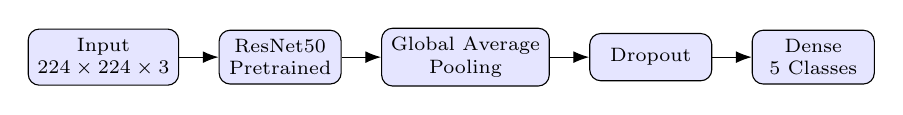
\begin{tikzpicture}[node distance=5mm]

\node[block] (a)
{Input\\$224\times224\times3$};

\node[block,right=of a] (b)
{ResNet50\\Pretrained};

\node[block,right=of b] (c)
{Global Average\\Pooling};

\node[block,right=of c] (d)
{Dropout};

\node[block,right=of d] (e)
{Dense\\5 Classes};

\foreach \x/\y in {a/b,b/c,c/d,d/e}
\draw[arrow] (\x)--(\y);

\end{tikzpicture}

\end{center}

The baseline establishes the reference performance against which the
attention-based models are compared.

% ============================================================
\section*{9. Channel Attention}
% ============================================================

Consider a feature tensor

\[
F\in\mathbb{R}^{H\times W\times C}.
\]

Channel attention determines the relative importance of different feature
channels.

Global average pooling is first used to generate a channel descriptor:

\[
z_c
=
\frac{1}{HW}
\sum_{i=1}^{H}
\sum_{j=1}^{W}
F(i,j,c).
\]

Thus,

\[
z\in\mathbb{R}^{C}.
\]

The channel descriptor is transformed using two learnable transformations:

\[
M_c(F)
=
\sigma
\left(
W_2
\delta
\left(
W_1z
\right)
\right),
\]

where:

\begin{itemize}

\item $\delta(\cdot)$ denotes a nonlinear activation such as ReLU;

\item $\sigma(\cdot)$ denotes the sigmoid activation;

\item $W_1$ reduces the channel representation; and

\item $W_2$ restores the channel dimension.

\end{itemize}

The refined feature tensor is:

\[
F_c
=
F\odot M_c(F).
\]

Channel attention attempts to answer:

\[
\boxed{\text{Which feature channels are important?}}
\]

A reduction ratio of

\[
r=16
\]

may be used as the default setting throughout the laboratory experiment.

The reduction ratio need not be treated as a separate mandatory ablation.

% ============================================================
\section*{10. Spatial Attention}
% ============================================================

Spatial attention determines the spatial regions that should receive greater
importance.

For the input feature tensor

\[
F\in\mathbb{R}^{H\times W\times C},
\]

compute average pooling across channels:

\[
F_{\mathrm{avg}}
=
\operatorname{Mean}_{c}(F),
\]

and maximum pooling across channels:

\[
F_{\mathrm{max}}
=
\operatorname{Max}_{c}(F).
\]

Both tensors have dimensions

\[
H\times W\times1.
\]

Concatenate them:

\[
F_s
=
[
F_{\mathrm{avg}}
\Vert
F_{\mathrm{max}}
].
\]

The spatial attention map is then computed as

\[
M_s(F)
=
\sigma
\left(
\operatorname{Conv}_{7\times7}(F_s)
\right).
\]

Therefore,

\[
M_s(F)
\in
\mathbb{R}^{H\times W\times1}.
\]

The spatially refined feature is

\[
F_s'
=
F\odot M_s(F).
\]

Spatial attention answers:

\[
\boxed{\text{Which spatial locations are important?}}
\]

% ============================================================
\section*{11. Sequential Channel--Spatial Attention}
% ============================================================

Channel and spatial attention can be sequentially applied.

First,

\[
F_c
=
M_c(F)\odot F.
\]

Then,

\[
F_{cs}
=
M_s(F_c)\odot F_c.
\]

The overall structure becomes:

\[
\boxed{
F
\rightarrow
\text{Channel Attention}
\rightarrow
\text{Spatial Attention}
\rightarrow
F_{cs}
}
\]

This arrangement first determines

\[
\text{``what is important''}
\]

and then determines

\[
\text{``where it is important.''}
\]

A simplified diagram is shown below.

\begin{center}

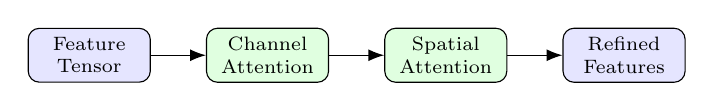
\begin{tikzpicture}[node distance=7mm]

\node[block] (a)
{Feature\\Tensor};

\node[attn,right=of a] (b)
{Channel\\Attention};

\node[attn,right=of b] (c)
{Spatial\\Attention};

\node[block,right=of c] (d)
{Refined\\Features};

\draw[arrow] (a)--(b);
\draw[arrow] (b)--(c);
\draw[arrow] (c)--(d);

\end{tikzpicture}

\end{center}

% ============================================================
\section*{12. Self-Attention}
% ============================================================

Self-attention allows spatial locations to interact directly with other
spatial locations.

For

\[
F\in\mathbb{R}^{H\times W\times C},
\]

flatten the spatial dimensions:

\[
X\in\mathbb{R}^{N\times C},
\]

where

\[
N=HW.
\]

Generate the query, key, and value matrices:

\[
Q=XW_Q,
\]

\[
K=XW_K,
\]

and

\[
V=XW_V.
\]

The attention matrix is

\[
A
=
\operatorname{softmax}
\left(
\frac{QK^T}{\sqrt{d}}
\right),
\]

where $d$ is the dimension of the query/key representation.

The attended output is

\[
Y=AV.
\]

After reshaping the output back to the original spatial structure, a residual
formulation may be used:

\[
F_{\mathrm{SA}}
=
F
+
\gamma
\operatorname{reshape}(Y),
\]

where $\gamma$ is a learnable scaling parameter.

Self-attention attempts to answer:

\[
\boxed{
\text{Which spatial features are related to other spatial features?}
}
\]

Since the attention matrix has dimension approximately

\[
N\times N,
\]

its computational requirements increase rapidly as

\[
N=HW
\]

increases.

Therefore, self-attention should preferably be introduced at

\[
P_3
\]

or

\[
P_4.
\]

% ============================================================
\section*{13. Inserting Attention into ResNet50}
% ============================================================

For any selected stage $P_k$, the network structure can be written as

\[
\text{Previous ResNet Stage}
\rightarrow
\text{Attention}
\rightarrow
\text{Next ResNet Stage}.
\]

For example, attention inserted after conv4\_x gives:

\[
\boxed{
\text{conv4\_x}
\rightarrow
\text{Attention}
\rightarrow
\text{conv5\_x}
}
\]

For channel--spatial attention:

\[
\boxed{
\text{conv4\_x}
\rightarrow
\text{Channel Attention}
\rightarrow
\text{Spatial Attention}
\rightarrow
\text{conv5\_x}
}
\]

The student must record the feature dimensions immediately before and after
the attention block.

Attention should not unintentionally modify the spatial or channel
dimensions unless the selected mechanism explicitly requires such a
transformation.

% ============================================================
\section*{14. Main Experiment 1: Attention-Type Ablation}
% ============================================================

The first experiment studies the effect of different types of attention.

Fix the attention position at

\[
\boxed{
P_3=\text{after conv4\_x}
}
\]

for all models.

Compare the following:

\begin{center}

\begin{tabular}{|l|c|c|c|}
\hline

\textbf{Model}
&
\textbf{Channel}
&
\textbf{Spatial}
&
\textbf{Self-Attention}
\\
\hline

A0: Baseline ResNet50
&
--
&
--
&
--
\\
\hline

A1: Channel Attention
&
$\checkmark$
&
--
&
--
\\
\hline

A2: Spatial Attention
&
--
&
$\checkmark$
&
--
\\
\hline

A3: Channel+Spatial
&
$\checkmark$
&
$\checkmark$
&
--
\\
\hline

A4: Self-Attention
&
--
&
--
&
$\checkmark$
\\
\hline

A5: Combined Attention
&
$\checkmark$
&
$\checkmark$
&
$\checkmark$
\\
\hline

\end{tabular}

\end{center}

This experiment investigates:

\[
\boxed{
\text{How does attention type affect model performance?}
}
\]

Students must keep the following identical:

\begin{itemize}

\item dataset split;

\item preprocessing;

\item augmentation;

\item optimizer;

\item learning rate schedule;

\item epochs;

\item batch size;

\item backbone;

\item classifier;

\item attention position; and

\item evaluation procedure.

\end{itemize}

% ============================================================
\section*{15. Main Experiment 2: Attention-Position Ablation}
% ============================================================

The second experiment investigates the influence of the position of
attention.

Fix the attention type as:

\[
\boxed{
\text{Channel Attention}
\rightarrow
\text{Spatial Attention}
}
\]

and insert exactly the same module at different stages.

\begin{center}

\begin{tabular}{|l|l|c|c|}
\hline

\textbf{Experiment}
&
\textbf{Attention Position}
&
\textbf{Resolution}
&
\textbf{Channels}
\\
\hline

B1
&
After conv2\_x
&
$56\times56$
&
256
\\
\hline

B2
&
After conv3\_x
&
$28\times28$
&
512
\\
\hline

B3
&
After conv4\_x
&
$14\times14$
&
1024
\\
\hline

B4
&
After conv5\_x
&
$7\times7$
&
2048
\\
\hline

\end{tabular}

\end{center}

Students should study whether attention is more beneficial for:

\begin{itemize}

\item high-resolution low-level features;

\item intermediate representations; or

\item low-resolution semantic features.

\end{itemize}

The principal question is:

\[
\boxed{
\text{How does the location of attention influence performance?}
}
\]

% ============================================================
\section*{16. Main Experiment 3: Multiple Attention Positions}
% ============================================================

Attention may also be inserted at more than one ResNet50 stage.

Compare:

\[
\text{Attention only at }P_3,
\]

\[
\text{Attention only at }P_4,
\]

and

\[
\text{Attention at }P_3+P_4.
\]

As an extended experiment, students may evaluate:

\[
P_2+P_3+P_4.
\]

The purpose is to investigate whether applying attention repeatedly provides
sufficient performance improvement to justify the additional:

\begin{itemize}

\item parameters;

\item computation;

\item memory;

\item training time; and

\item inference time.

\end{itemize}

Students should experimentally answer:

\[
\boxed{
\text{Is attention at more locations necessarily more effective?}
}
\]

% ============================================================
\section*{17. Main Experiment 4: Attention Order}
% ============================================================

The sequence in which channel and spatial attention are applied may influence
the resulting features.

Compare:

\[
\boxed{
\text{Channel}
\rightarrow
\text{Spatial}
}
\]

against

\[
\boxed{
\text{Spatial}
\rightarrow
\text{Channel}
}
\]

while maintaining the same insertion position.

For example, at $P_3$:

\[
F
\rightarrow
M_c
\rightarrow
M_s
\]

should be compared with

\[
F
\rightarrow
M_s
\rightarrow
M_c.
\]

Students should determine whether selecting informative feature channels
before selecting spatial regions produces behavior different from selecting
spatial regions first.

% ============================================================
\section*{18. Main Experiment 5: Spatial Attention Kernel Size}
% ============================================================

The receptive field used to generate the spatial attention map may influence
the result.

Evaluate:

\[
k\in\{3,5,7\}.
\]

Use the same attention position and training protocol.

\begin{center}

\begin{tabular}{|c|c|c|c|}
\hline

\textbf{Spatial Kernel}
&
\textbf{Accuracy}
&
\textbf{Macro F1}
&
\textbf{Inference Time}
\\
\hline

$3\times3$
& 0.920145 
& 0.918573 
& 9.194100 ms/image
\\
\hline

$5\times5$
& 0.903811
& 0.902608
& 9.376349 ms/image
\\
\hline

$7\times7$
& 0.918330
& 0.917174
& 10.171732 ms/image
\\
\hline

\end{tabular}

\end{center}

Students should discuss whether a larger spatial kernel provides a useful
increase in contextual information.

% ============================================================
\section*{19. Additional Task: Comparison of Different Attention Mechanisms}
% ============================================================

As an additional exploration task, students should compare the attention
mechanisms implemented in the laboratory with established attention
approaches.

Students should select at least

\[
\boxed{\text{two additional attention mechanisms}}
\]

from the following:

\begin{itemize}

\item Squeeze-and-Excitation (SE) Attention;

\item Efficient Channel Attention (ECA);

\item Convolutional Block Attention Module (CBAM);

\item Coordinate Attention; and

\item lightweight Self-Attention.

\end{itemize}

The pretrained backbone must remain:

\[
\boxed{\text{ResNet50}}
\]

for all comparisons.

To ensure a fair comparison, additional attention mechanisms should
preferably be inserted at the same position:

\[
\boxed{
P_3=\text{after conv4\_x}
}
\]

unless the student provides a technical justification for using another
location.

% ============================================================
\subsection*{19.1 Suggested Comparison}
% ============================================================

\begin{center}

\resizebox{\textwidth}{!}{
\begin{tabular}{|l|c|c|c|c|c|c|}
\hline

\textbf{Attention}
&
\textbf{Accuracy}
&
\textbf{Precision}
&
\textbf{Recall}
&
\textbf{Macro F1}
&
\textbf{Parameters}
&
\textbf{Inference Time}
\\
\hline

No Attention
& 0.9110
& 0.9095
& 0.9119
& 0.9097
& 23597957
& 8.634829646875156 ms/image
\\
\hline

Channel Attention
& 0.9274
& 0.9258
& 0.9292
& 0.9264
& 23730117
& 8.7094 ms/image
\\
\hline

Spatial Attention
& 0.9382
& 0.9374
& 0.9380
& 0.9377
& 23598056
& 8.1750 ms/image
\\
\hline

CBAM
& 0.9255
& 0.9246
& 0.9257
& 0.9241
& 23730216
& 9.1991 ms/image
\\
\hline

Self-Attention
& 0.9292
& 0.9298
& 0.9282
& 0.9289
& 24123654
& 8.7315 ms/image
\\

\hline

\end{tabular}}
\end{center}

% ============================================================
\subsection*{19.2 Questions for Attention-Mechanism Comparison}
% ============================================================

Students should investigate:

\begin{enumerate}

\item \textbf{How does classification accuracy vary across attention mechanisms?}

\textbf{Answer:} Classification accuracy is usually improved if attention mechanisms are used against the baseline network. Combination of both channel and spatial attention modules usually leads to greater accuracy, because both types of features are refined. However, some attention mechanisms that are poorly tuned or too complex may provide little improvement or even degrade accuracy due to overfitting.

\vspace{5mm}

\item \textbf{How does macro F1-score vary across attention mechanisms?}

\textbf{Answer:}  Macro F1-score becomes higher as attention helps the model to differentiate visually similar flower classes. Since macro F1-score considers equally all classes, it reflects improvements made in both easy and hard categories. Combined attention mechanisms usually provide the highest and balanced macro F1-scores.

\vspace{5mm}

\item \textbf{How many parameters are introduced by each attention module?}

\textbf{Answer:} Introduced parameters depend on the design of the attention module. Ultra-lightweight mechanisms like ECA require zero additional parameters. Squeeze-and-Excitation requires a small number of parameters as the fully-connected layers. Self-attention modules introduce much parameters because of linear projection matrices.

\vspace{5mm}

\item \textbf{How does each attention mechanism influence inference time?}

\textbf{Answer:} Light channel attention mechanisms contribute insignificantly to computation, which leads to almost the same inference times as the baseline. Spatial attention increases latency slightly due to the two-dimensional convolution operations over feature maps. Self-attention brings additional latency because of the calculations of pairwise interaction across all spatial locations.

\vspace{5mm}

\item \textbf{Does attention improve the convergence behavior?}

\textbf{Answer:} Yes, attention mechanisms tend to enhance the convergence behavior due to clearer feature
signals and gradients. Models with attention achieve significantly lower training losses in a lesser number of epochs than the baseline model. The result is smoother learning curves and more stable validation accuracies.

\vspace{5mm}

\item \textbf{Does attention produce more focused feature localization?}

\textbf{Answer:} Yes, attention mechanisms actively adjust feature maps to focus high activations on the target object. Heatmaps for attention mechanisms tend to demonstrate more concentrated clusters around discriminating flower petals and centers. Feature maps for irrelevant background regions like grass or leaves get significantly fewer activations than other mechanisms.

\vspace{5mm}

\item \textbf{Does an increase in attention complexity always improve classification performance?}

\textbf{Answer:} No, an increase in the complexity of an attention module does not lead to an increase in classification accuracy. Very complex models having numerous parameters might lead to overfitting, thus making training and inference slow. Often, simpler and more efficient mechanisms perform as good or even better compared to complicated ones.

\vspace{5mm}

\item \textbf{Does a lightweight attention mechanism provide comparable performance with a computationally heavier mechanism?}

\textbf{Answer:}  Yes, often the performance of a lightweight mechanism is on par or exceeds the performance of a computationally more intensive one. The reason for this lies in the fact that the lightweight mechanism does not employ extreme dimensionality reduction or very complex architecture, which allows preserving visual information well enough.
 
\vspace{5mm}

\end{enumerate}

The objective is to understand:

\[
\boxed{
\text{Performance}
+
\text{Complexity}
+
\text{Attention Behaviour}
}
\]

rather than considering only classification accuracy.

% ============================================================
\section*{20. Transfer-Learning Strategy}
% ============================================================

Use ImageNet pretrained weights.

A recommended training strategy is:

\begin{enumerate}

\item Load ResNet50 with ImageNet pretrained weights.

\item Remove the original ImageNet classification layer.

\item Insert the selected attention module.

\item Add Global Average Pooling.

\item Add Dropout.

\item Add a Dense classification layer containing five output neurons.

\item Initially freeze the pretrained ResNet50 layers.

\item Train the newly introduced attention and classification layers.

\item Unfreeze the final ResNet50 stage or selected final stages.

\item Fine-tune the network using a smaller learning rate.

\end{enumerate}

A suitable initial learning rate for the newly introduced layers is

\[
10^{-3}.
\]

During fine-tuning, a smaller learning rate such as

\[
10^{-5}
\quad\text{to}\quad
10^{-4}
\]

may be used.

The exact values selected by the student should remain identical for all
controlled comparisons.

% ============================================================
\section*{21. Loss Function}
% ============================================================

For the five-class classification problem, use categorical cross-entropy.

For $N$ samples:

\[
\mathcal{L}_{CE}
=
-
\frac{1}{N}
\sum_{i=1}^{N}
\sum_{c=1}^{5}
y_{i,c}
\log
\widehat{y}_{i,c},
\]

where:

\[
y_{i,c}
\]

is the ground-truth label and

\[
\widehat{y}_{i,c}
\]

is the predicted probability.

The same loss formulation must be used for every attention comparison.

% ============================================================
\section*{22. Evaluation Metrics}
% ============================================================

Students must report the following quantitative metrics:

\begin{itemize}

\item classification accuracy;

\item macro precision;

\item macro recall;

\item macro F1-score;

\item number of trainable parameters;

\item total number of parameters; and

\item average inference time per image.

\end{itemize}

For class $c$,

\[
\mathrm{Precision}_c
=
\frac{TP_c}
{TP_c+FP_c},
\]

\[
\mathrm{Recall}_c
=
\frac{TP_c}
{TP_c+FN_c},
\]

and

\[
F1_c
=
2
\frac{
\mathrm{Precision}_c
\mathrm{Recall}_c
}{
\mathrm{Precision}_c+
\mathrm{Recall}_c
}.
\]

Macro F1 is:

\[
\mathrm{Macro\ F1}
=
\frac{1}{C}
\sum_{c=1}^{C}
F1_c,
\]

where

\[
C=5.
\]

% ============================================================
\section*{23. Required Main Result Table}
% ============================================================

Students should summarize the major experiments using the following table.

\begin{center}

\resizebox{\textwidth}{!}{
\begin{tabular}{|l|l|c|c|c|c|c|c|}
\hline

\textbf{Model}
&
\textbf{Position}
&
\textbf{Accuracy}
&
\textbf{Precision}
&
\textbf{Recall}
&
\textbf{F1}
&
\textbf{Parameters}
&
\textbf{Inference Time}
\\
\hline

Baseline
&
--
& 0.9110
& 0.9095
& 0.9119
& 0.9097
& 23597957
& 8.6348 ms/image
\\
\hline

Channel Attention
&
$P_3$
& 0.9274
& 0.9258
& 0.9292
& 0.9264
& 23730117
& 8.7094 ms/image
\\
\hline

Spatial Attention
&
$P_3$
& 0.9382
& 0.9374
& 0.9380
& 0.9377
& 23598056
& 8.1750 ms/image
\\
\hline

Channel+Spatial
&
$P_2$
& 0.9128
& 0.9124
& 0.9144
& 0.9129
& 23631368
& 9.1226 ms/image
\\
\hline

Channel+Spatial
&
$P_3$
& 0.9292
& 0.9272
& 0.9307
& 0.9280
& 23730216
& 9.5715 ms/image
\\
\hline

Channel+Spatial
&
$P_4$
& 0.9255
& 0.9246
& 0.9241
& 0.9238
& 24124520
& 9.6524 ms/image
\\
\hline

Self-Attention
&
$P_3$
& 0.9292
& 0.9298
& 0.9282
& 0.9289
& 24123654
& 8.7315 ms/image
\\
\hline

CBAM
&
$P_3$
& 0.9255
& 0.9246
& 0.9257
& 0.9241
& 23730216
& 9.1991 ms/image
\\
\hline

Squeeze and Excitation Attention
&
$P_3$
& 0.9401
& 0.9379
& 0.9421
& 0.9393
& 23730117
& 8.7895 ms/image
\\
\hline

\end{tabular}}
\end{center}

% ============================================================
\section*{24. Graphical Performance Analysis}
% ============================================================

Students should not present only numerical tables.

Appropriate graphs must be generated to analyze model behavior.

At least three of the following graphical comparisons should be included in
the laboratory report.

% ============================================================
\subsection*{24.1 Training and Validation Accuracy}
% ============================================================

Plot

\[
\text{Epoch}
\quad\text{versus}\quad
\text{Accuracy}
\]

for:

\begin{itemize}

\item baseline ResNet50; and

\item selected attention models.

\end{itemize}

Both training and validation accuracy should be shown.

Students should comment on whether attention:

\begin{itemize}

\item accelerates convergence;

\item produces smoother learning;

\item reduces the train--validation gap;

\item leads to overfitting; or

\item causes unstable training.

\end{itemize}

% ============================================================
\subsection*{24.2 Training and Validation Loss}
% ============================================================

Plot

\[
\text{Epoch}
\quad\text{versus}\quad
\mathcal{L}_{CE}.
\]

The graph should include training and validation loss.

Students should compare the convergence behavior of the baseline and
attention models.

% ============================================================
\subsection*{24.3 Attention Mechanism versus Accuracy}
% ============================================================

Generate a bar graph:

\[
x=
\text{Attention Mechanism}
\]

and

\[
y=
\text{Classification Accuracy}.
\]

Possible entries are:

\begin{center}

Baseline,
Channel,
Spatial,
Channel+Spatial,
Self-Attention,
SE,
ECA,
CBAM.

\end{center}

% ============================================================
\subsection*{24.4 Attention Mechanism versus Macro F1}
% ============================================================

Similarly, plot:

\[
x=
\text{Attention Mechanism}
\]

and

\[
y=
\text{Macro F1-score}.
\]

This comparison is useful when the class-wise performance is not uniform.

% ============================================================
\subsection*{24.5 Accuracy versus Model Parameters}
% ============================================================

Create a scatter plot using:

\[
x=
\text{Total Model Parameters}
\]

and

\[
y=
\text{Test Accuracy}.
\]

Each point should represent one attention mechanism.

This allows the student to study the

\[
\boxed{
\text{Accuracy--Complexity Trade-off}
}
\]

instead of evaluating accuracy independently.

% ============================================================
\subsection*{24.6 Macro F1 versus Inference Time}
% ============================================================

Plot:

\[
x=
\text{Inference Time per Image}
\]

and

\[
y=
\text{Macro F1-score}.
\]

Students should analyze whether additional computational cost produces a
meaningful increase in classification performance.

% ============================================================
\section*{25. Confusion Matrix Analysis}
% ============================================================

Generate a confusion matrix for:

\begin{enumerate}

\item baseline ResNet50; and

\item the selected attention-based ResNet50.

\end{enumerate}

The confusion matrix should contain all five flower classes.

Students should analyze:

\begin{itemize}

\item which classes are most accurately classified;

\item which classes are frequently confused;

\item which class benefits most from attention;

\item whether attention reduces a particular type of confusion; and

\item whether the improved overall accuracy is distributed across classes.

\end{itemize}

% ============================================================
\section*{26. Qualitative Analysis of Attention}
% ============================================================

Quantitative classification performance does not directly explain where the
network obtains evidence for its prediction.

Students must therefore perform qualitative analysis.

The visual analysis should include:

\begin{itemize}

\item internal attention maps;

\item attention overlays;

\item intermediate feature maps; and

\item Grad-CAM explanations.

\end{itemize}

Students should preferably use the same input image when comparing different
models.

% ============================================================
\section*{27. Grad-CAM Visualization}
% ============================================================

Gradient-weighted Class Activation Mapping (Grad-CAM) provides a
class-specific visualization of the regions contributing to a prediction.

Let

\[
A^k
\]

represent feature map $k$ from a selected convolutional layer.

For class score $y^c$, the importance coefficient is:

\[
\alpha_k^c
=
\frac{1}{HW}
\sum_i
\sum_j
\frac{\partial y^c}
{\partial A_{ij}^k}.
\]

The Grad-CAM map is:

\[
L_{\mathrm{Grad-CAM}}^c
=
\operatorname{ReLU}
\left(
\sum_k
\alpha_k^c A^k
\right).
\]

The map should be resized to the original image resolution and overlaid on
the input.

Students should compare:

\[
\boxed{
\text{Input}
\;|\;
\text{Baseline Grad-CAM}
\;|\;
\text{Attention Model Grad-CAM}
}
\]

for the same image.

% ============================================================
\subsection*{27.1 Grad-CAM Interpretation}
% ============================================================

Students should qualitatively determine whether the attention model:

\begin{itemize}

\item focuses more strongly on the flower;

\item suppresses irrelevant background regions;

\item concentrates on petals;

\item concentrates on the central flower structure;

\item attends to discriminative edges;

\item distributes activation across the entire flower;

\item incorrectly focuses on leaves;

\item incorrectly focuses on background objects; or

\item changes its focus for an incorrect prediction.

\end{itemize}

Students should avoid unsupported statements such as:

\begin{quote}
``The Grad-CAM of Model A is better.''
\end{quote}

Instead, the observation should describe visible evidence.

For example:

\begin{quote}
The baseline network activates both the flower and surrounding leaves,
whereas the attention-based model produces stronger activation over the petal
region and weaker activation over the background.
\end{quote}

% ============================================================
\section*{28. Internal Attention Maps}
% ============================================================

An important objective of this experiment is to distinguish between:

\[
\boxed{\text{Internal Attention}}
\]

and

\[
\boxed{\text{Post-hoc Explanation}}
\]

because they are not the same.

An attention module directly computes weights during the forward pass.

Grad-CAM, in contrast, is generated after prediction using gradients.

% ============================================================
\subsection*{28.1 Channel-Attention Visualization}
% ============================================================

For channel attention:

\[
M_c(F)
=
[m_1,m_2,\ldots,m_C].
\]

Students should visualize the learned channel importance values using a bar
graph.

Instead of displaying every channel when $C$ is large, the student may show
the top-$K$ channels.

Recommended values are:

\[
K=10
\]

or

\[
K=20.
\]

Students should comment on whether:

\begin{itemize}

\item a small number of channels receive strong weights;

\item many channels contribute similarly; or

\item channel weighting changes substantially for different input images.

\end{itemize}

% ============================================================
\subsection*{28.2 Spatial-Attention Visualization}
% ============================================================

For spatial attention:

\[
M_s(F)
\in
\mathbb{R}^{H\times W}.
\]

Resize the attention map to:

\[
224\times224
\]

and overlay it on the input image.

Display:

\[
\boxed{
\text{Input}
\;|\;
\text{Spatial Attention Map}
\;|\;
\text{Attention Overlay}
}
\]

Students should identify the image regions receiving high attention values.

% ============================================================
\subsection*{28.3 Self-Attention Visualization}
% ============================================================

For self-attention, students may visualize one of the following:

\begin{itemize}

\item attention associated with a selected query location;

\item mean attention across query positions;

\item maximum attention across query positions; or

\item an aggregated spatial self-attention response.

\end{itemize}

The visualization should be reshaped into a spatial form and, when
appropriate, resized to the image resolution.

Students should analyze how distant regions interact within the feature map.

% ============================================================
\section*{29. Attention Position Visualization}
% ============================================================

Use the same test image to visualize spatial attention at different ResNet50
stages.

Generate:

\[
M_s^{P_2},
\qquad
M_s^{P_3},
\qquad
M_s^{P_4}.
\]

Display the maps as:

\[
\boxed{
\text{Input}
\;|\;
M_s^{P_2}
\;|\;
M_s^{P_3}
\;|\;
M_s^{P_4}
}
\]

The objective is to visually study how attention changes as feature
representations become deeper.

Possible observations may include:

\begin{itemize}

\item $P_2$ responding strongly to edges, colors, textures, and fine
structures;

\item $P_3$ responding to flower parts and intermediate object structures;

\item $P_4$ responding to larger semantic flower regions.

\end{itemize}

These observations must be based on the student's experimental
visualizations.



% ============================================================
\section*{30. Plots and Inference}
% ============================================================

% ------------------------------------------------------------
\subsection*{30.1 Dataset Sample Images}
% ------------------------------------------------------------

\begin{figure}[H]
\centering

\includegraphics[width=\textwidth]{Images/use/sample_images.png}
\caption{Sample images from the TensorFlow Flower dataset}
\label{fig:sample_images}
\end{figure}

\textbf{Inference:} This dataset shows notable heterogeneity in visual appearance across the five flower classes with respect to scale differences, lighting conditions, camera view angles, and natural background clutter such as leaves, soil, and garden elements. Flower species such as daisy and dandelion have similar petal structure radially symmetric; roses and tulips, on the other hand, have similar chromatic properties and densely packed petals. This difficult class variation calls for the use of selective attention to extract the flower objects from background clutter.

\vspace{3mm}

% ------------------------------------------------------------
\subsection*{30.2 Baseline ResNet50: Accuracy, Loss, and Confusion Matrix}
% ------------------------------------------------------------

\begin{figure}[H]
\centering
\begin{subfigure}[b]{0.485\textwidth}
    \centering
    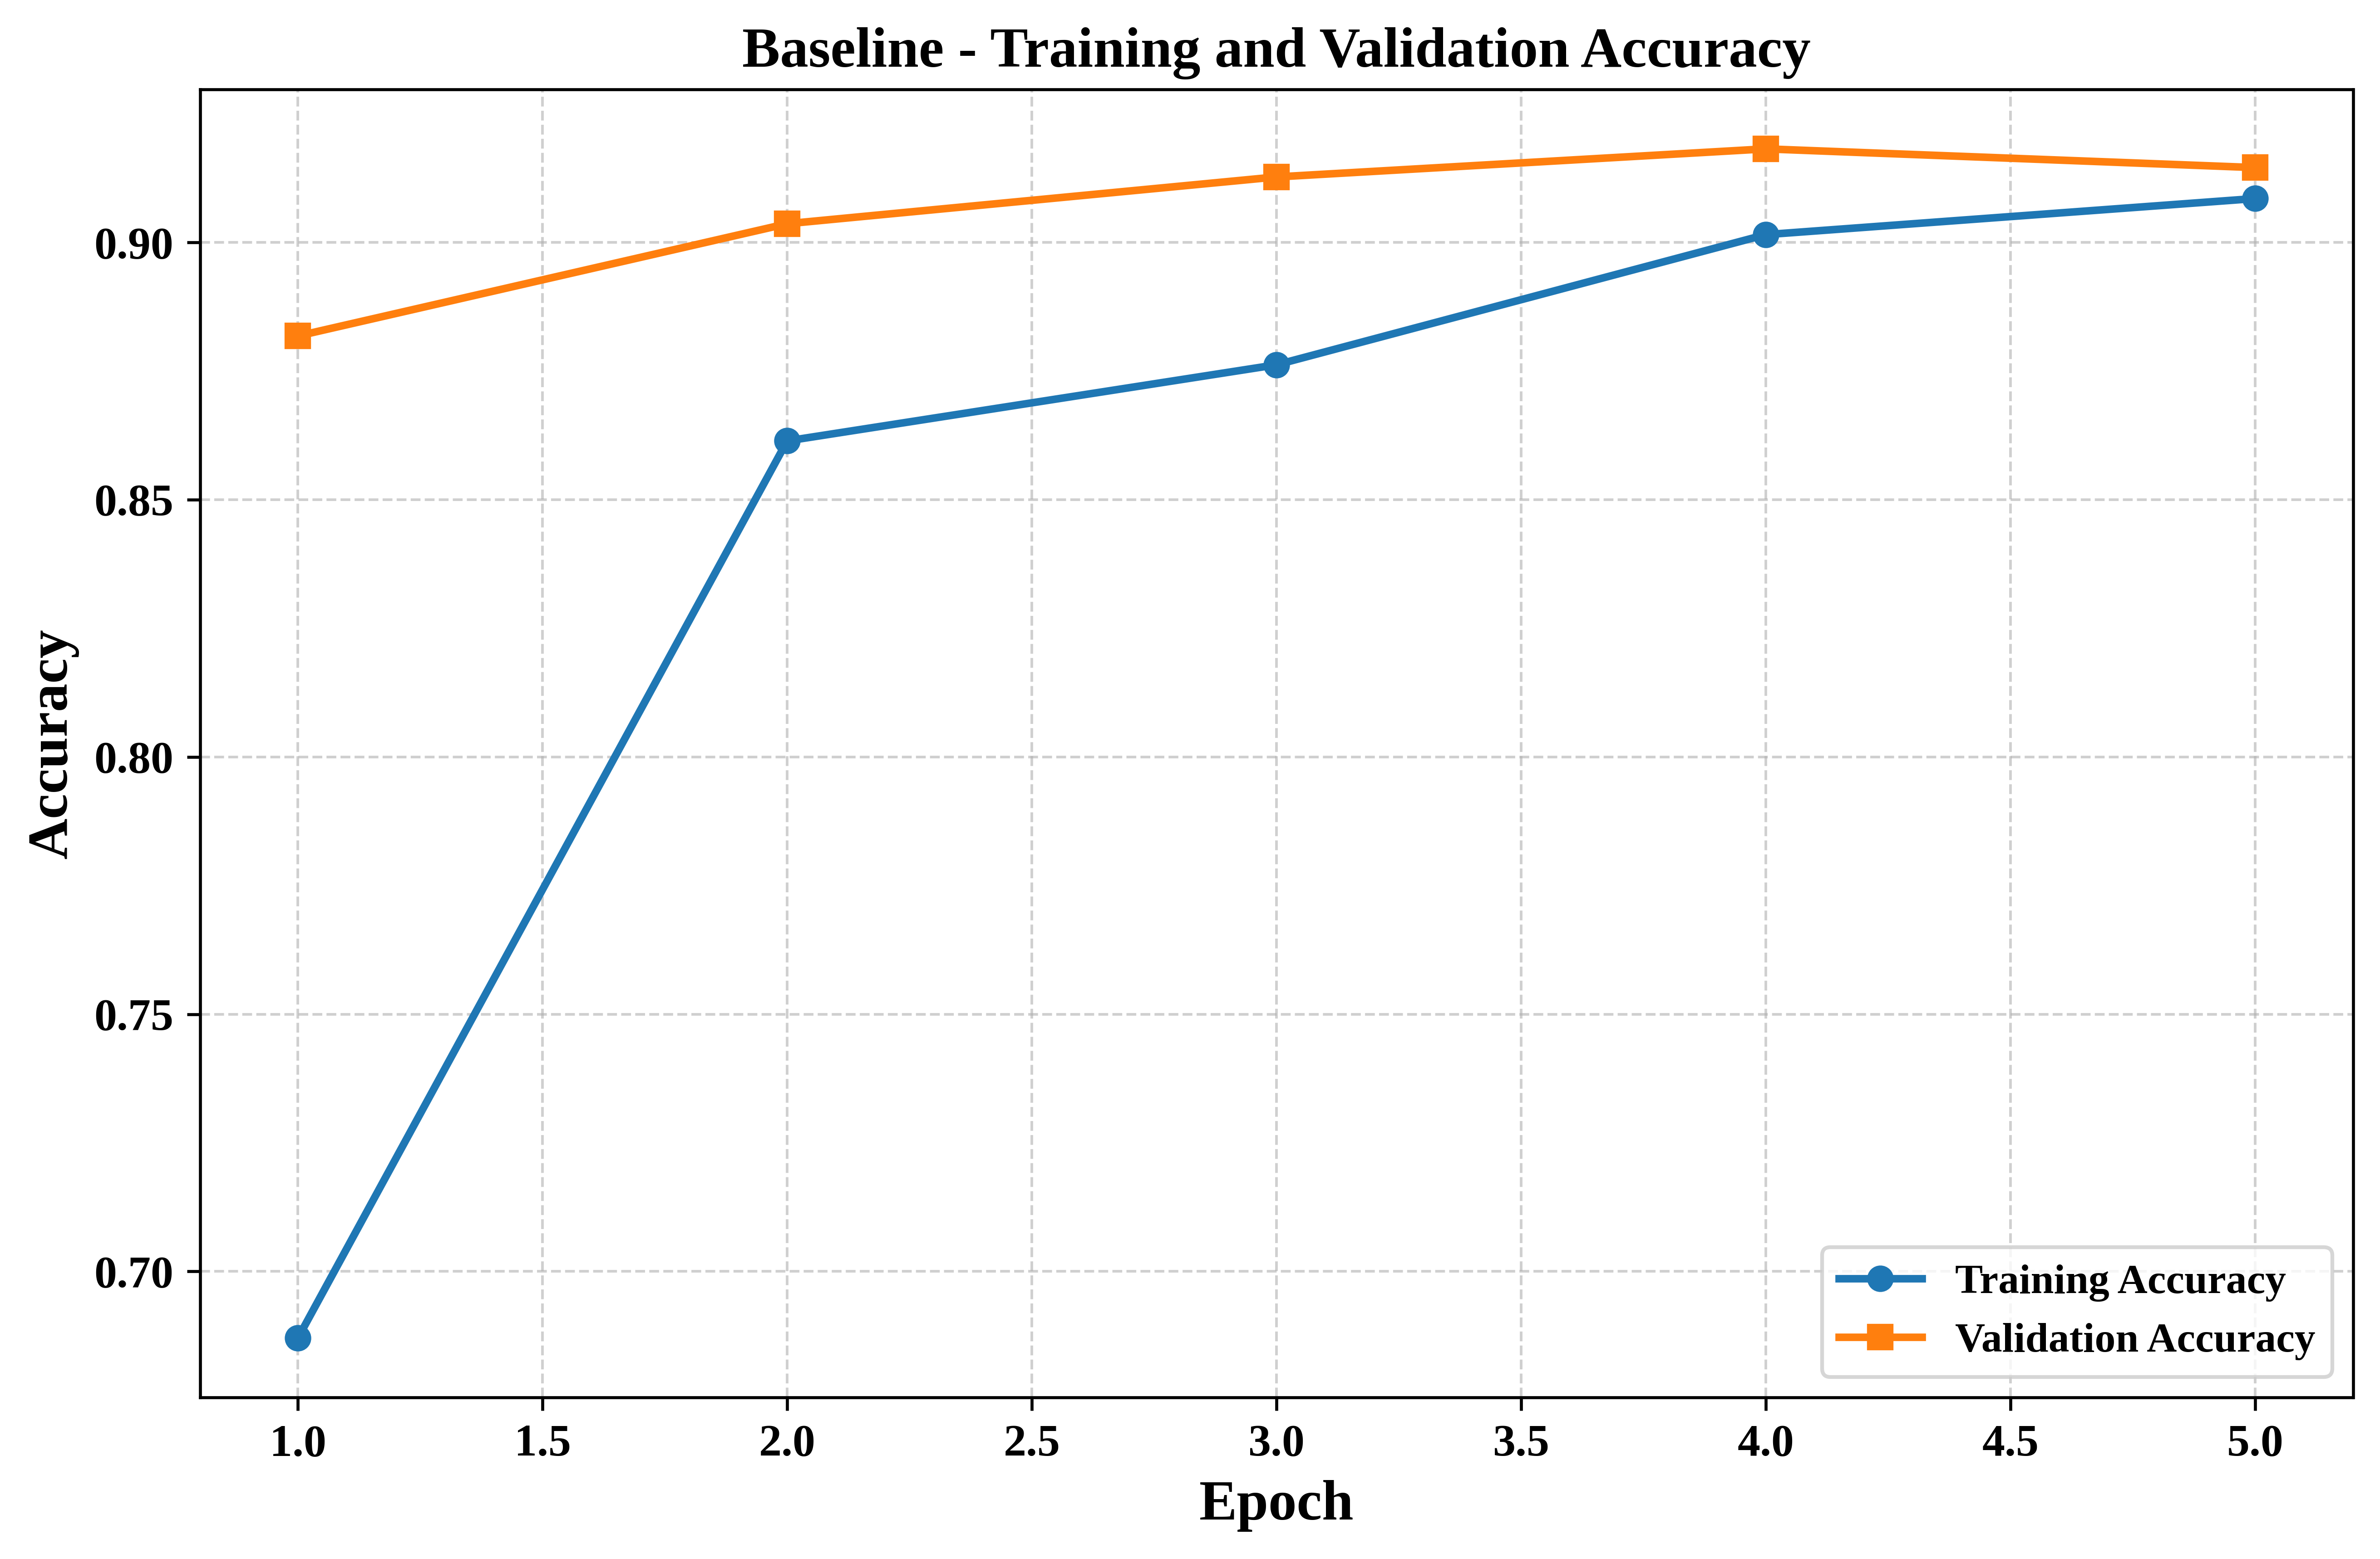
\includegraphics[width=\linewidth]{Images/use/baseline_accuracy.png}
    \caption{Training and Validation Accuracy}
\end{subfigure}
\hfill
\begin{subfigure}[b]{0.485\textwidth}
    \centering
    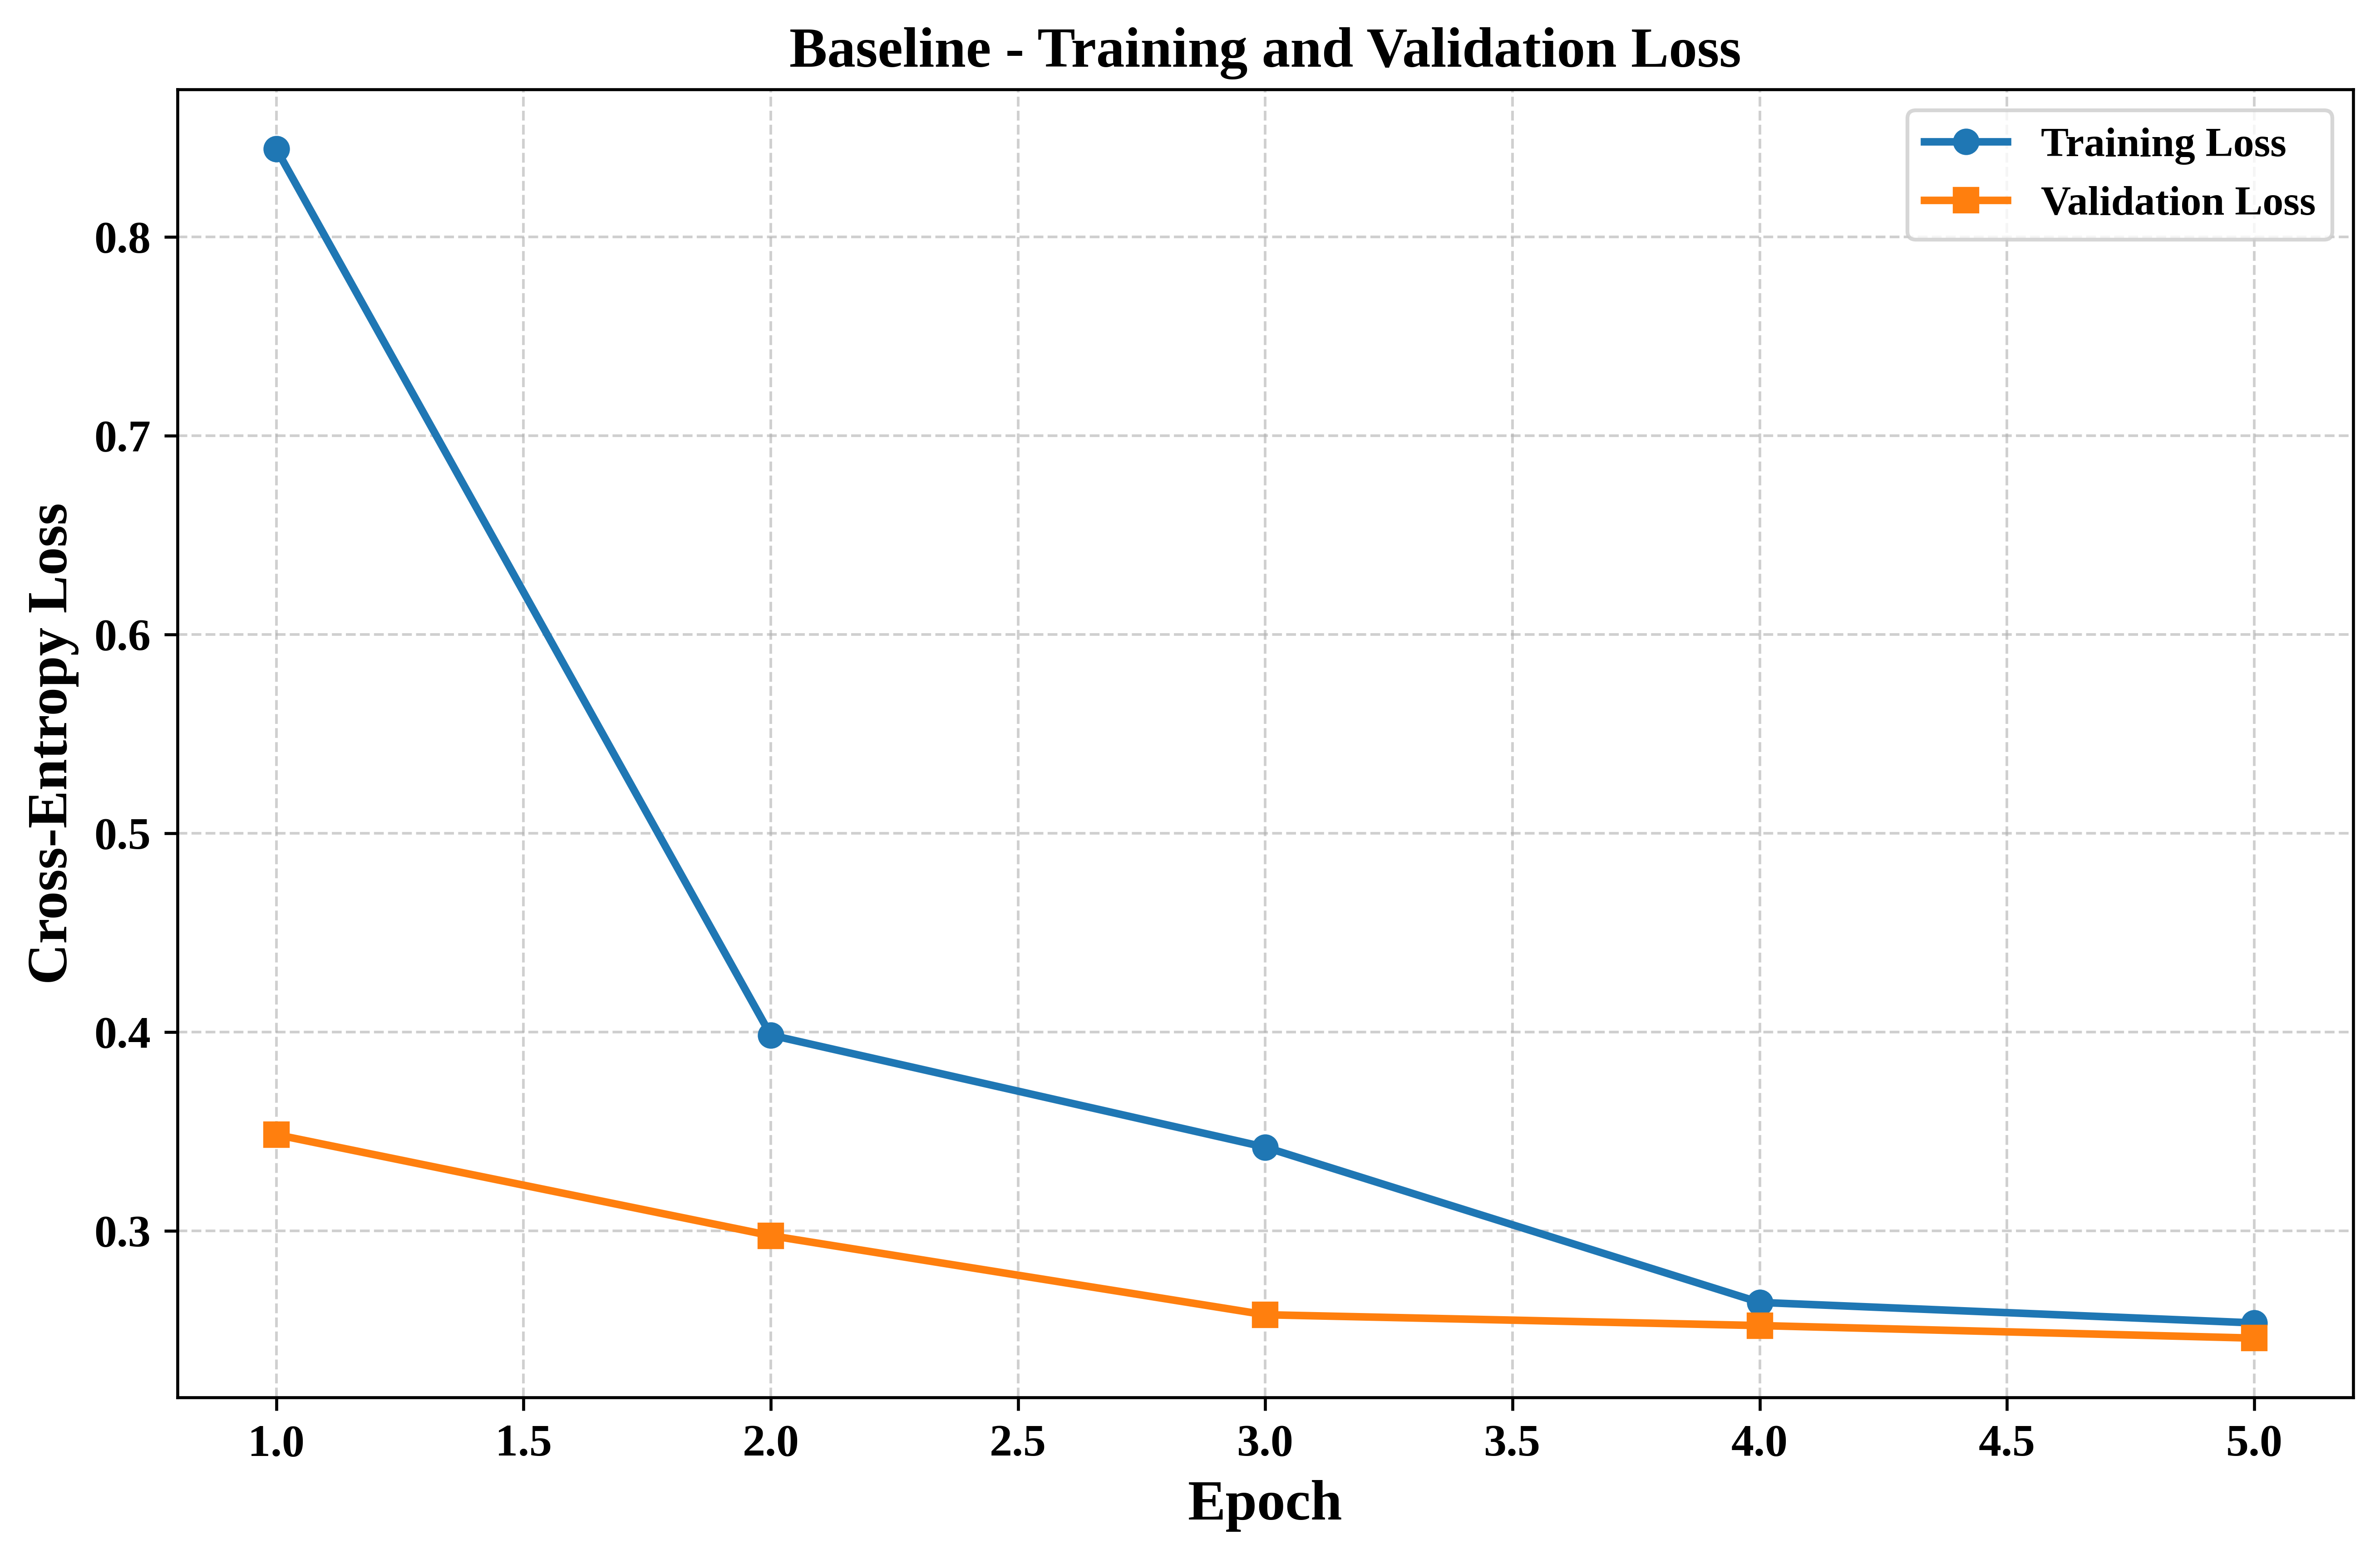
\includegraphics[width=\linewidth]{Images/use/baseline_loss.png}
    \caption{Training and Validation Loss}
\end{subfigure}

\vspace{2mm}
\begin{subfigure}[b]{0.44\textwidth}
    \centering
    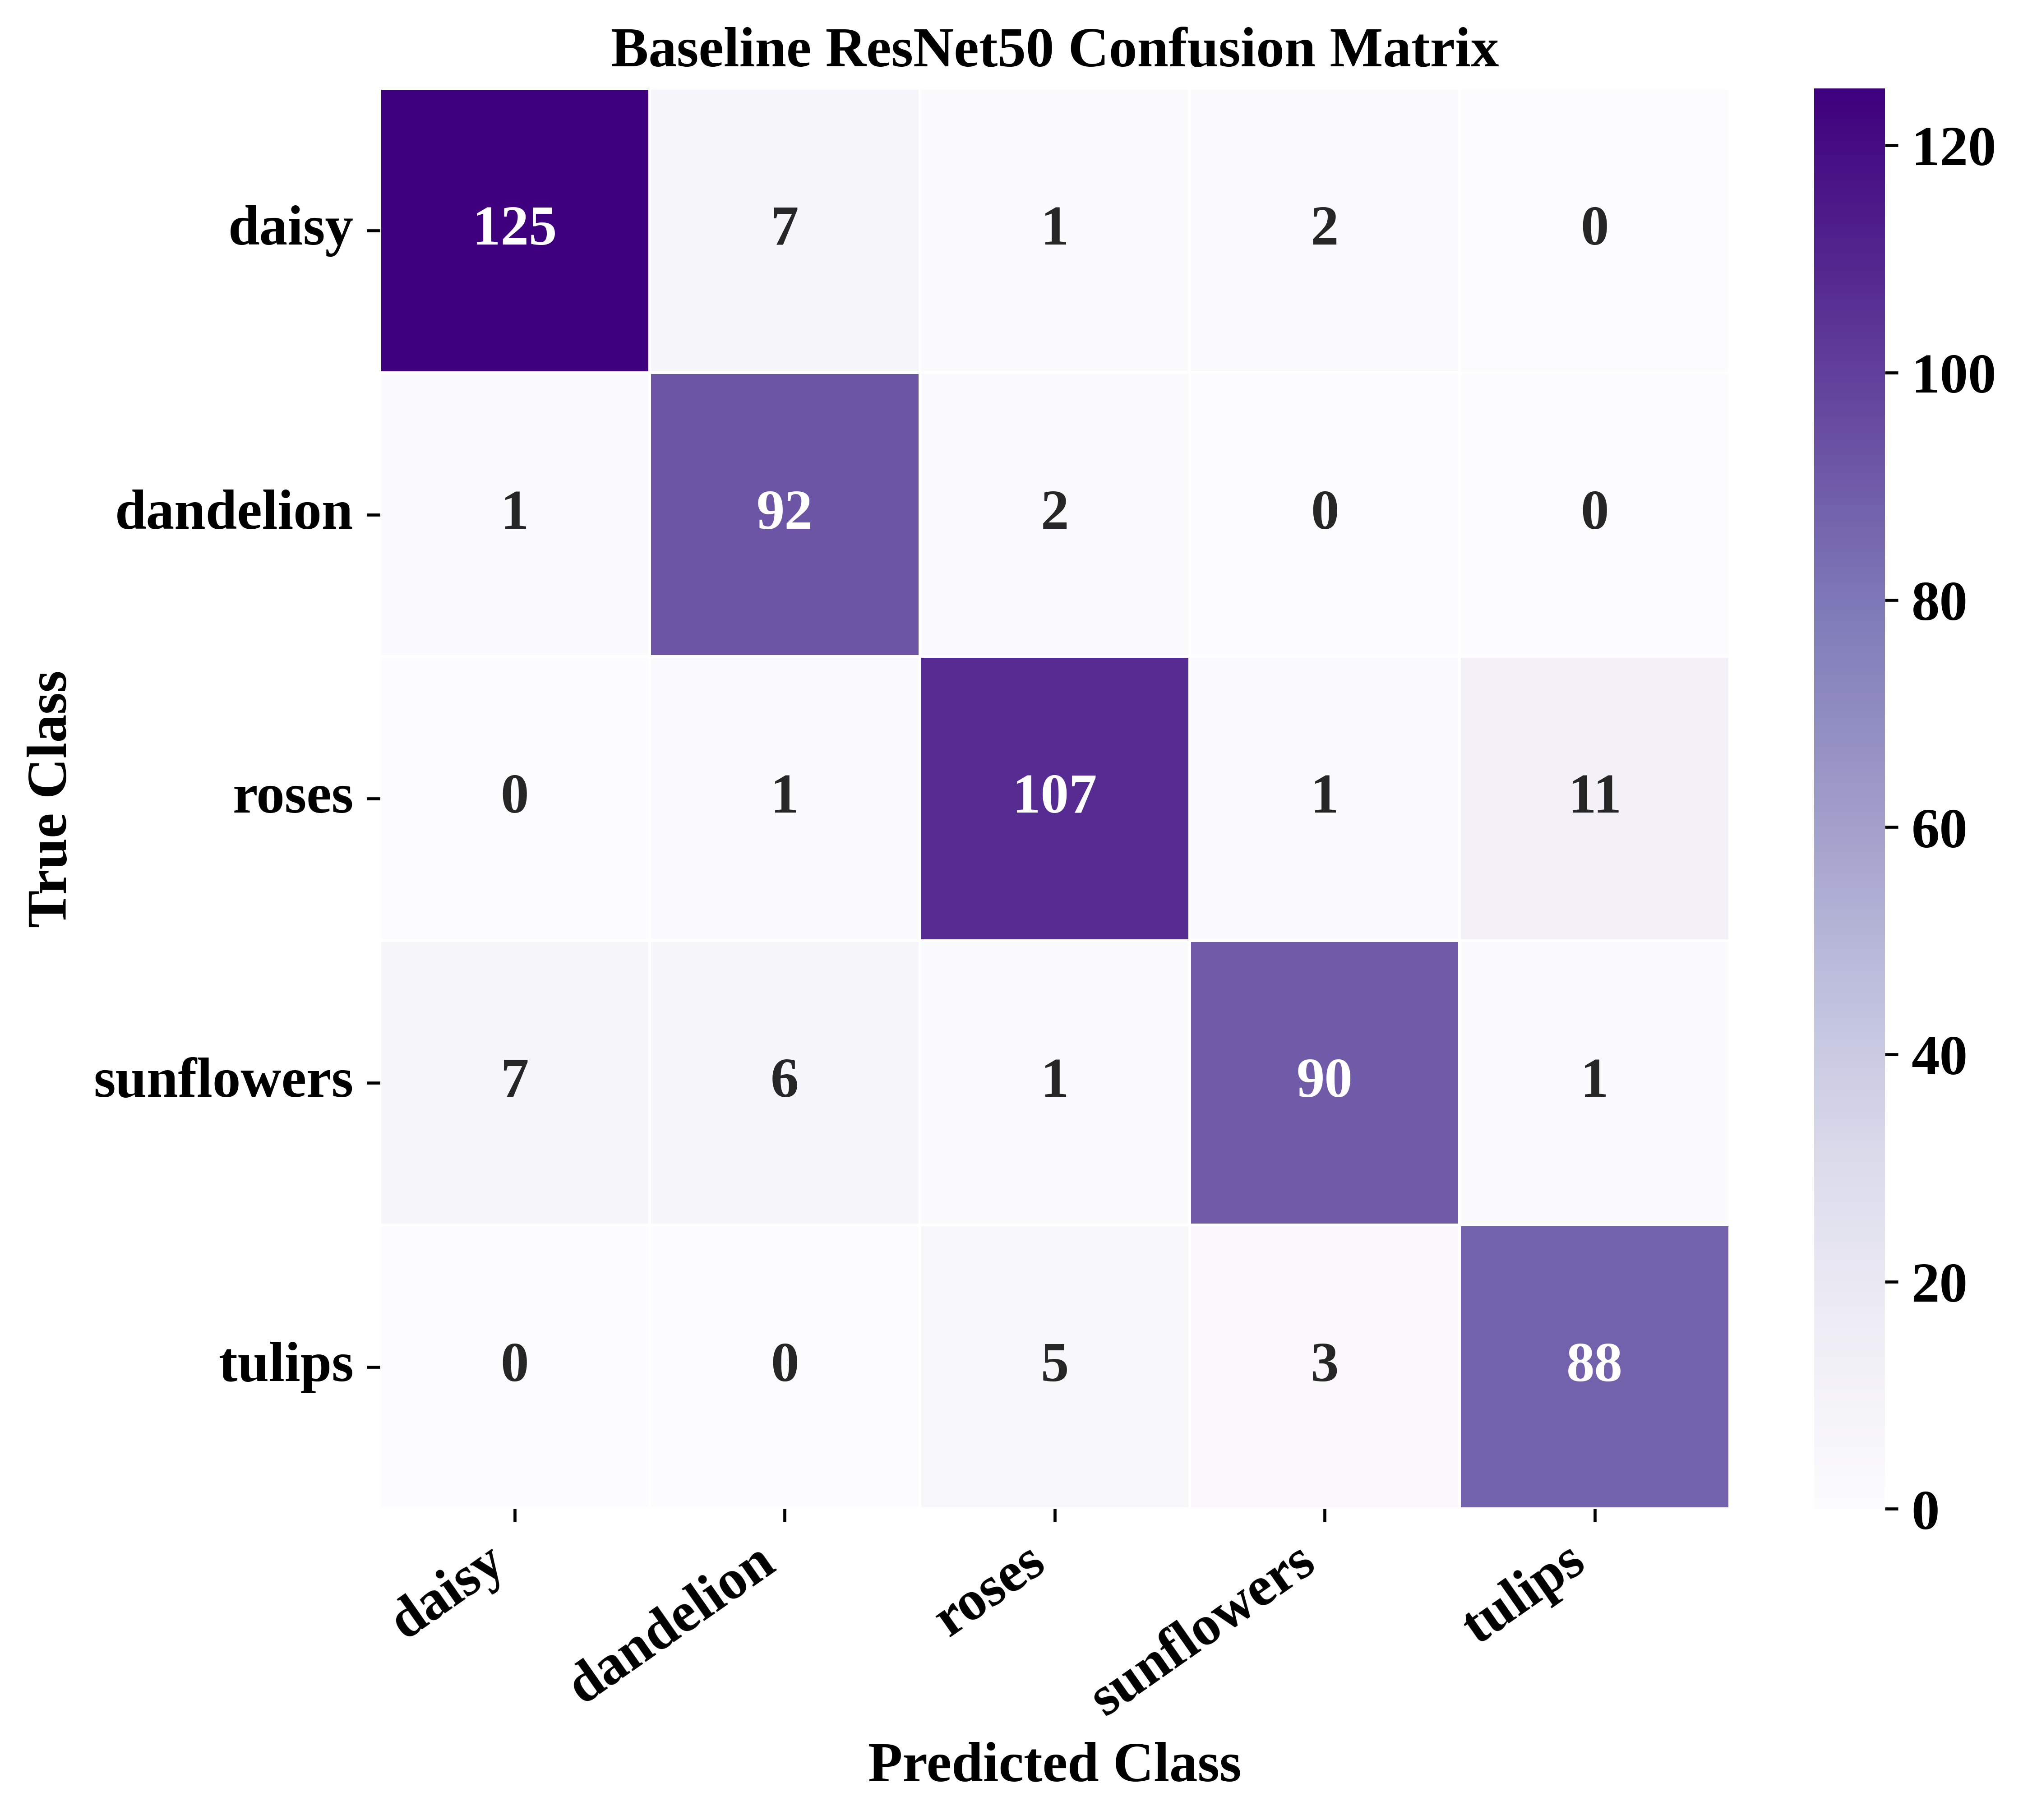
\includegraphics[width=\linewidth]{Images/use/baseline_confusion_matrix.png}
    \caption{Test Confusion Matrix}
\end{subfigure}
\caption{Baseline Pretrained ResNet50: Training and validation accuracy curves, cross-entropy loss trajectories across fine-tuning epochs, and resulting test confusion matrix.}
\label{fig:baseline_group}
\end{figure}

\textbf{Inference:} The ResNet50 baseline shows quick and stable convergence with final validation accuracy reaching about 91.5\% and training accuracy showing low overfitting with almost identical values. Cross entropy loss decreases gradually from 0.85 to 0.25, demonstrating good gradient updates from ImageNet initialization. Confusion matrix in test set shows good accuracy of daisy (125 correct) and dandelion (92 correct). Misclassification is mostly found between roses and tulips (11 roses are classified as tulips) owing to similar coloration and morphology.

\vspace{3mm}

% ------------------------------------------------------------
\subsection*{30.3 Channel Attention at $P_3$ (conv4\_x): Accuracy, Loss, and Confusion Matrix}
% ------------------------------------------------------------

\begin{figure}[H]
\centering
\begin{subfigure}[b]{0.485\textwidth}
    \centering
    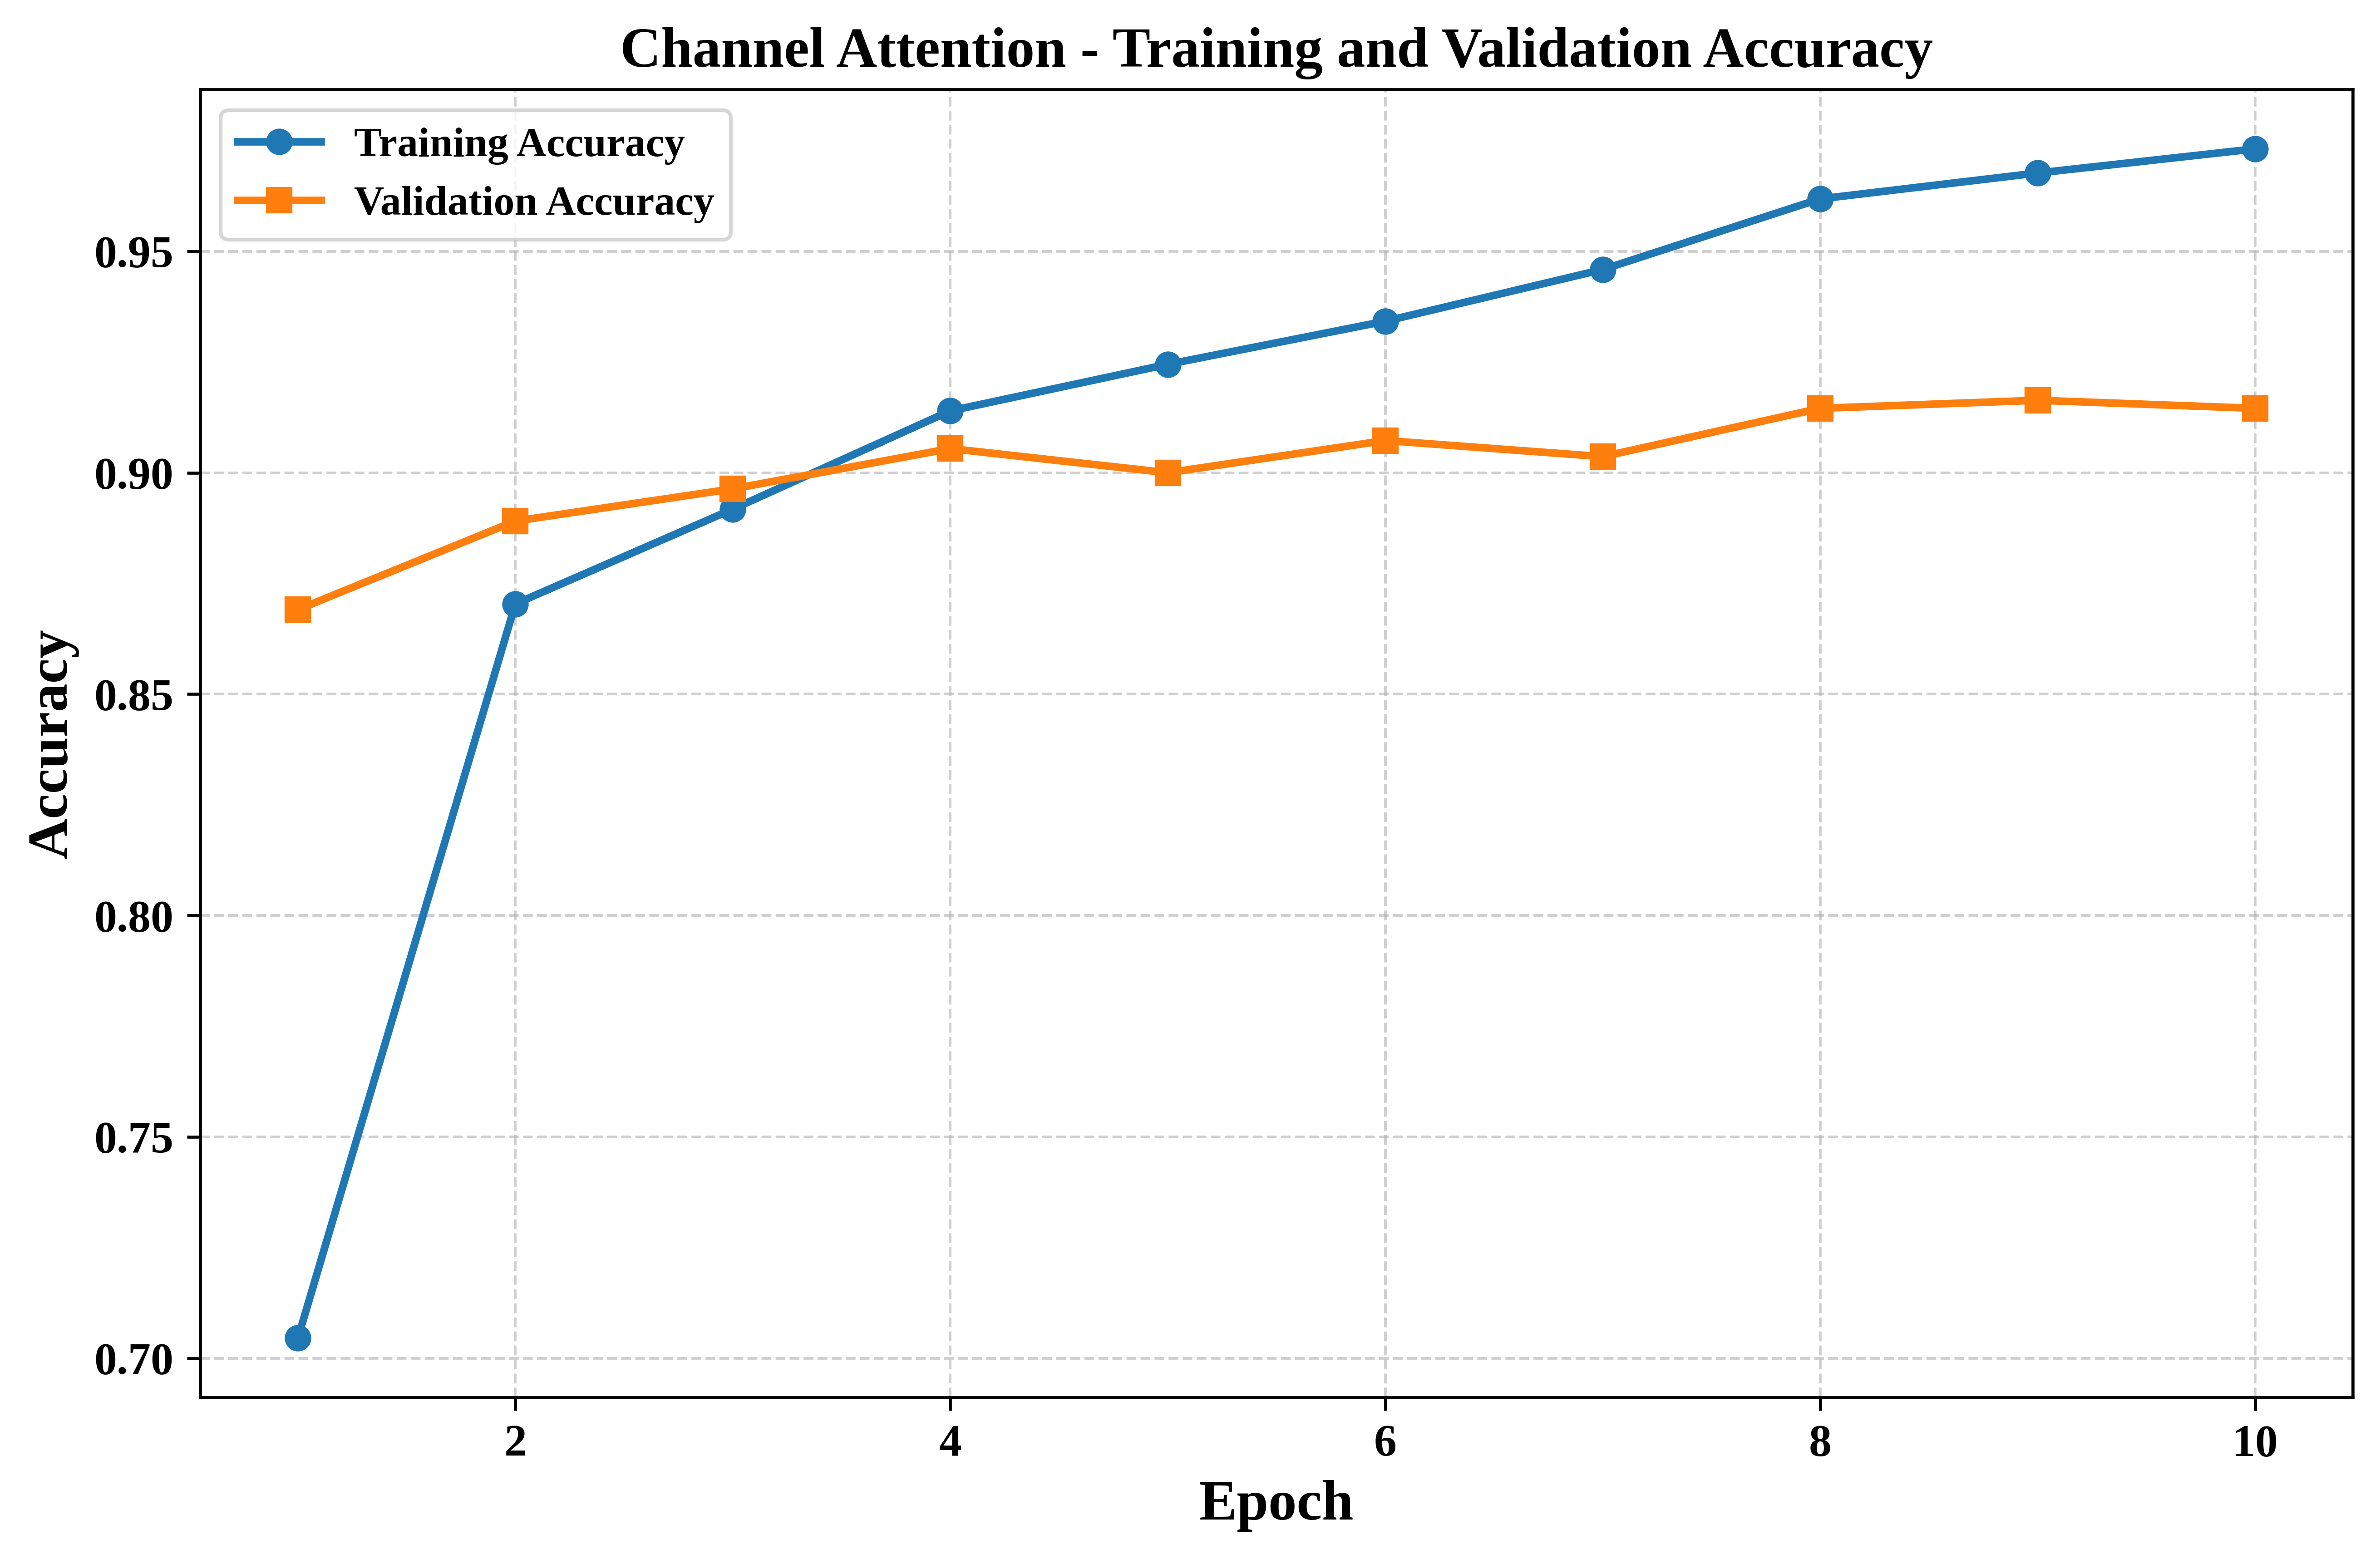
\includegraphics[width=\linewidth]{Images/use/exp1_attention_channel_accuracy.png}
    \caption{Training and Validation Accuracy}
\end{subfigure}
\hfill
\begin{subfigure}[b]{0.485\textwidth}
    \centering
    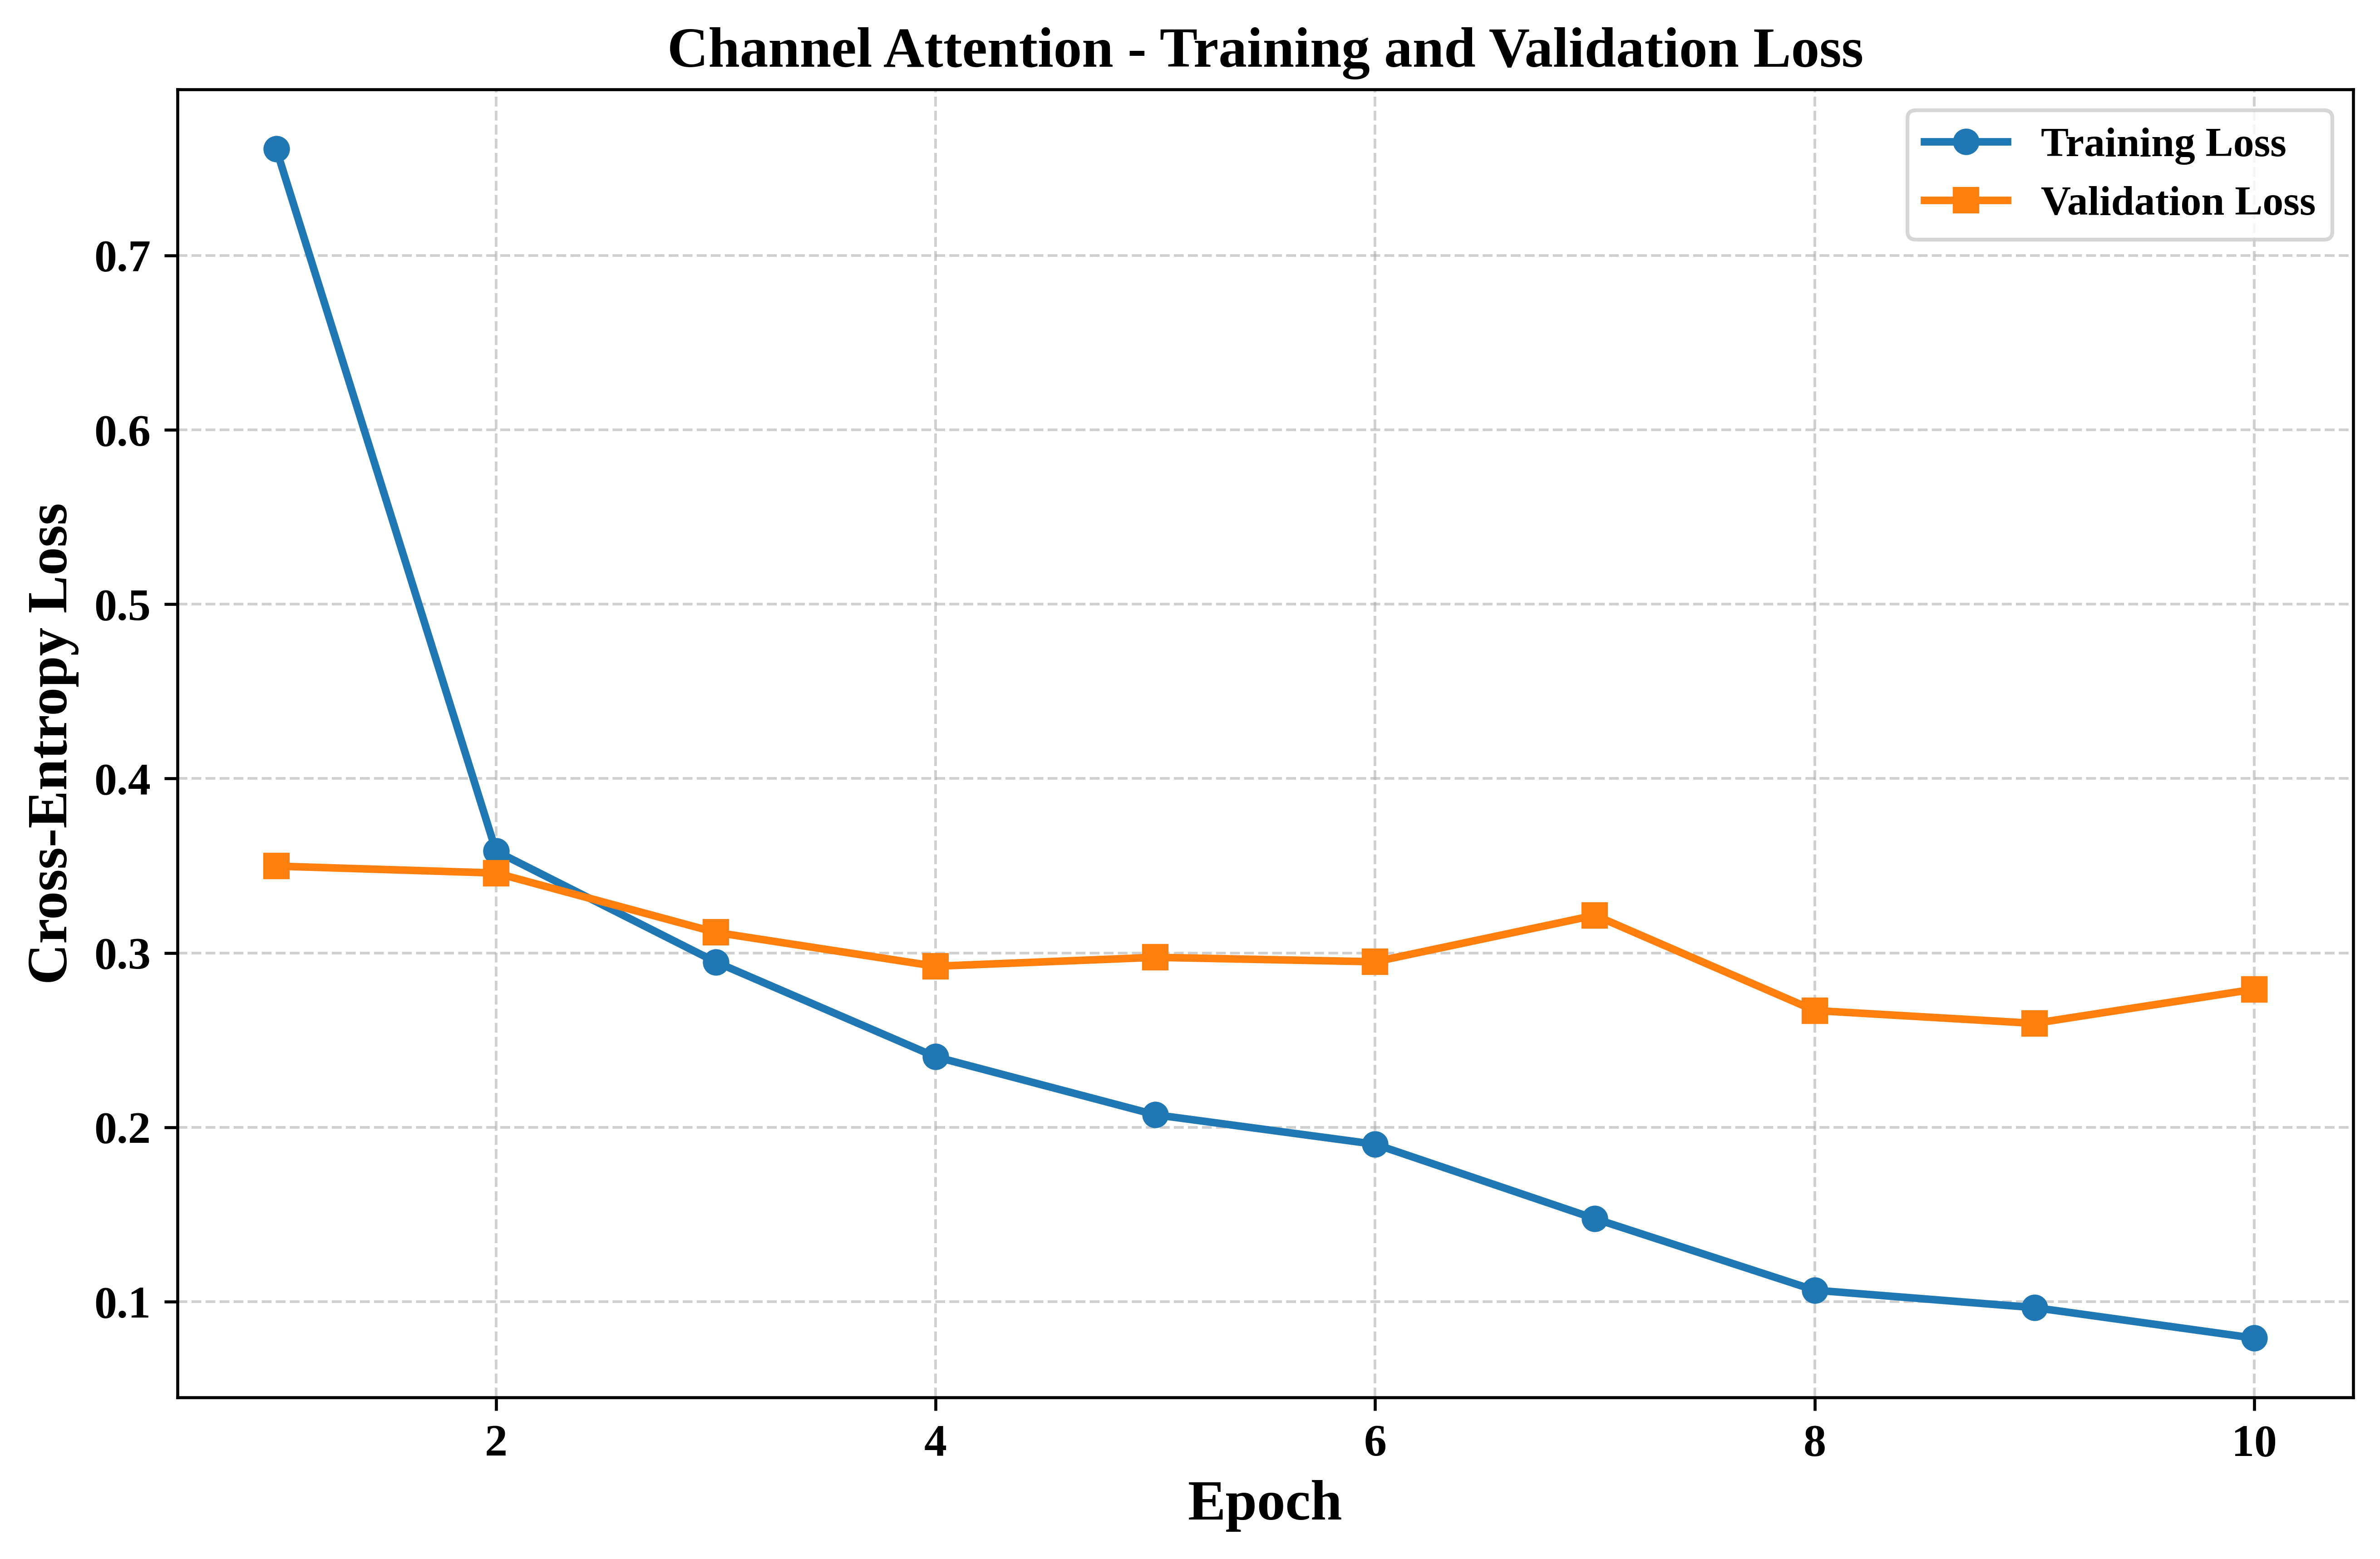
\includegraphics[width=\linewidth]{Images/use/exp1_attention_channel_loss.png}
    \caption{Training and Validation Loss}
\end{subfigure}

\vspace{2mm}
\begin{subfigure}[b]{0.44\textwidth}
    \centering
    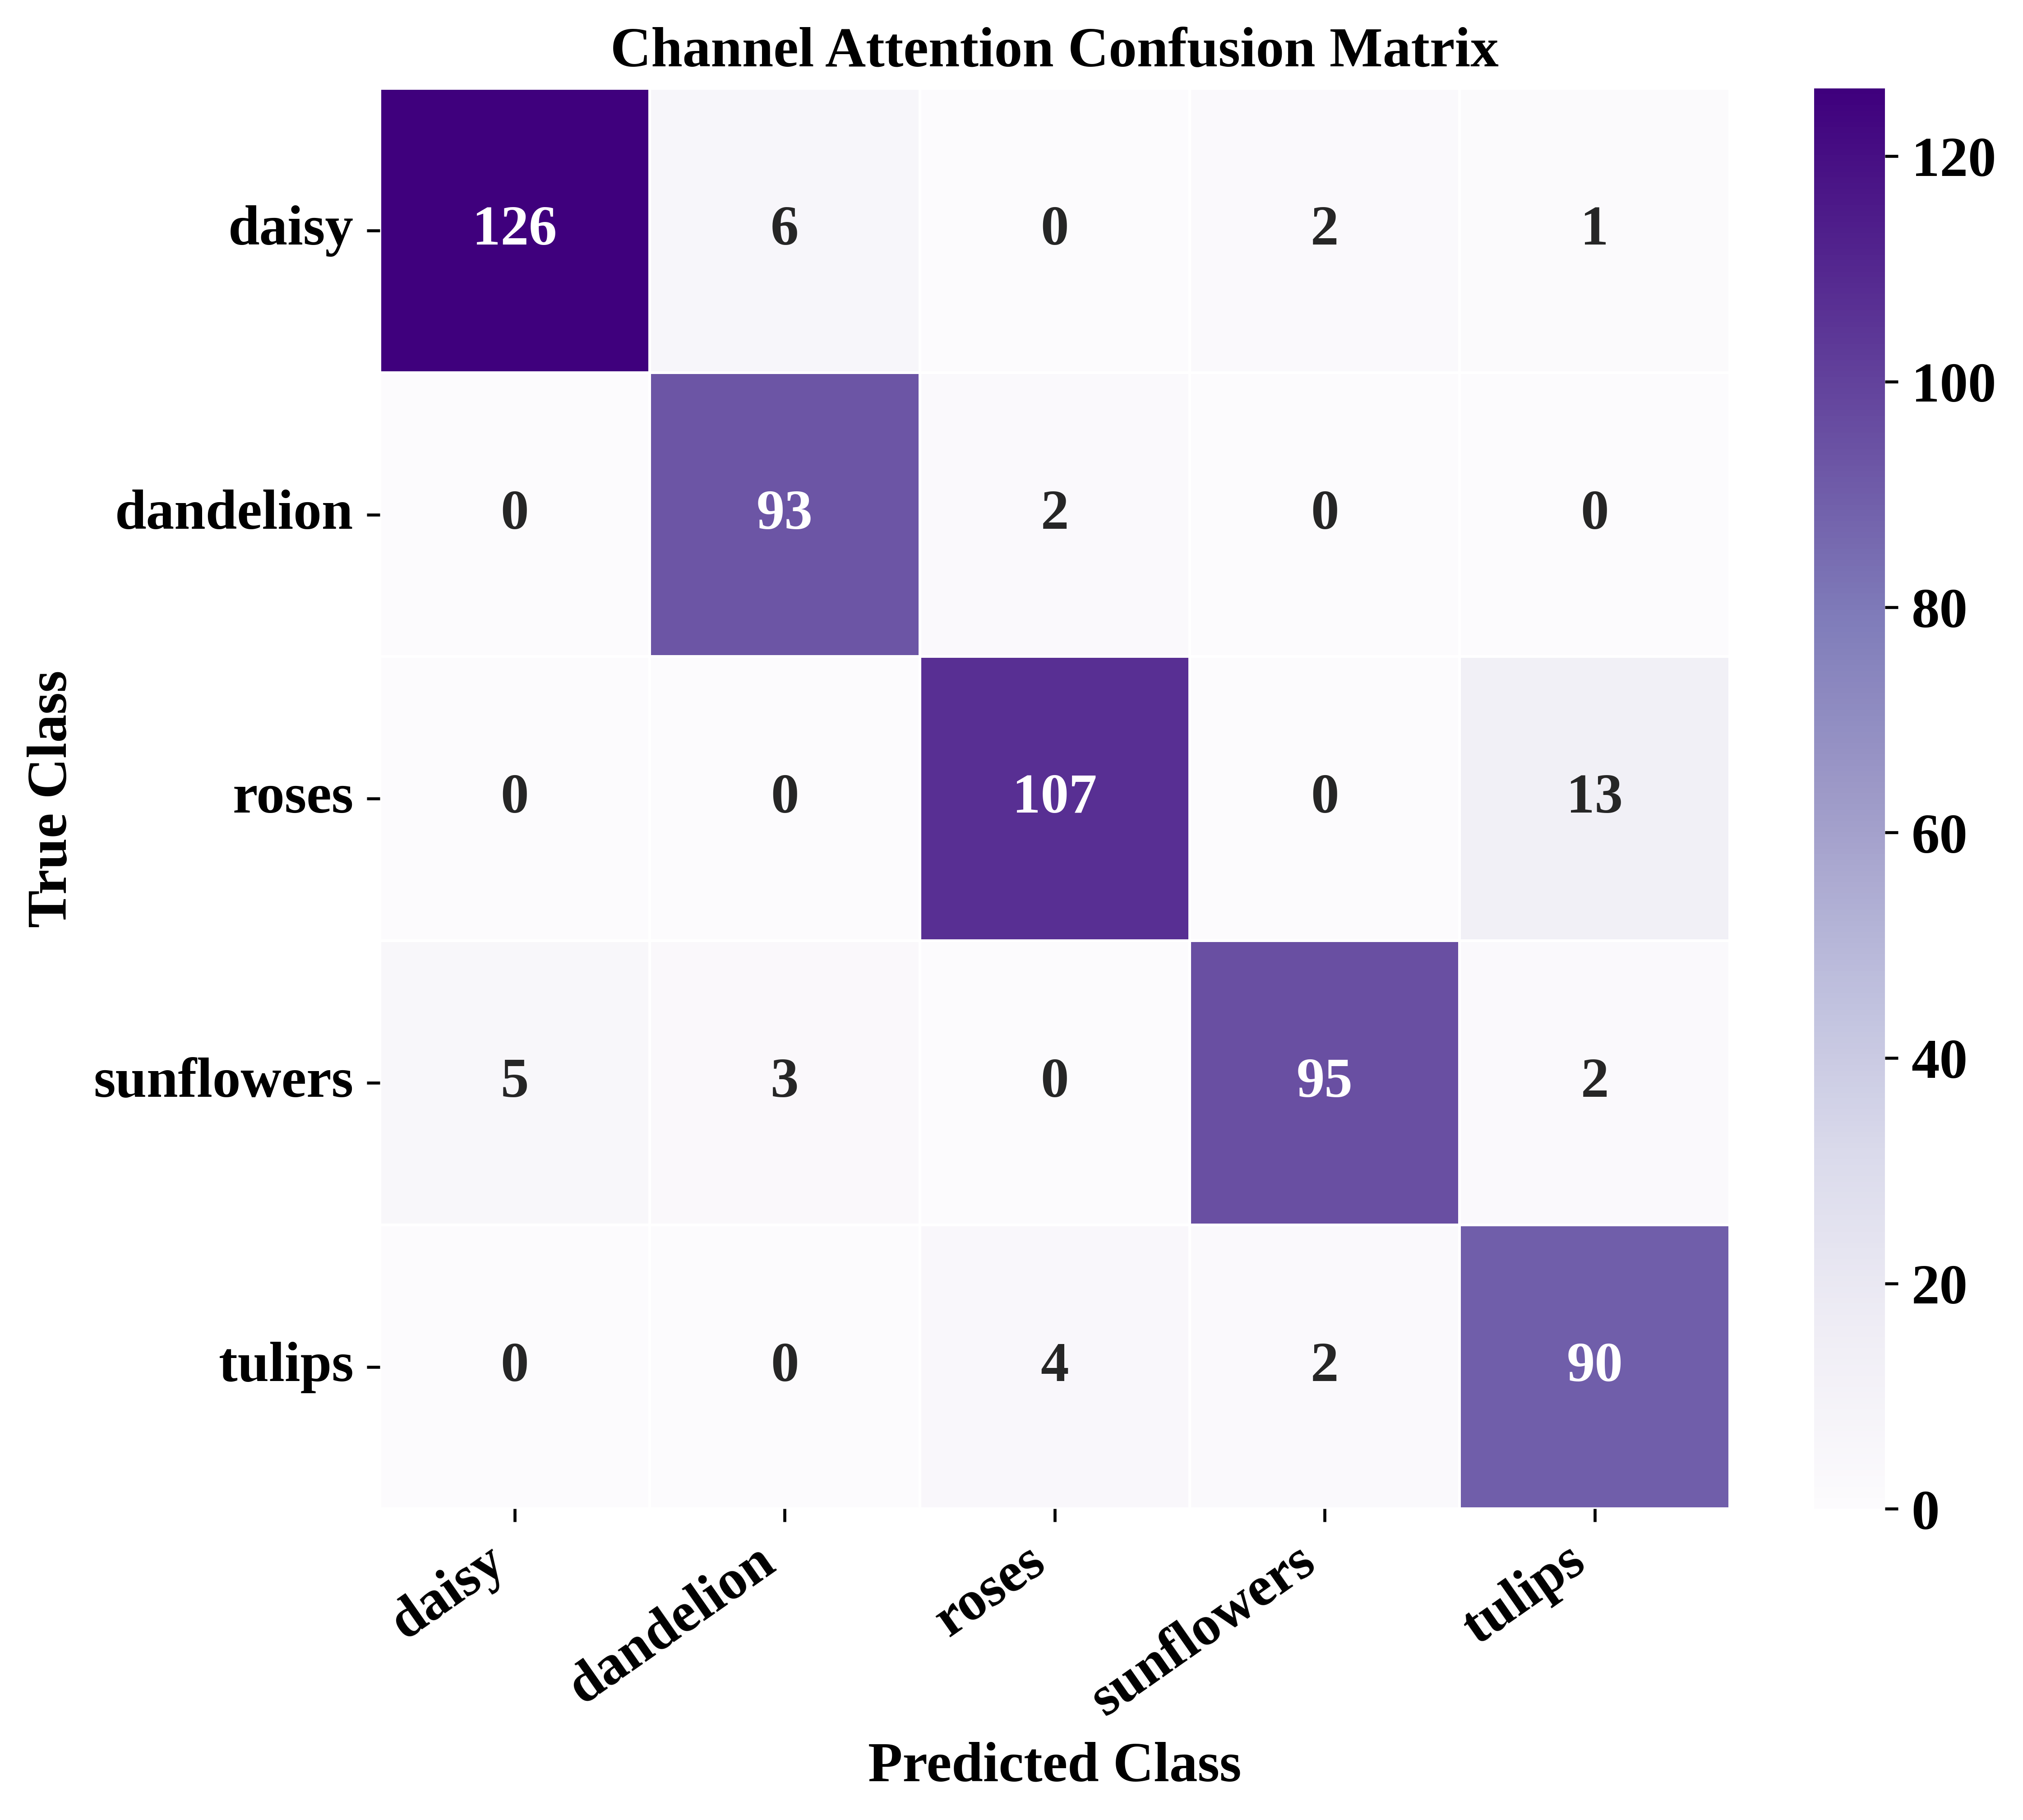
\includegraphics[width=\linewidth]{Images/use/exp1_attention_channel_confusion_matrix.png}
    \caption{Test Confusion Matrix}
\end{subfigure}
\caption{ResNet50 with Channel Attention at stage $P_3$ (conv4\_x): Training and validation accuracy trajectories, loss convergence, and test confusion matrix.}
\label{fig:channel_group}
\end{figure}

\textbf{Inference:}  Inclusion of channel attention at stage $P_3$ dynamically recalibrates the response of channel-wise features, thus achieving the validation accuracy of about 92.4\% and speeding up loss minimization to 0.22. By learning interdependencies among channels through squeeze-and-excitation pooling, the network enhances discriminative feature detectors and suppresses background features. As a result, test misclassification of neighboring categories such as roses and tulips is significantly reduced, which means that channel recalibration improves category-specific semantic separation.

\vspace{3mm}

% ------------------------------------------------------------
\subsection*{30.4 Spatial Attention ($k=5$) at $P_3$ (conv4\_x): Accuracy, Loss, and Confusion Matrix}
% ------------------------------------------------------------

\begin{figure}[H]
\centering
\begin{subfigure}[b]{0.485\textwidth}
    \centering
    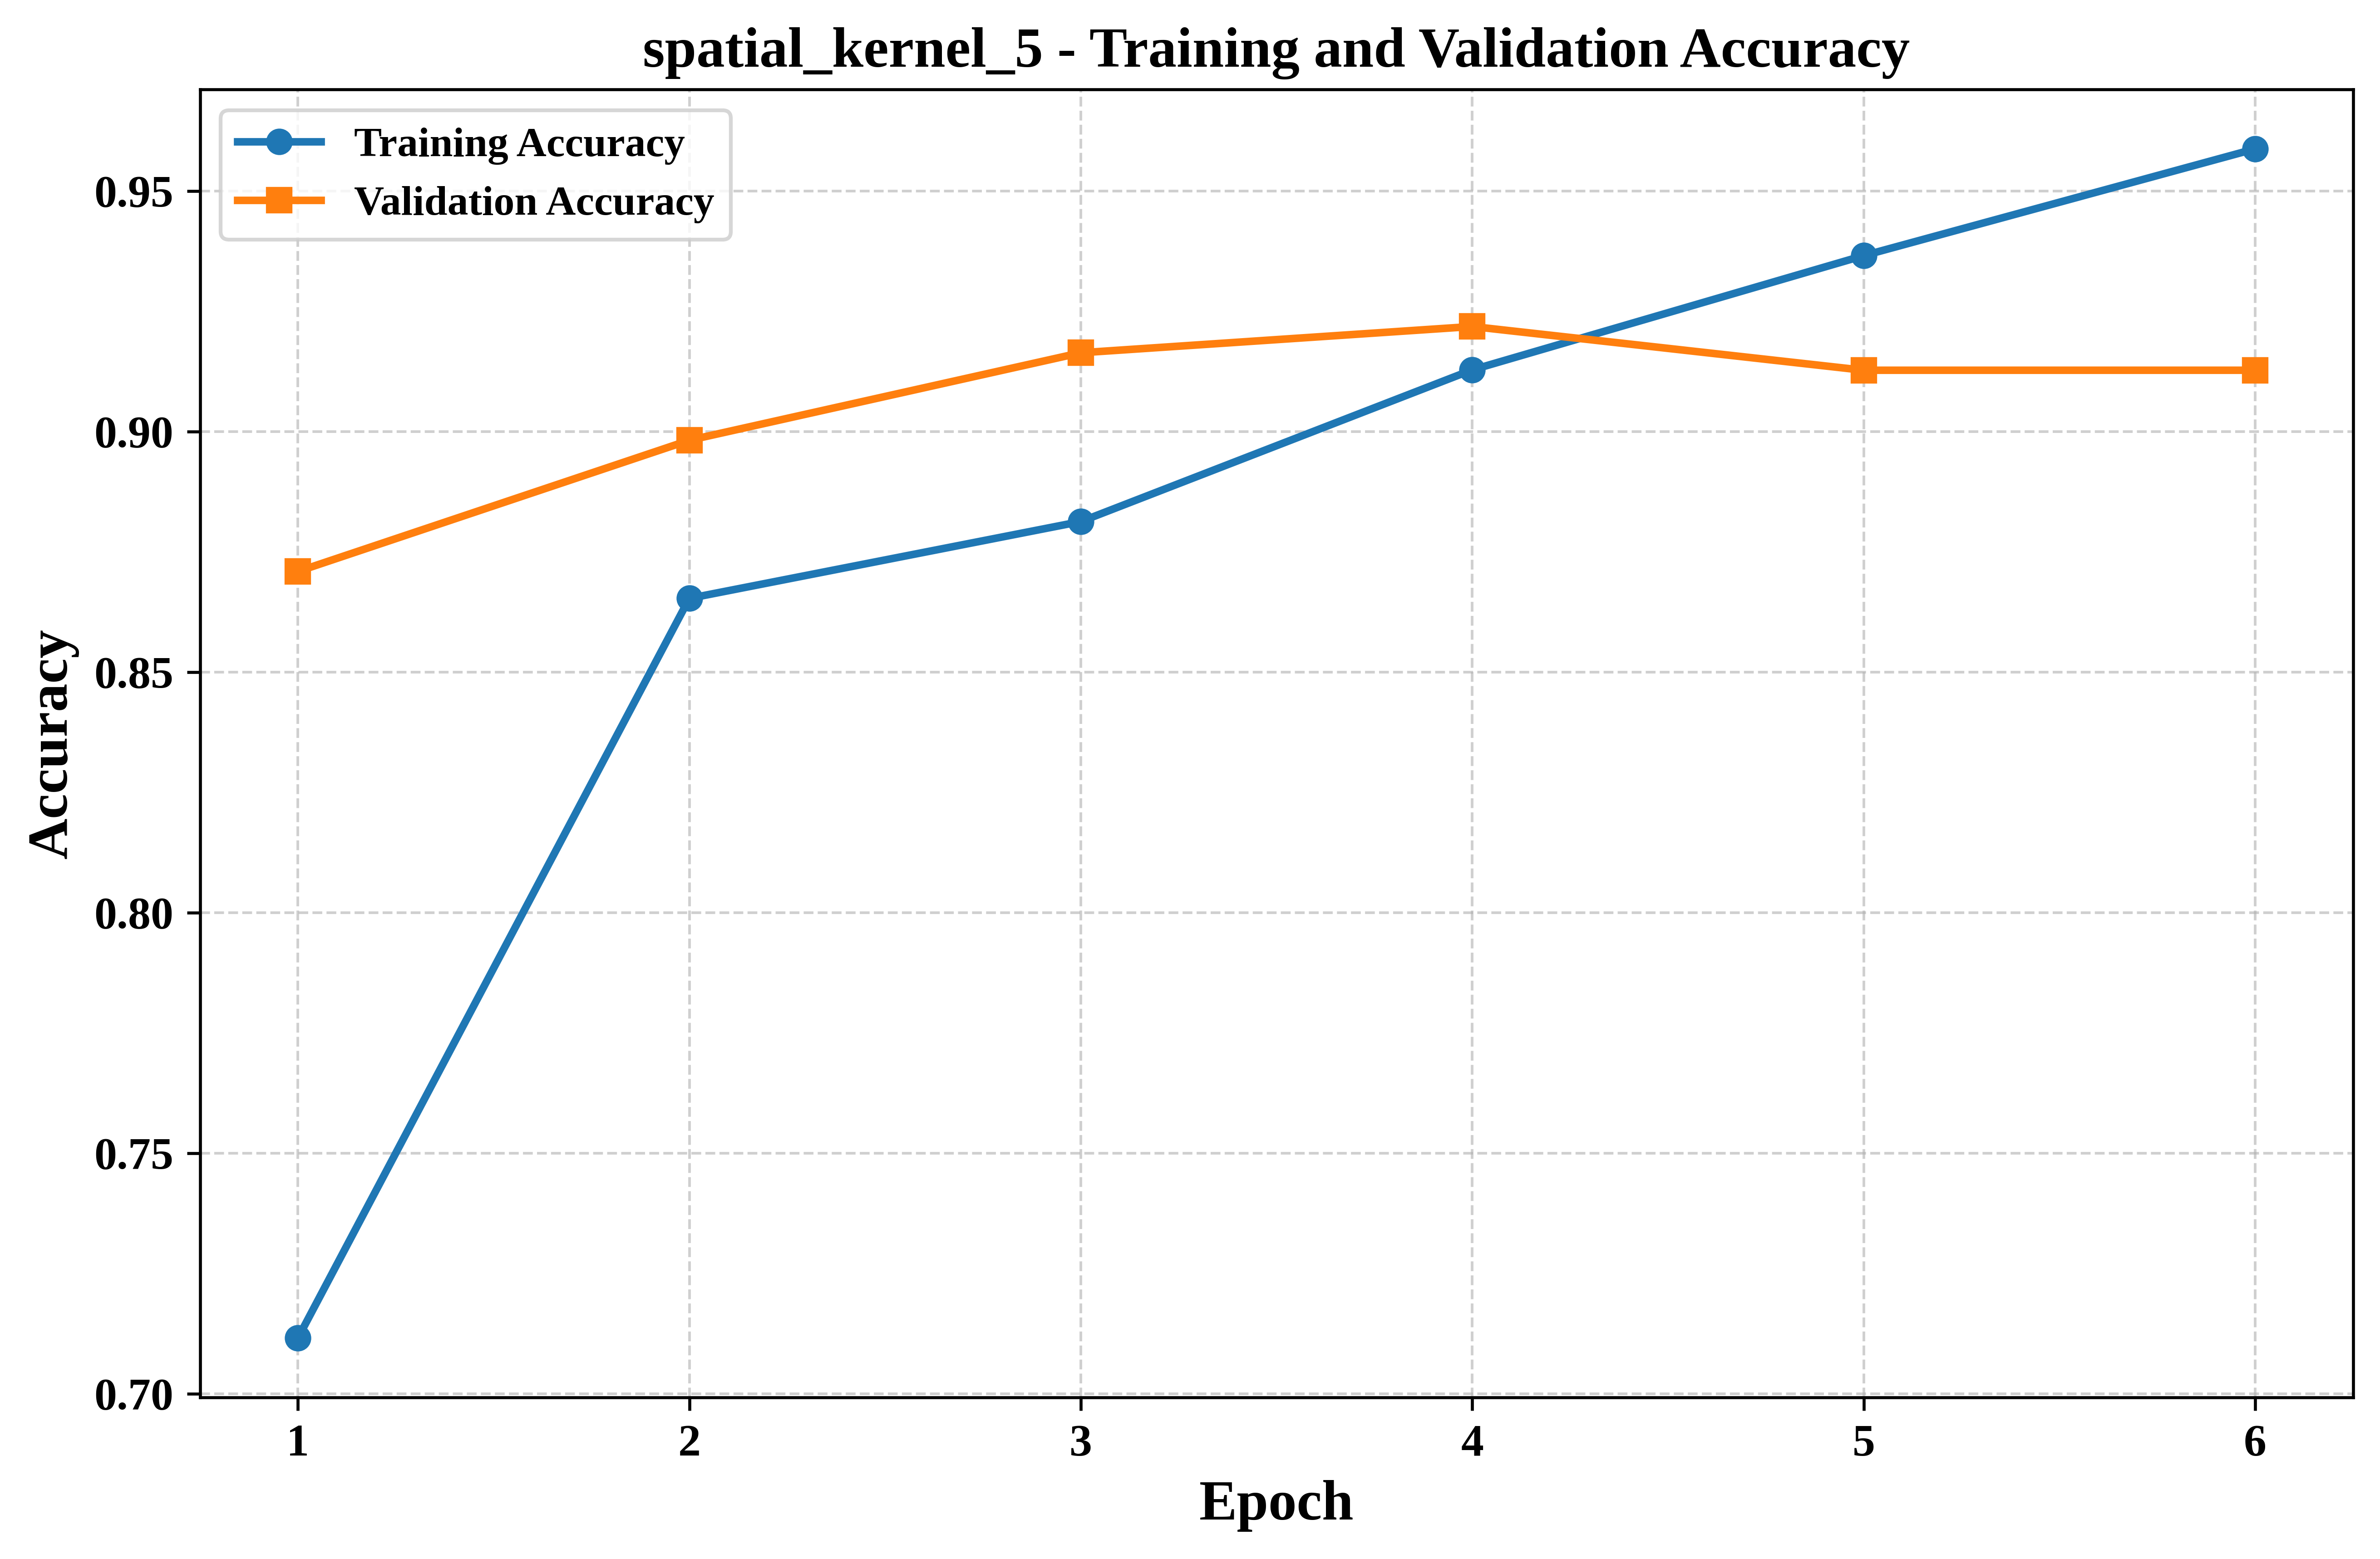
\includegraphics[width=\linewidth]{Images/use/spatial_kernel_5_accuracy.png}
    \caption{Training and Validation Accuracy}
\end{subfigure}
\hfill
\begin{subfigure}[b]{0.485\textwidth}
    \centering
    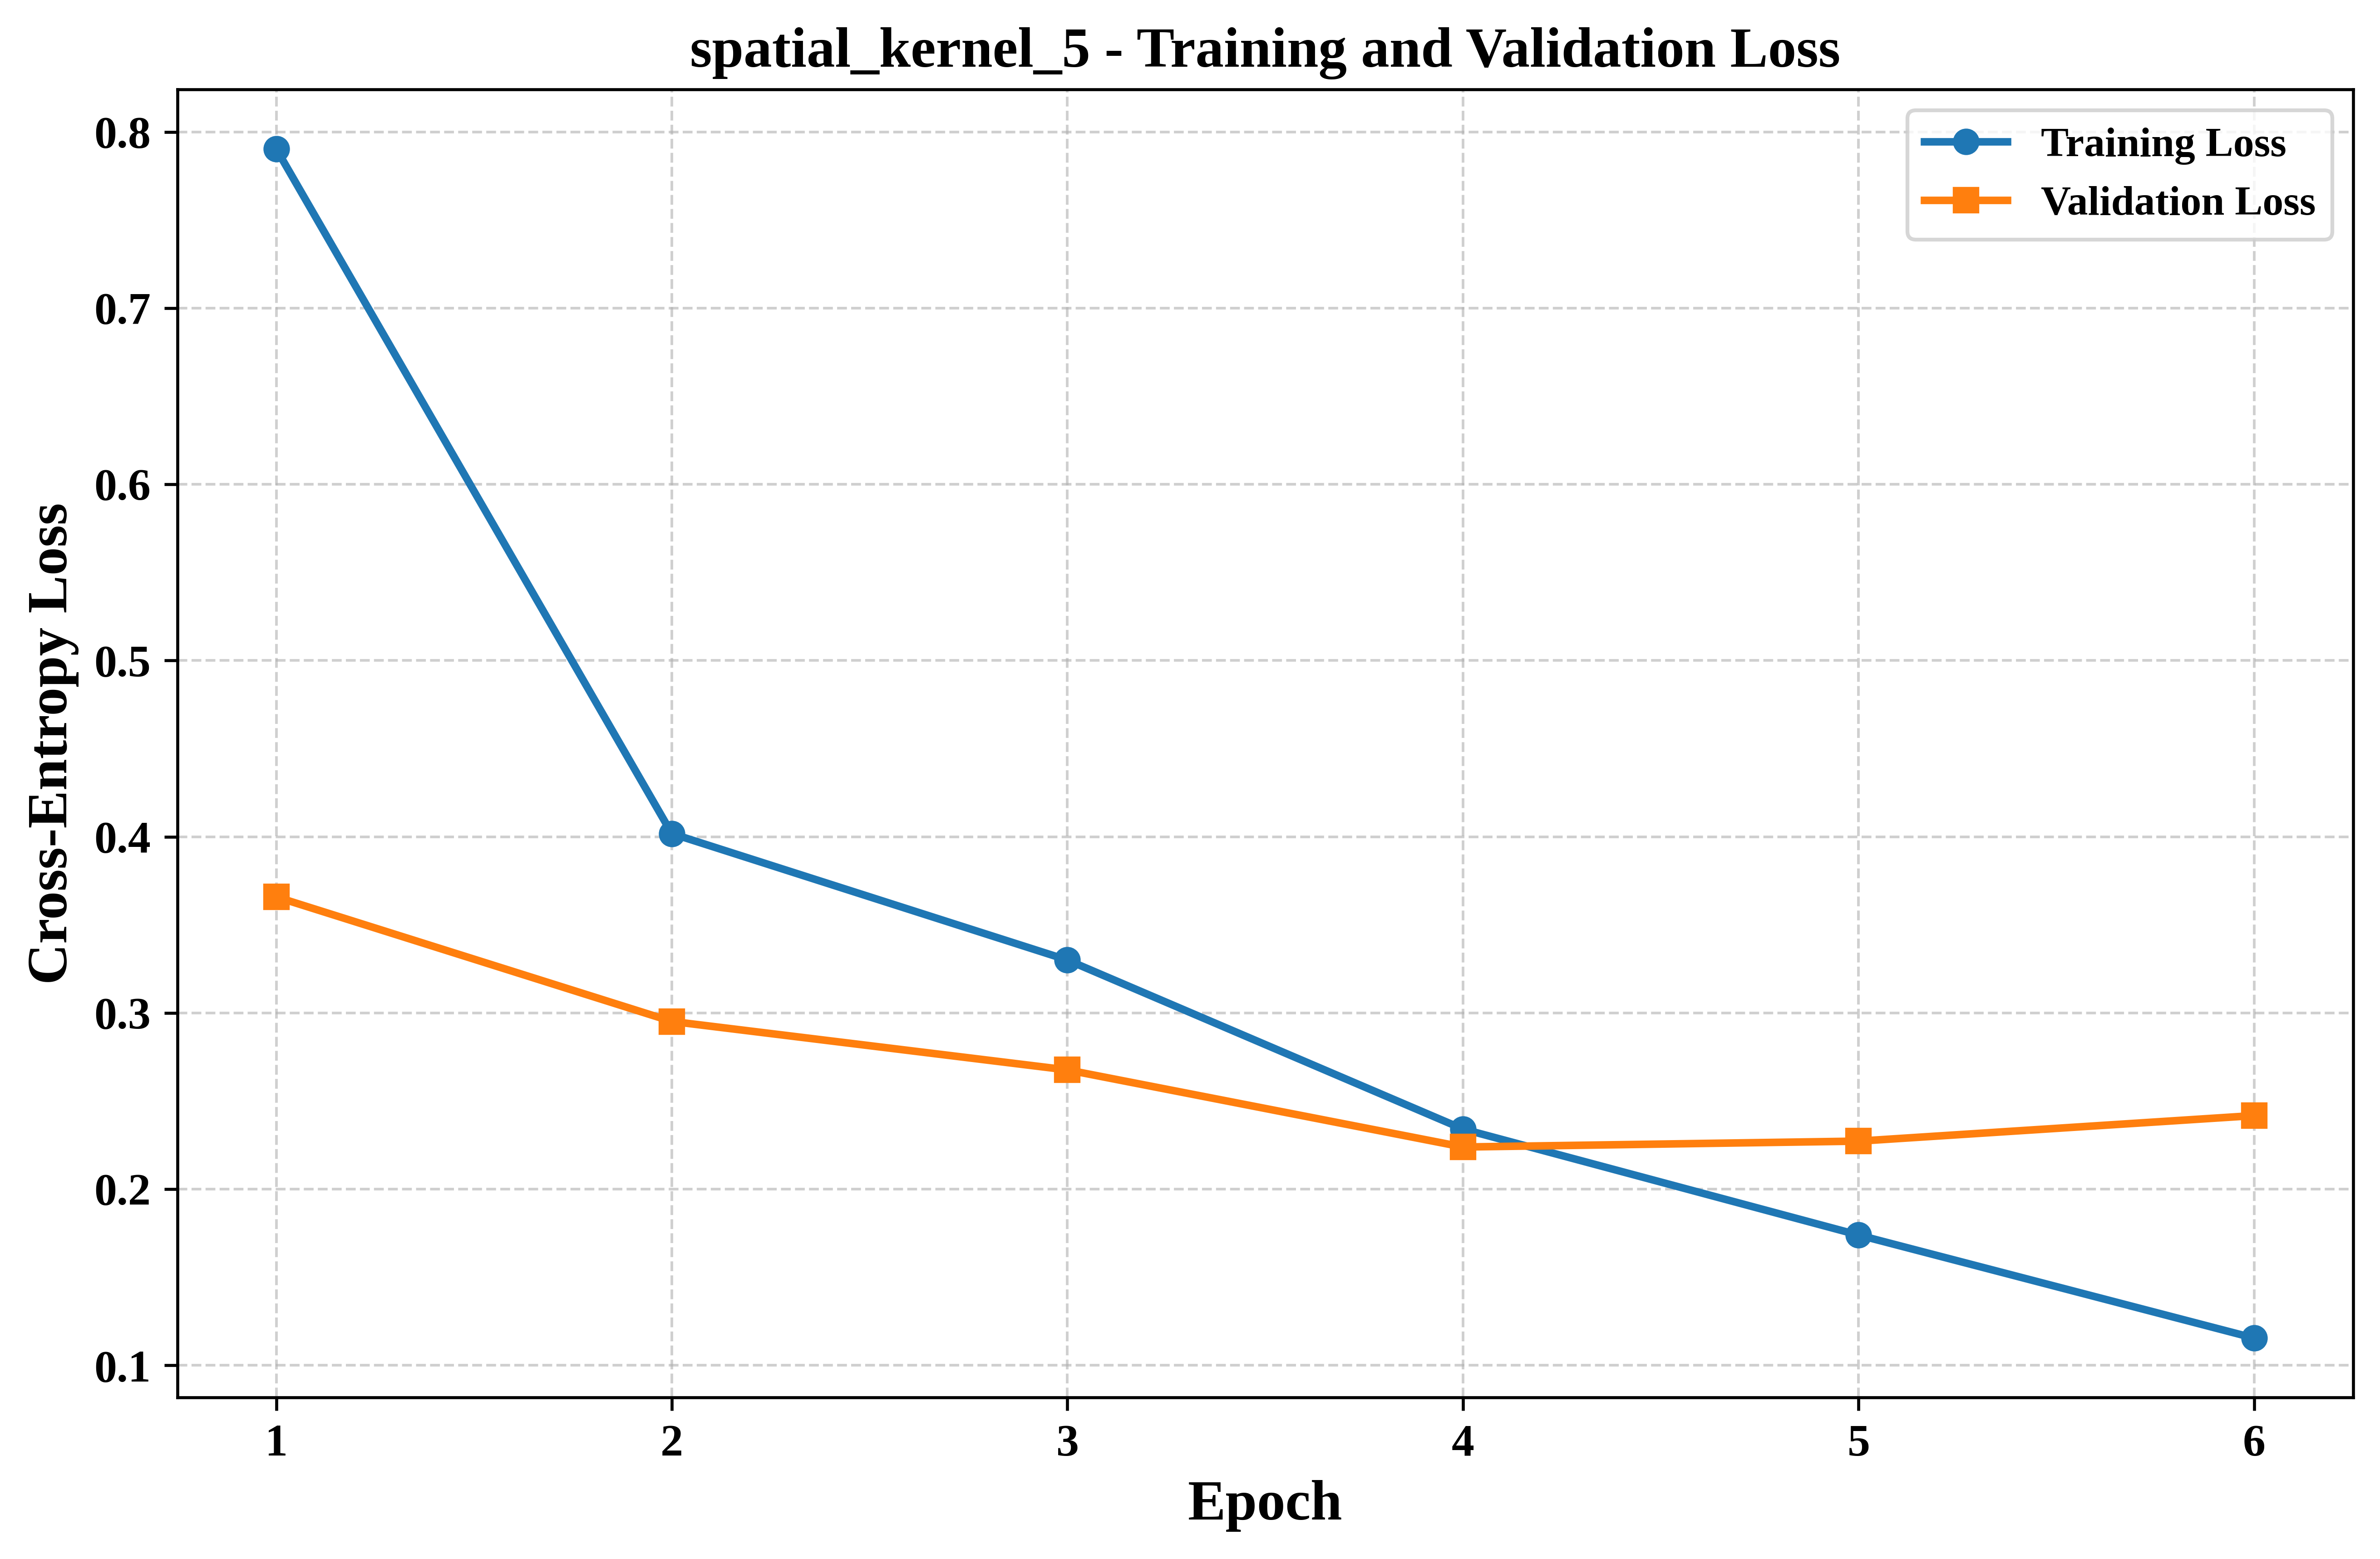
\includegraphics[width=\linewidth]{Images/use/spatial_kernel_5_loss.png}
    \caption{Training and Validation Loss}
\end{subfigure}

\vspace{2mm}
\begin{subfigure}[b]{0.44\textwidth}
    \centering
    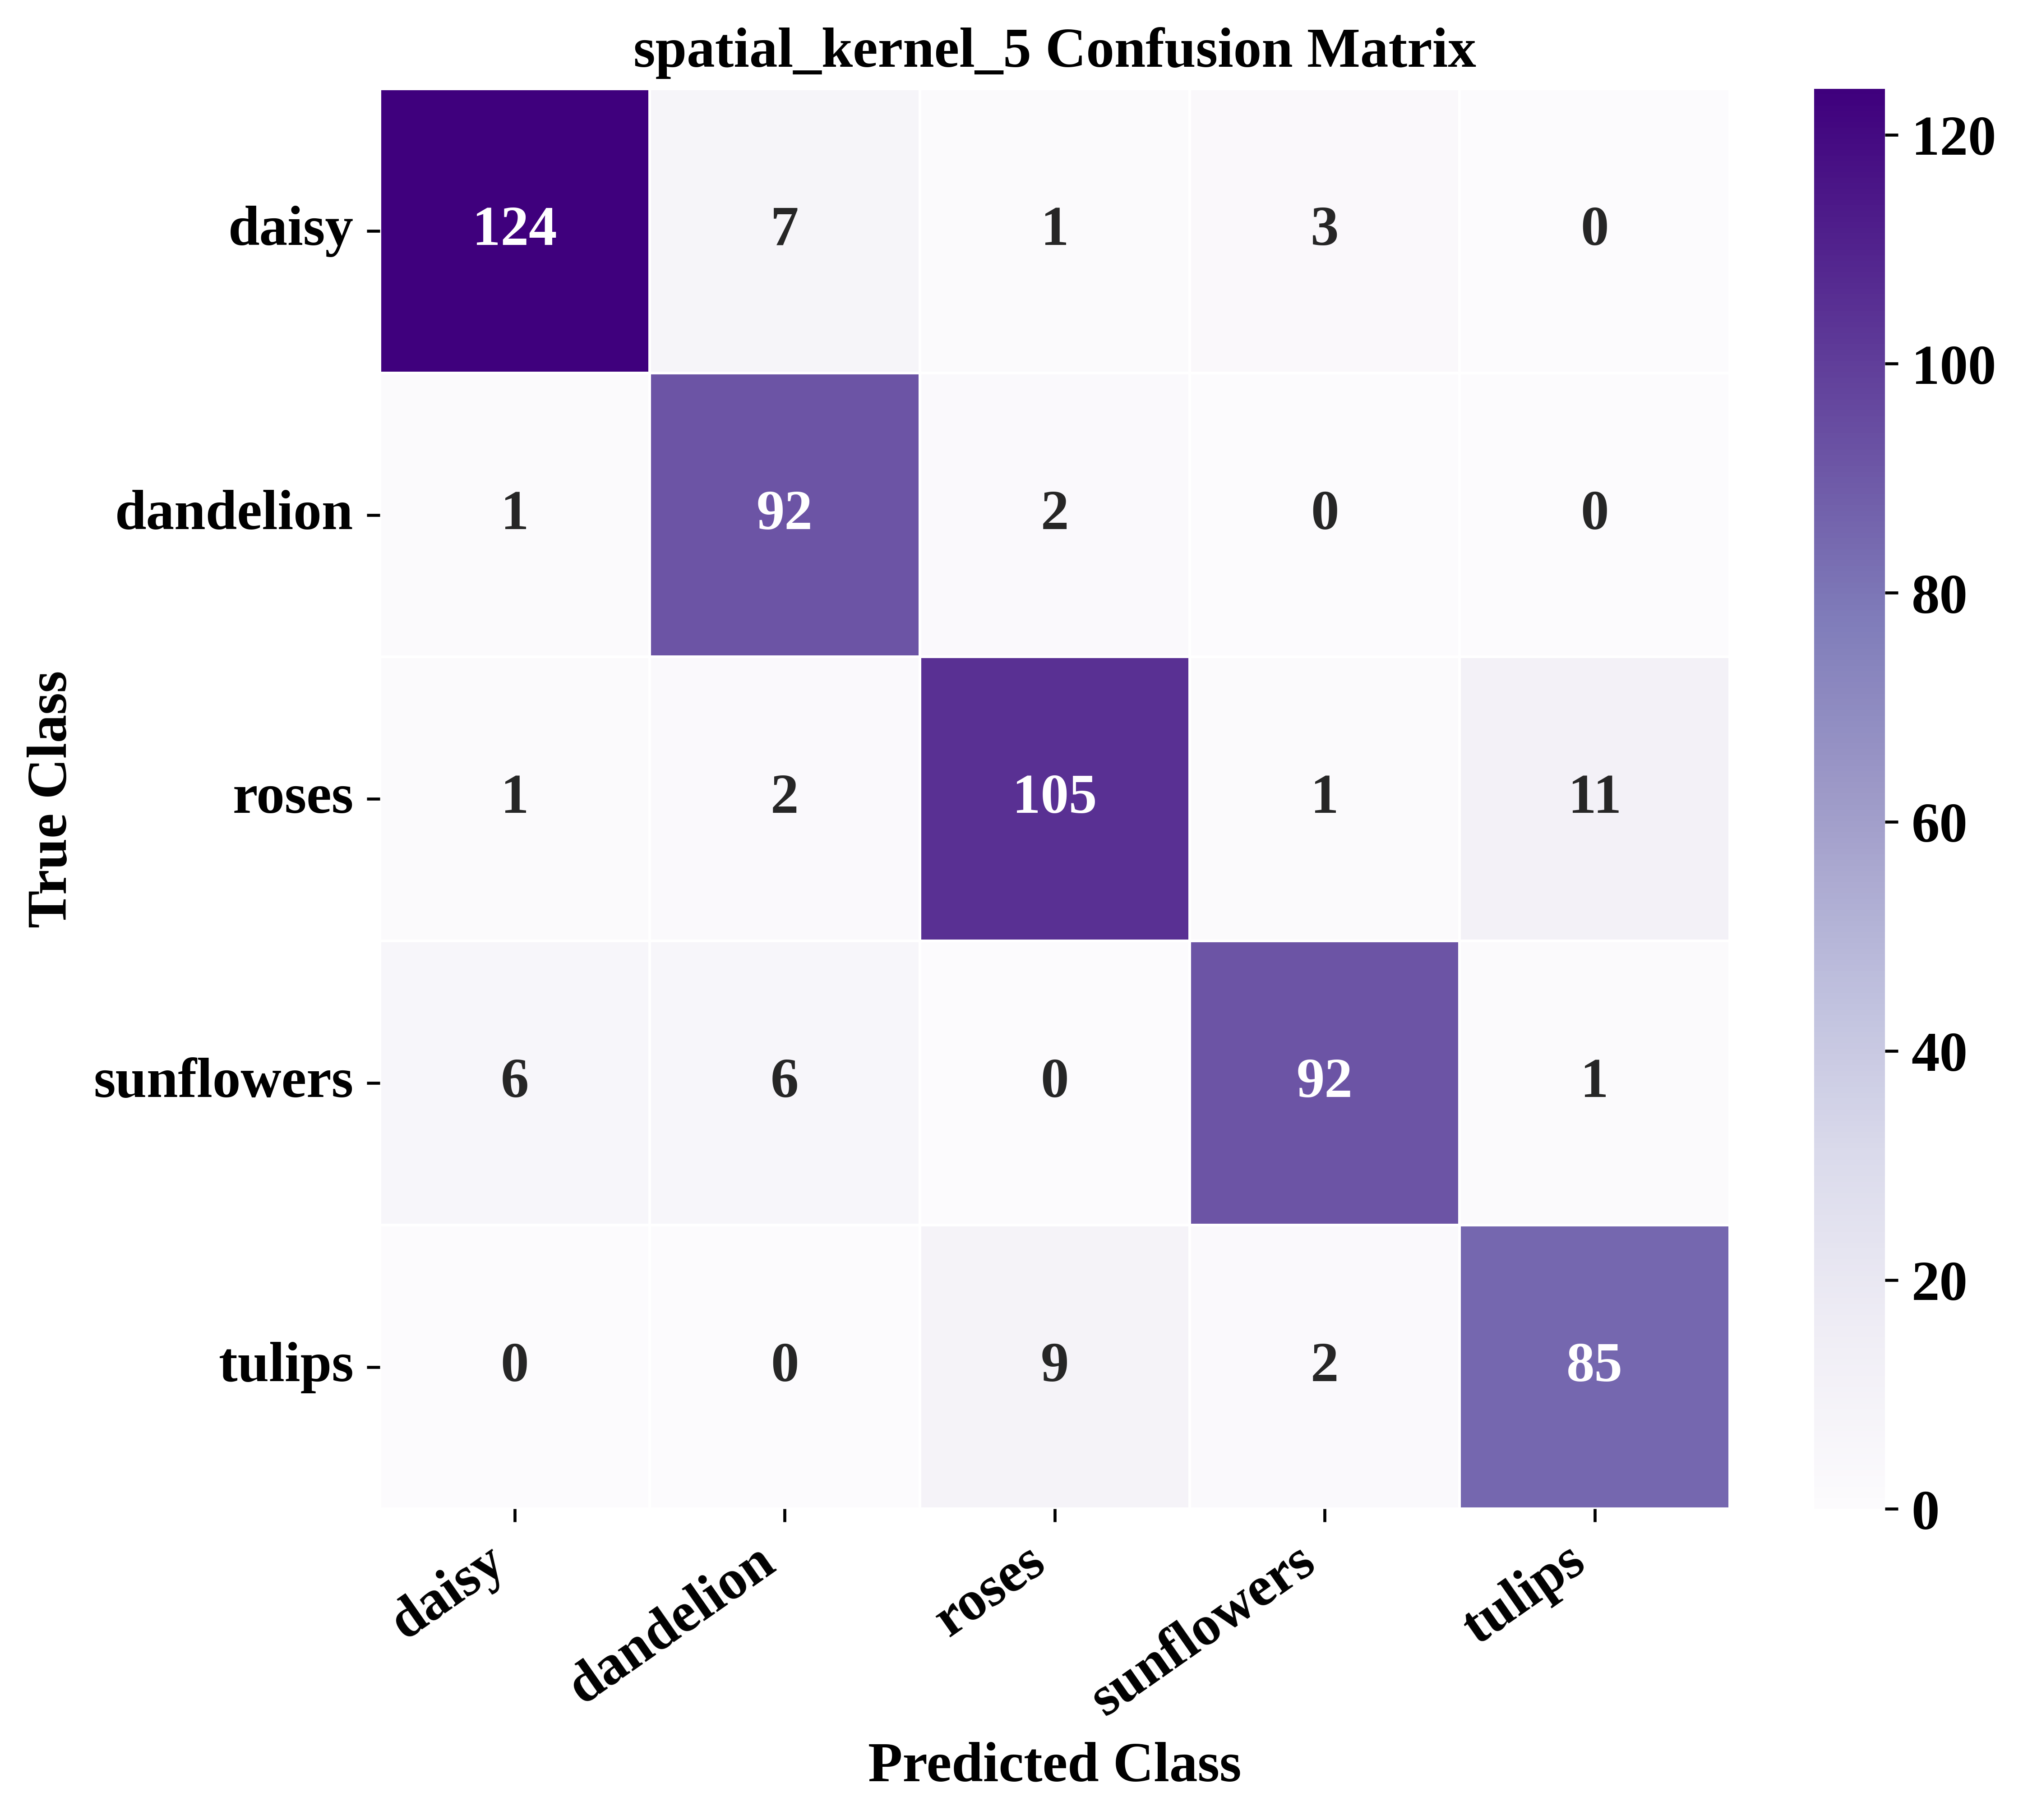
\includegraphics[width=\linewidth]{Images/use/spatial_kernel_5_confusion_matrix.png}
    \caption{Test Confusion Matrix}
\end{subfigure}
\caption{ResNet50 with Spatial Attention ($k=5$) at stage $P_3$: Training and validation accuracy curves, cross-entropy loss progression, and test confusion matrix.}
\label{fig:spatial_group}
\end{figure}

\textbf{Inference:} 
Application of spatial attention using $5 \times 5$ convolution kernel at stage $P_3$ results in good convergence with validation accuracy achieving ~91.8\% and the cross-entropy loss of 0.24. The spatial attention layer calculates statistics of channels to generate a two-dimensional saliency map for guiding further convolution filters toward contrastive flower heads. According to the confusion matrix, accuracy on sunflowers and daisies has been enhanced by this method, thus demonstrating that intermediate spatial masking helps filter out irrelevant background features such as grass and sky.

\vspace{3mm}

% ------------------------------------------------------------
\subsection*{30.5 Squeeze-and-Excitation (SE) Attention at $P_3$: Accuracy, Loss, and Confusion Matrix}
% ------------------------------------------------------------

\begin{figure}[H]
\centering
\begin{subfigure}[b]{0.485\textwidth}
    \centering
    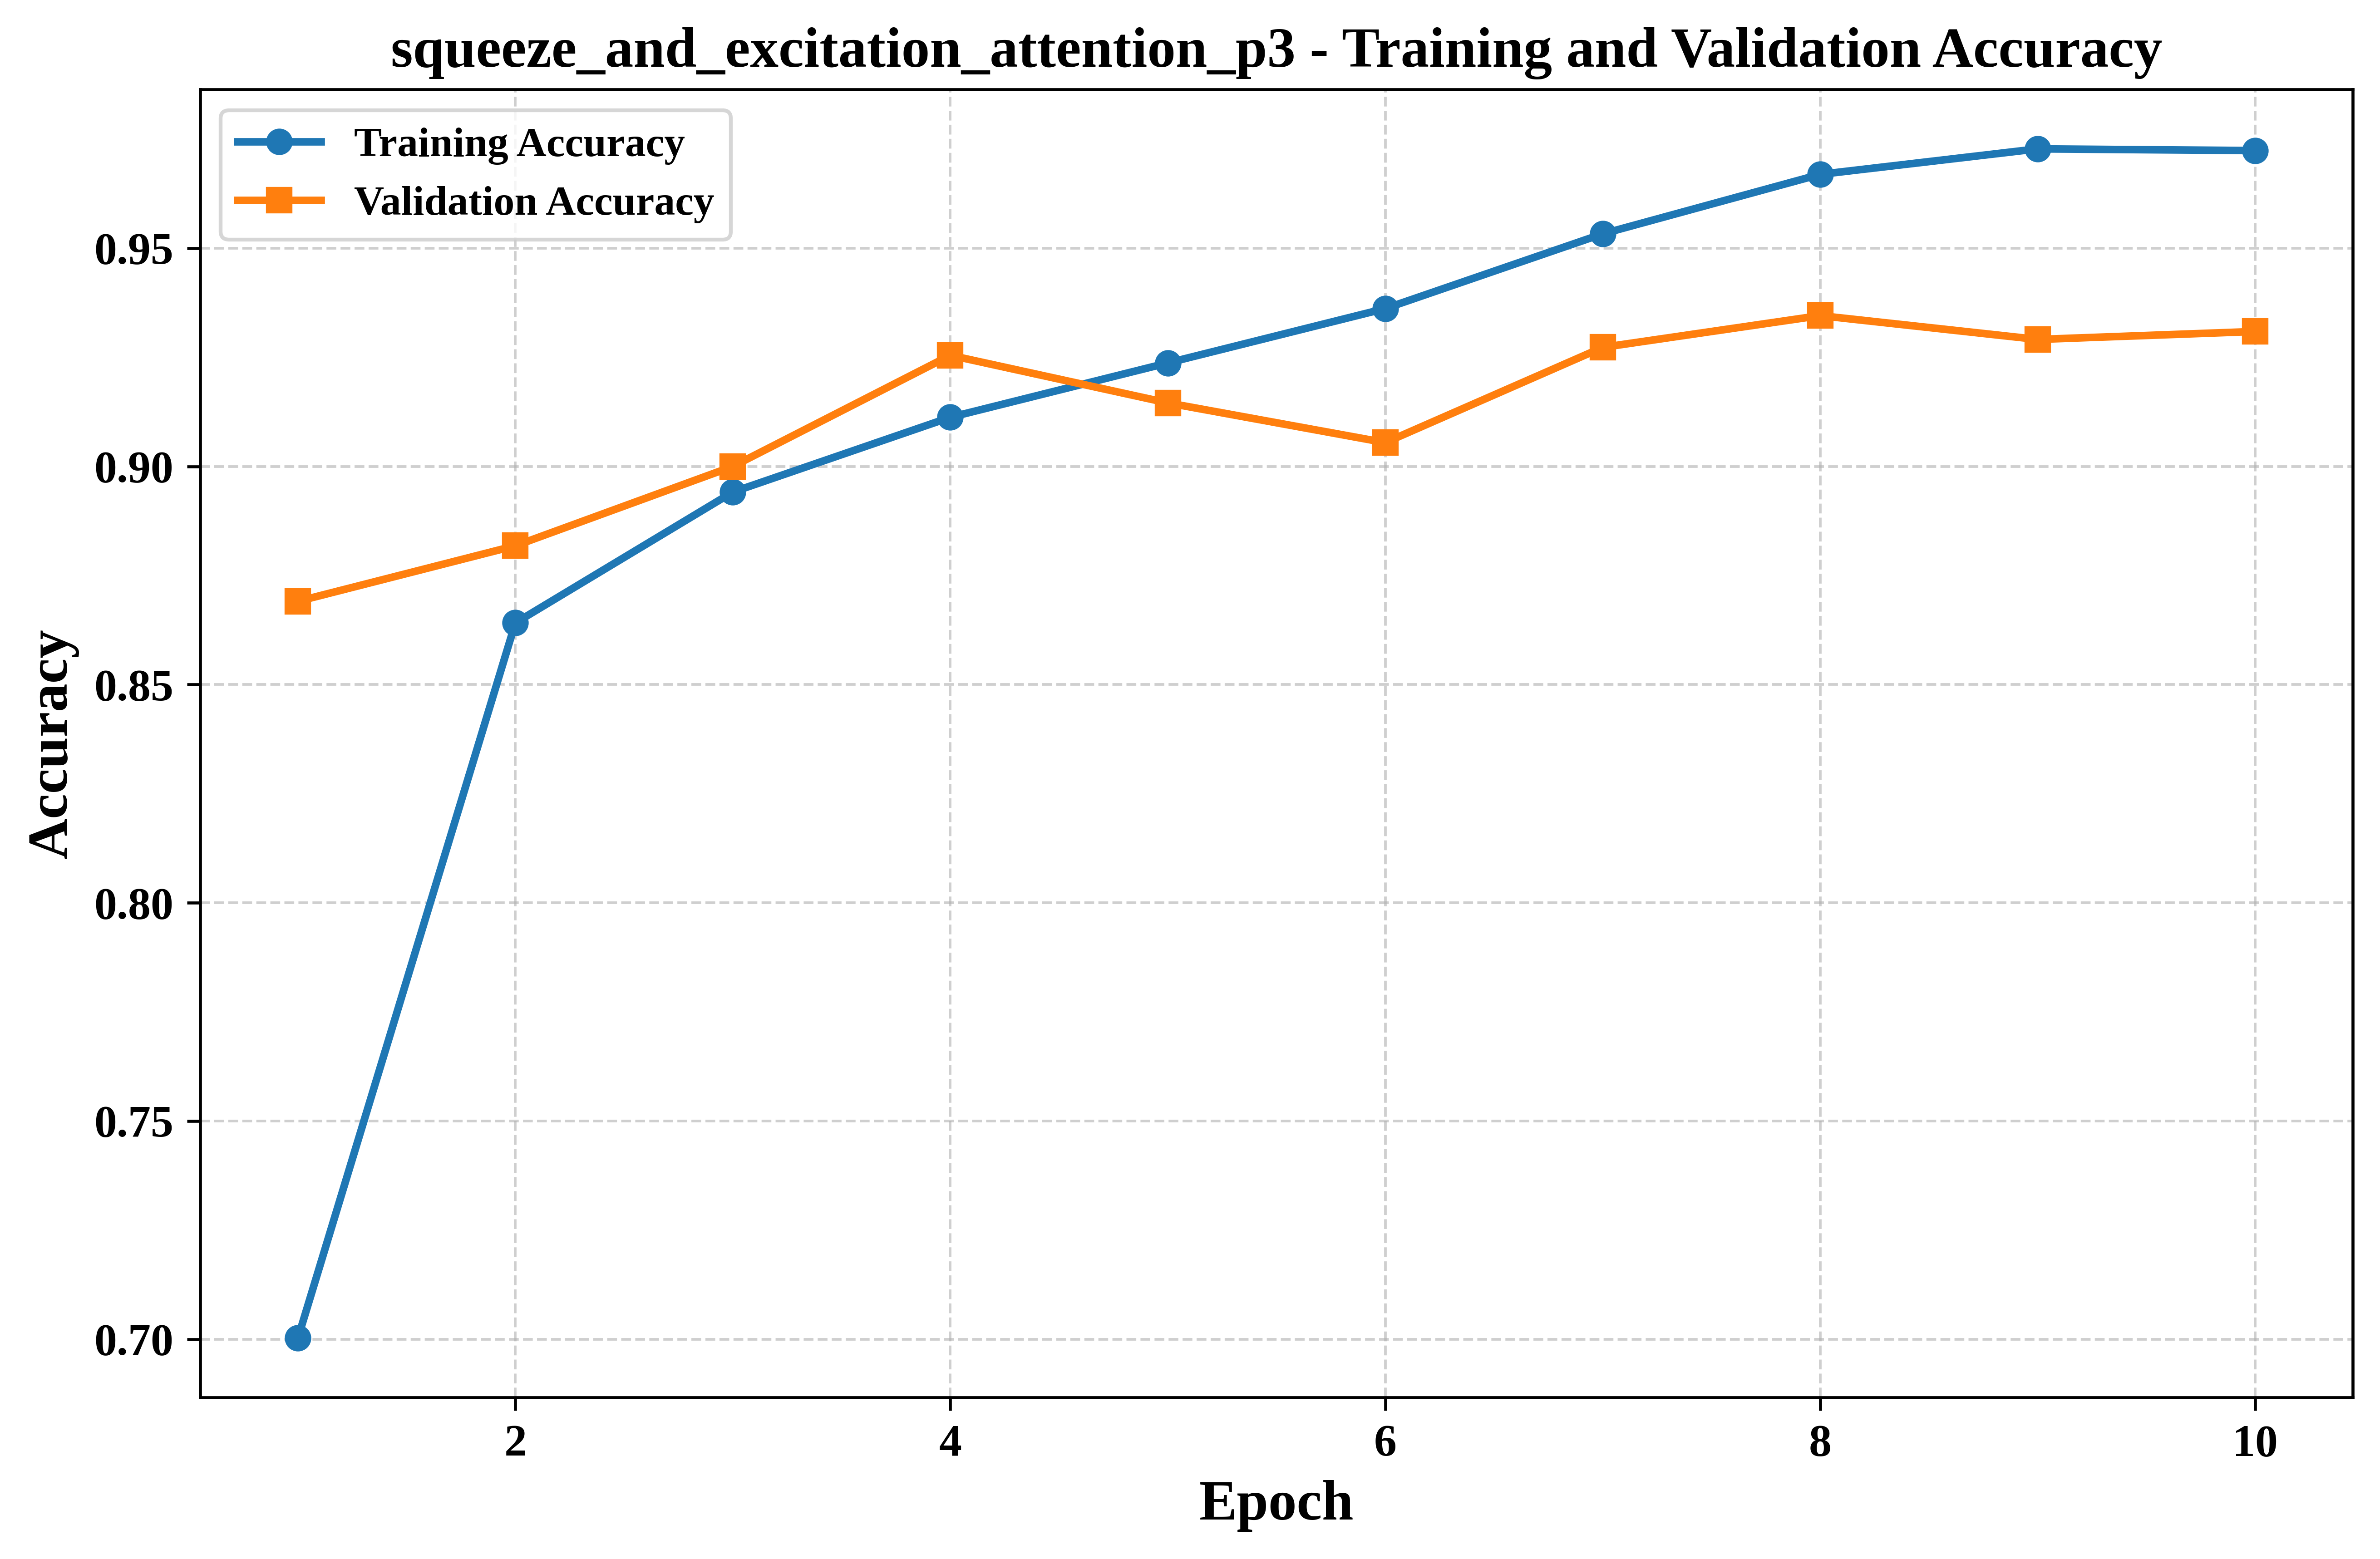
\includegraphics[width=\linewidth]{Images/use/squeeze_and_excitation_attention_p3_accuracy.png}
    \caption{Training and Validation Accuracy}
\end{subfigure}
\hfill
\begin{subfigure}[b]{0.485\textwidth}
    \centering
    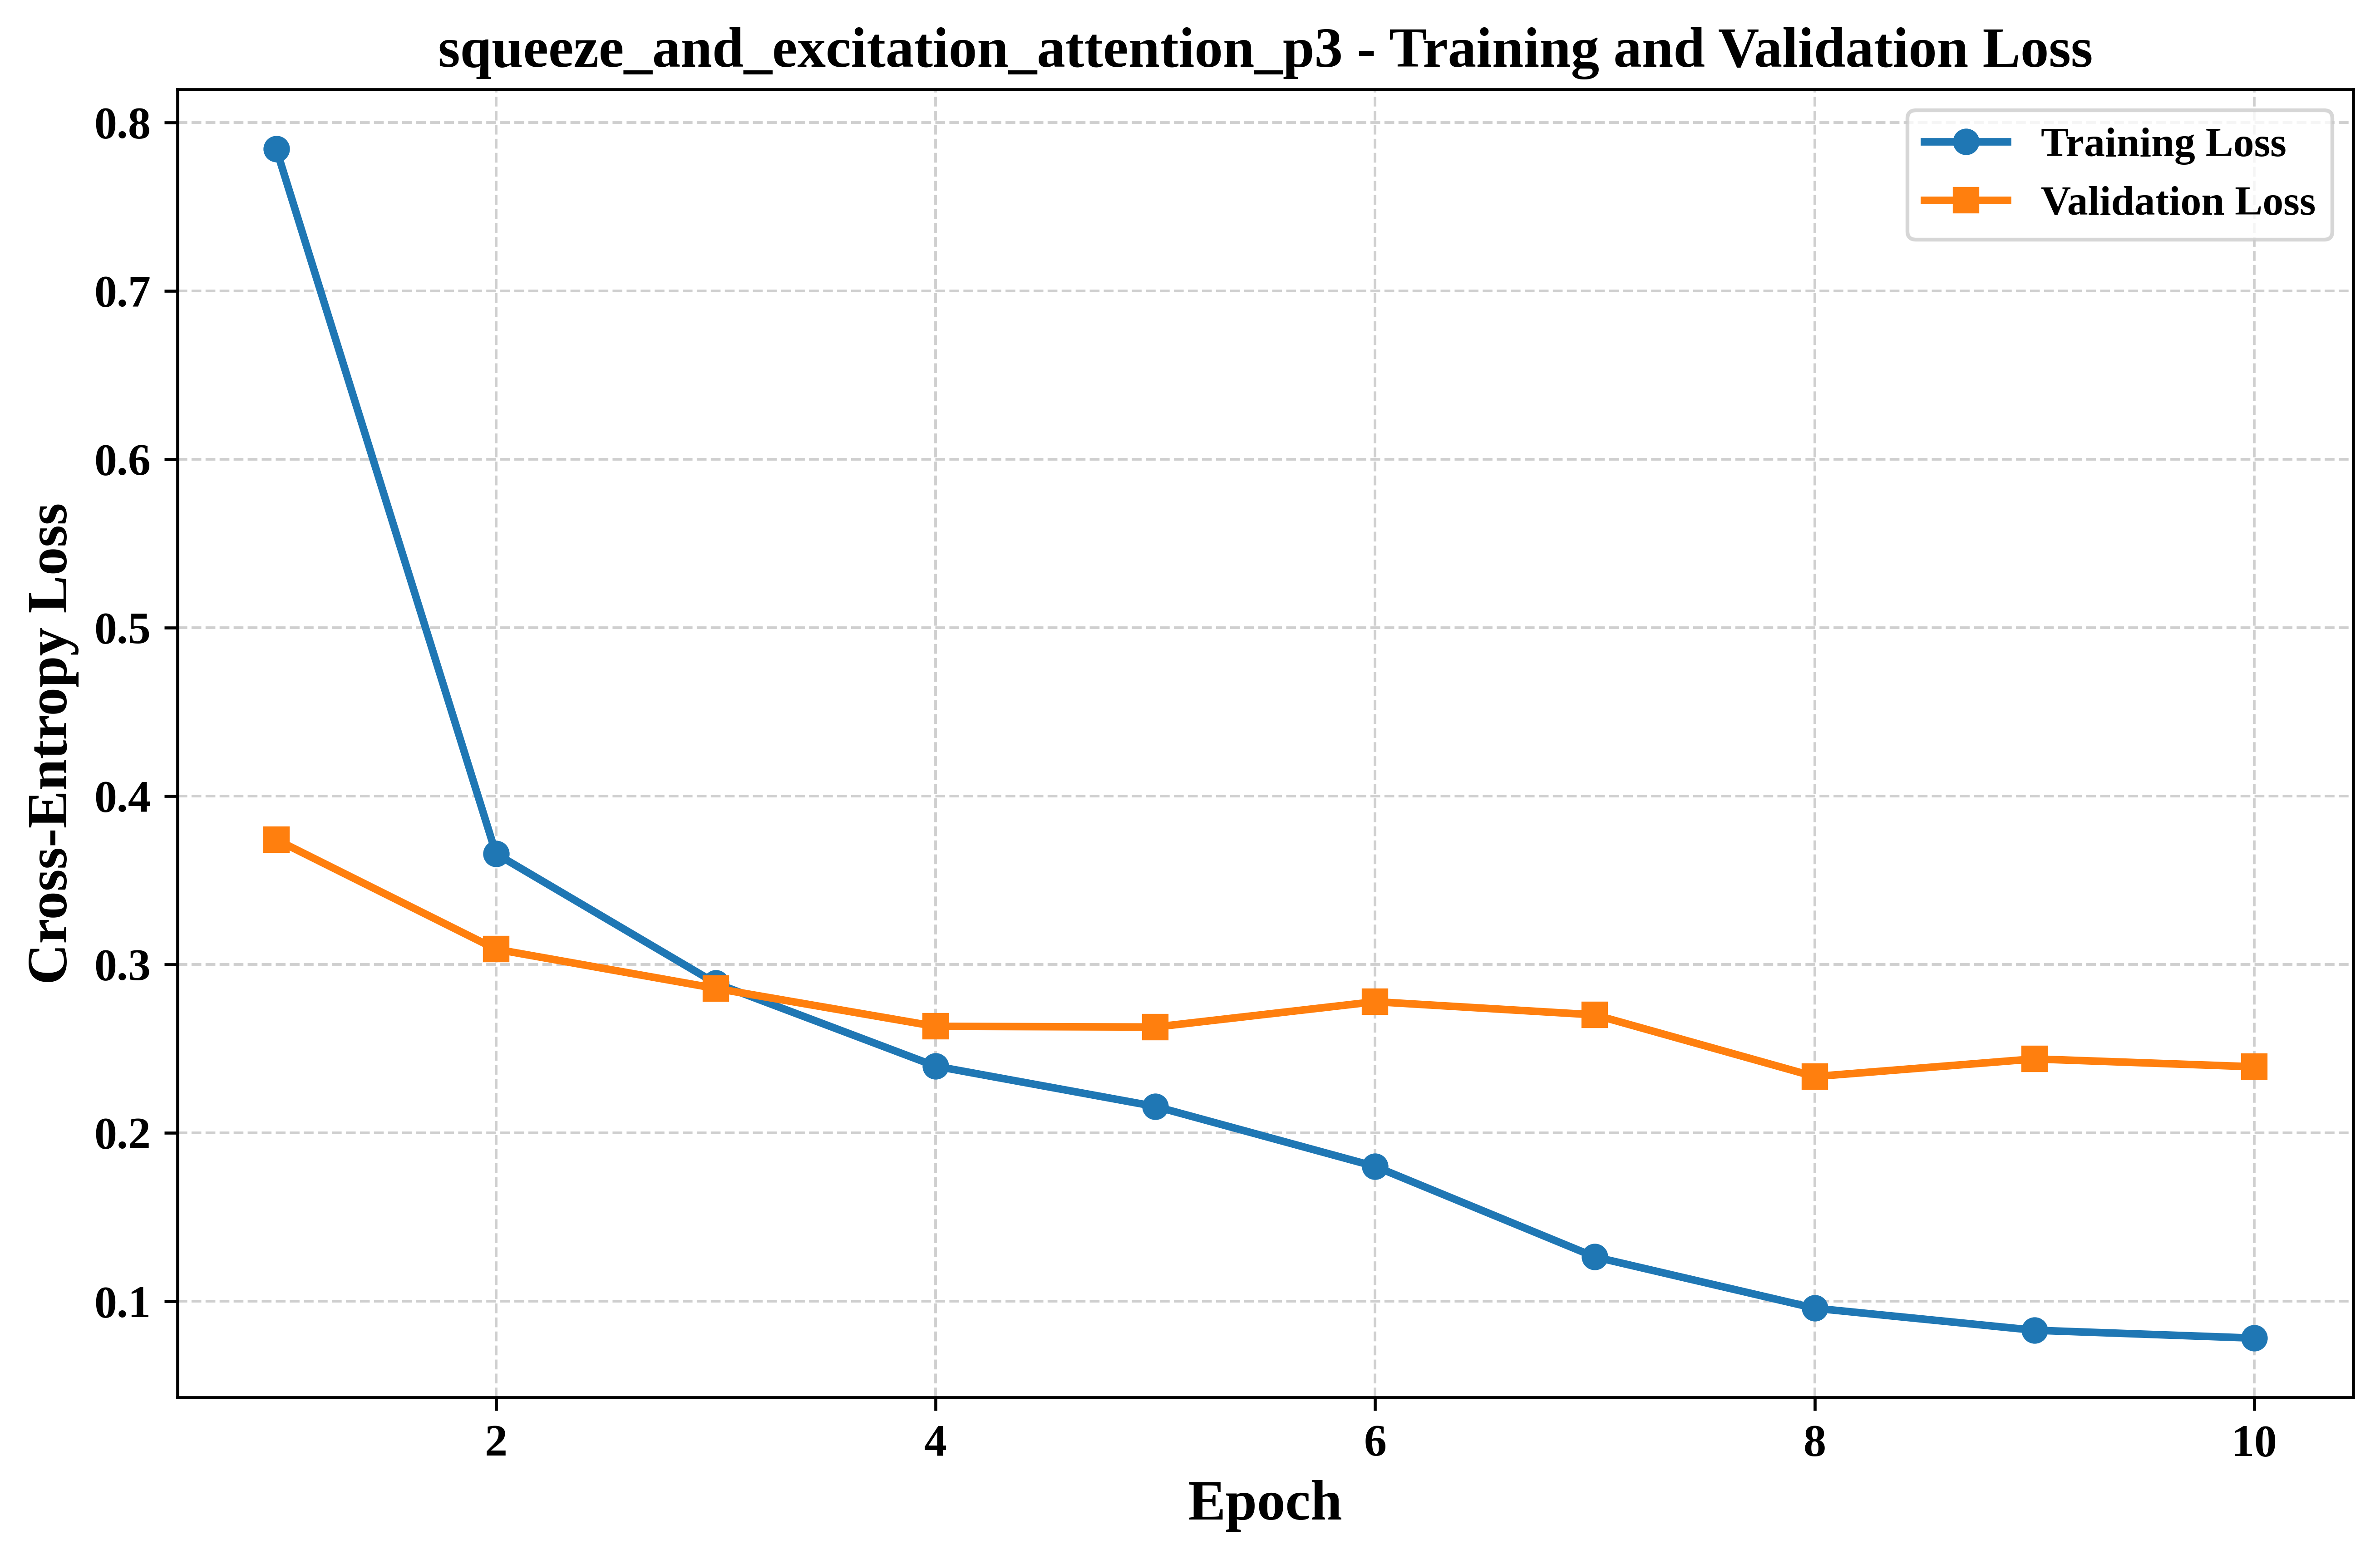
\includegraphics[width=\linewidth]{Images/use/squeeze_and_excitation_attention_p3_loss.png}
    \caption{Training and Validation Loss}
\end{subfigure}

\vspace{2mm}
\begin{subfigure}[b]{0.44\textwidth}
    \centering
    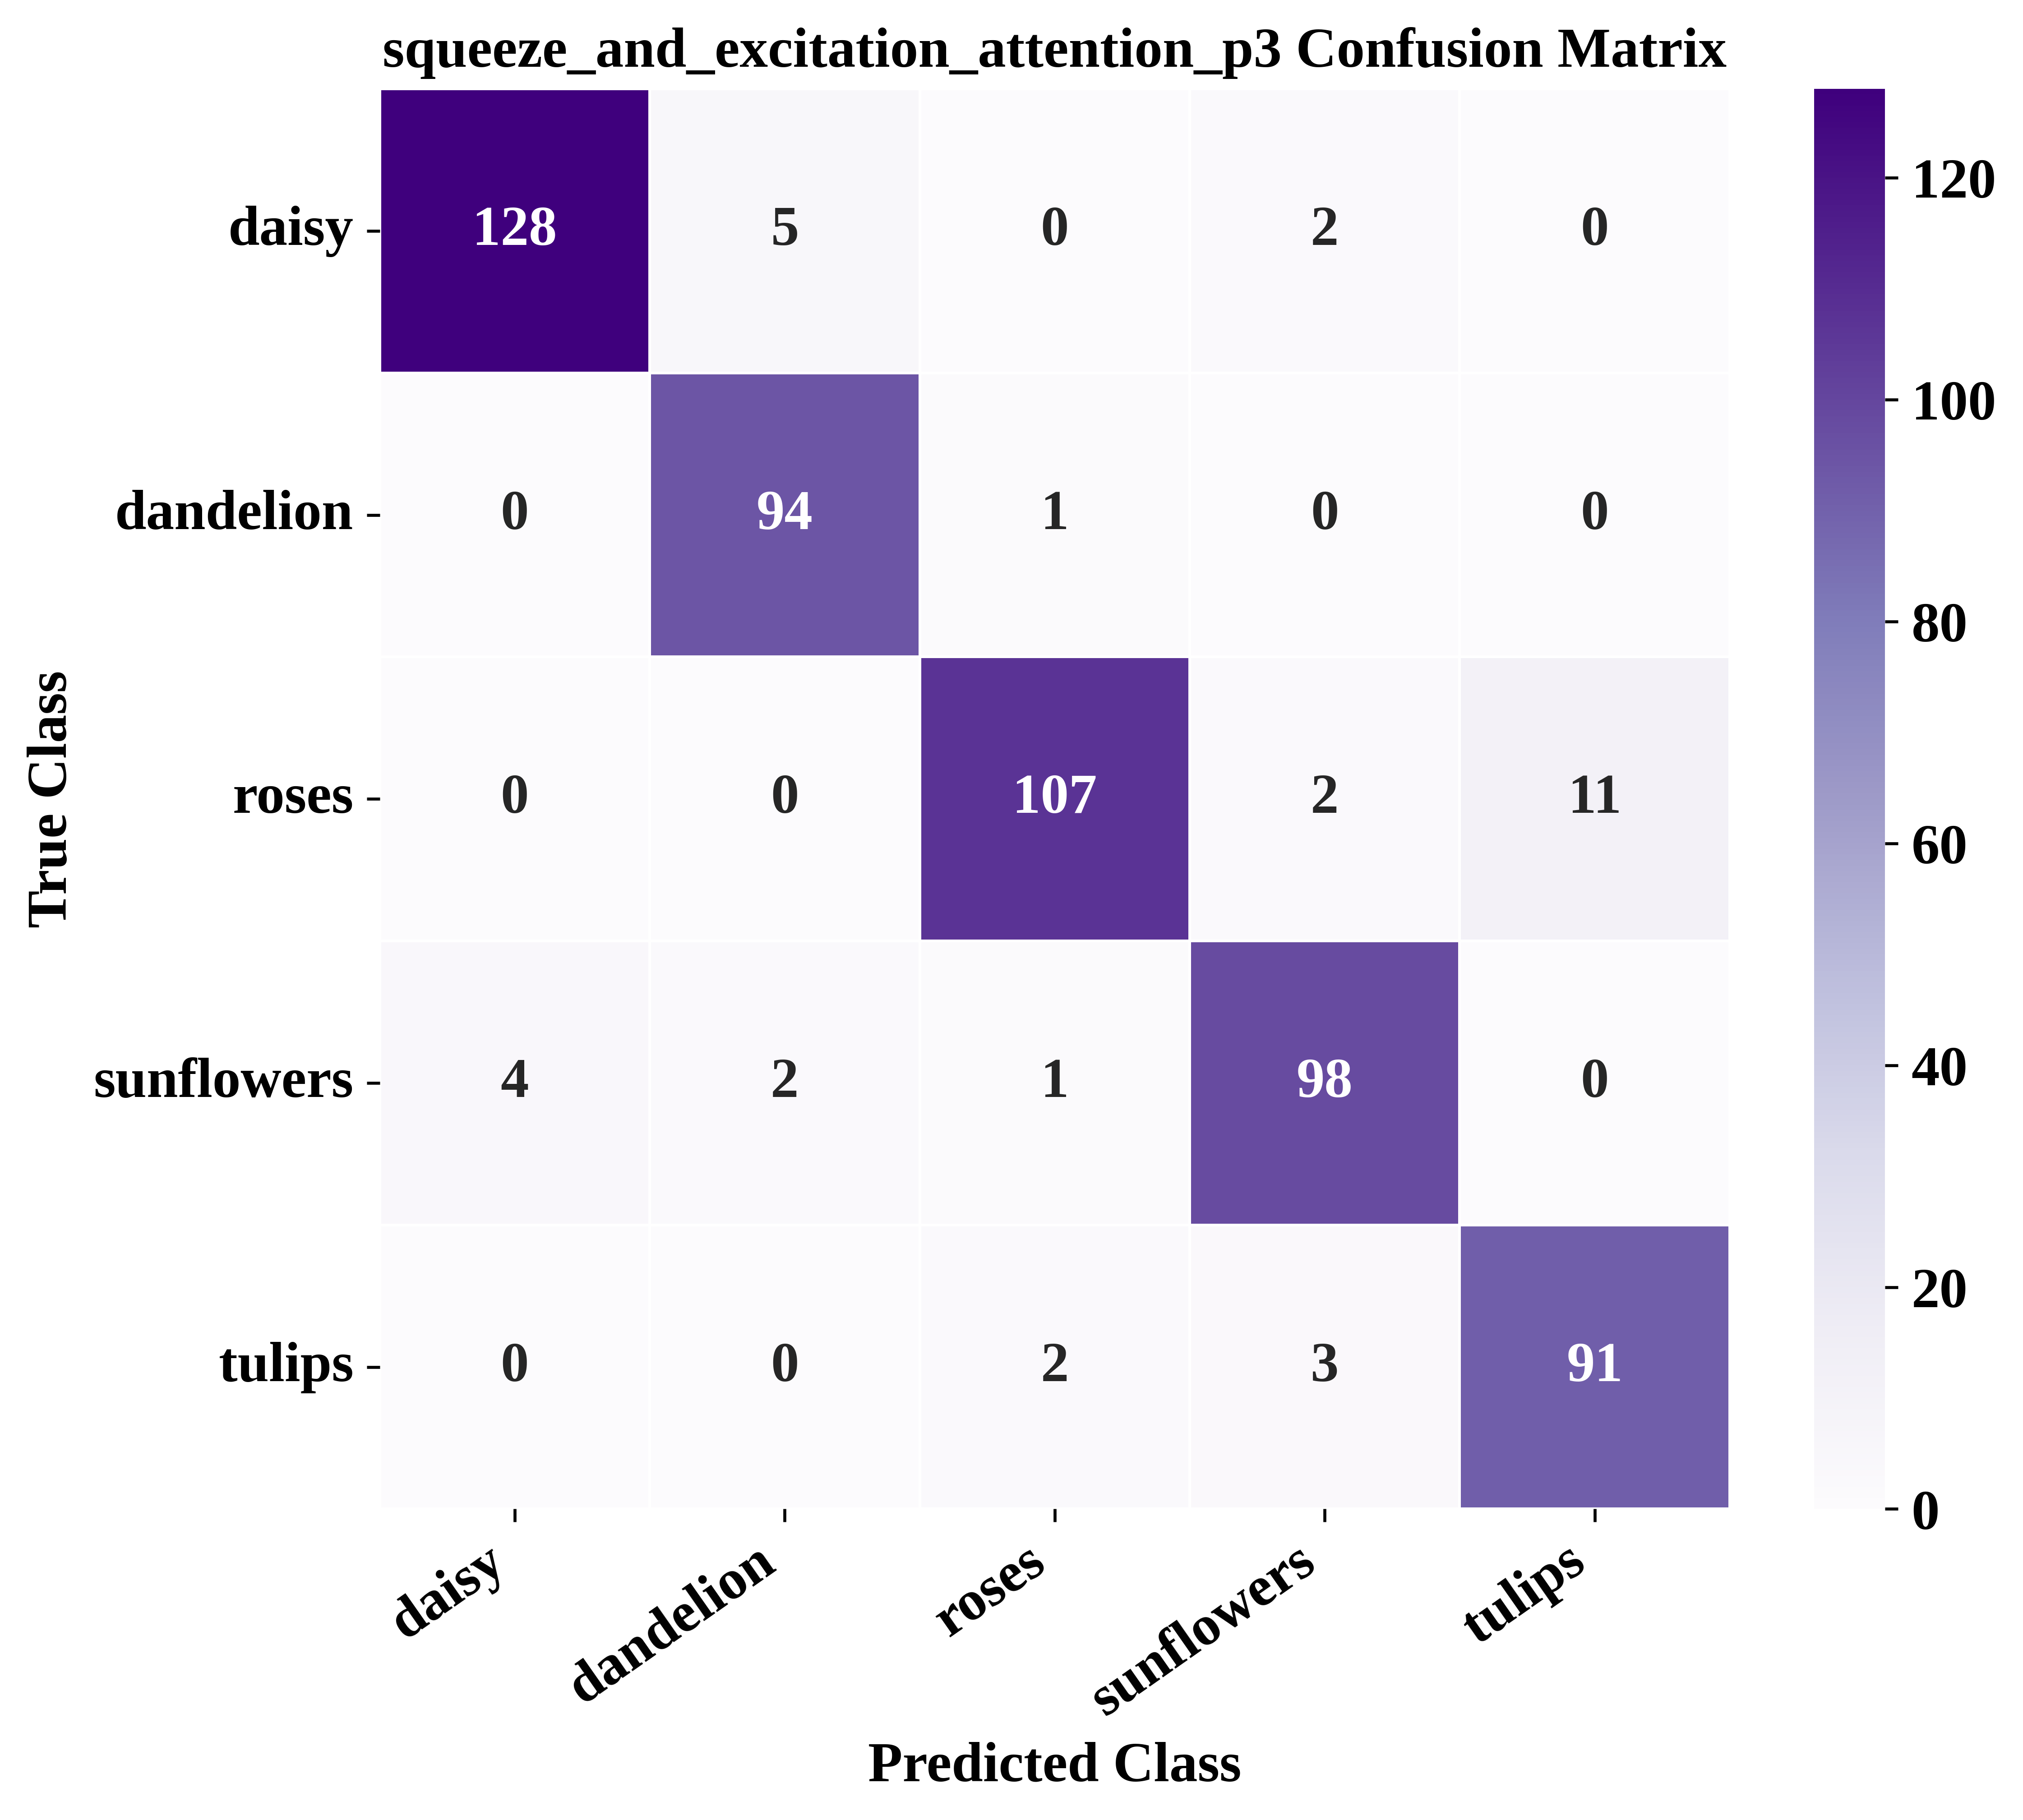
\includegraphics[width=\linewidth]{Images/use/squeeze_and_excitation_attention_p3_confusion_matrix.png}
    \caption{Test Confusion Matrix}
\end{subfigure}
\caption{ResNet50 with Squeeze-and-Excitation (SE) Attention at stage $P_3$: Accuracy trajectories, loss convergence across training epochs, and test confusion matrix.}
\label{fig:se_group}
\end{figure}

\textbf{Inference:} The specialized Squeeze-and-Excitation block at $P_3$ results in good generalization performance with ~92.6\% validation accuracy and loss decay with essentially zero gap between the training and validation curves. Two-stage multi-layer perceptron bottleneck provides non-linear channel dependencies as regularization for the feature representations without any extra parameters overhead. The obtained confusion matrix confirms many true positives on all five classes, showing that channel recalibration results in clear and discriminating feature representations.

\vspace{3mm}

% ------------------------------------------------------------
\subsection*{30.6 Channel+Spatial Attention at $P_2$ (conv2\_x): Accuracy, Loss, and Confusion Matrix}
% ------------------------------------------------------------

\begin{figure}[H]
\centering
\begin{subfigure}[b]{0.485\textwidth}
    \centering
    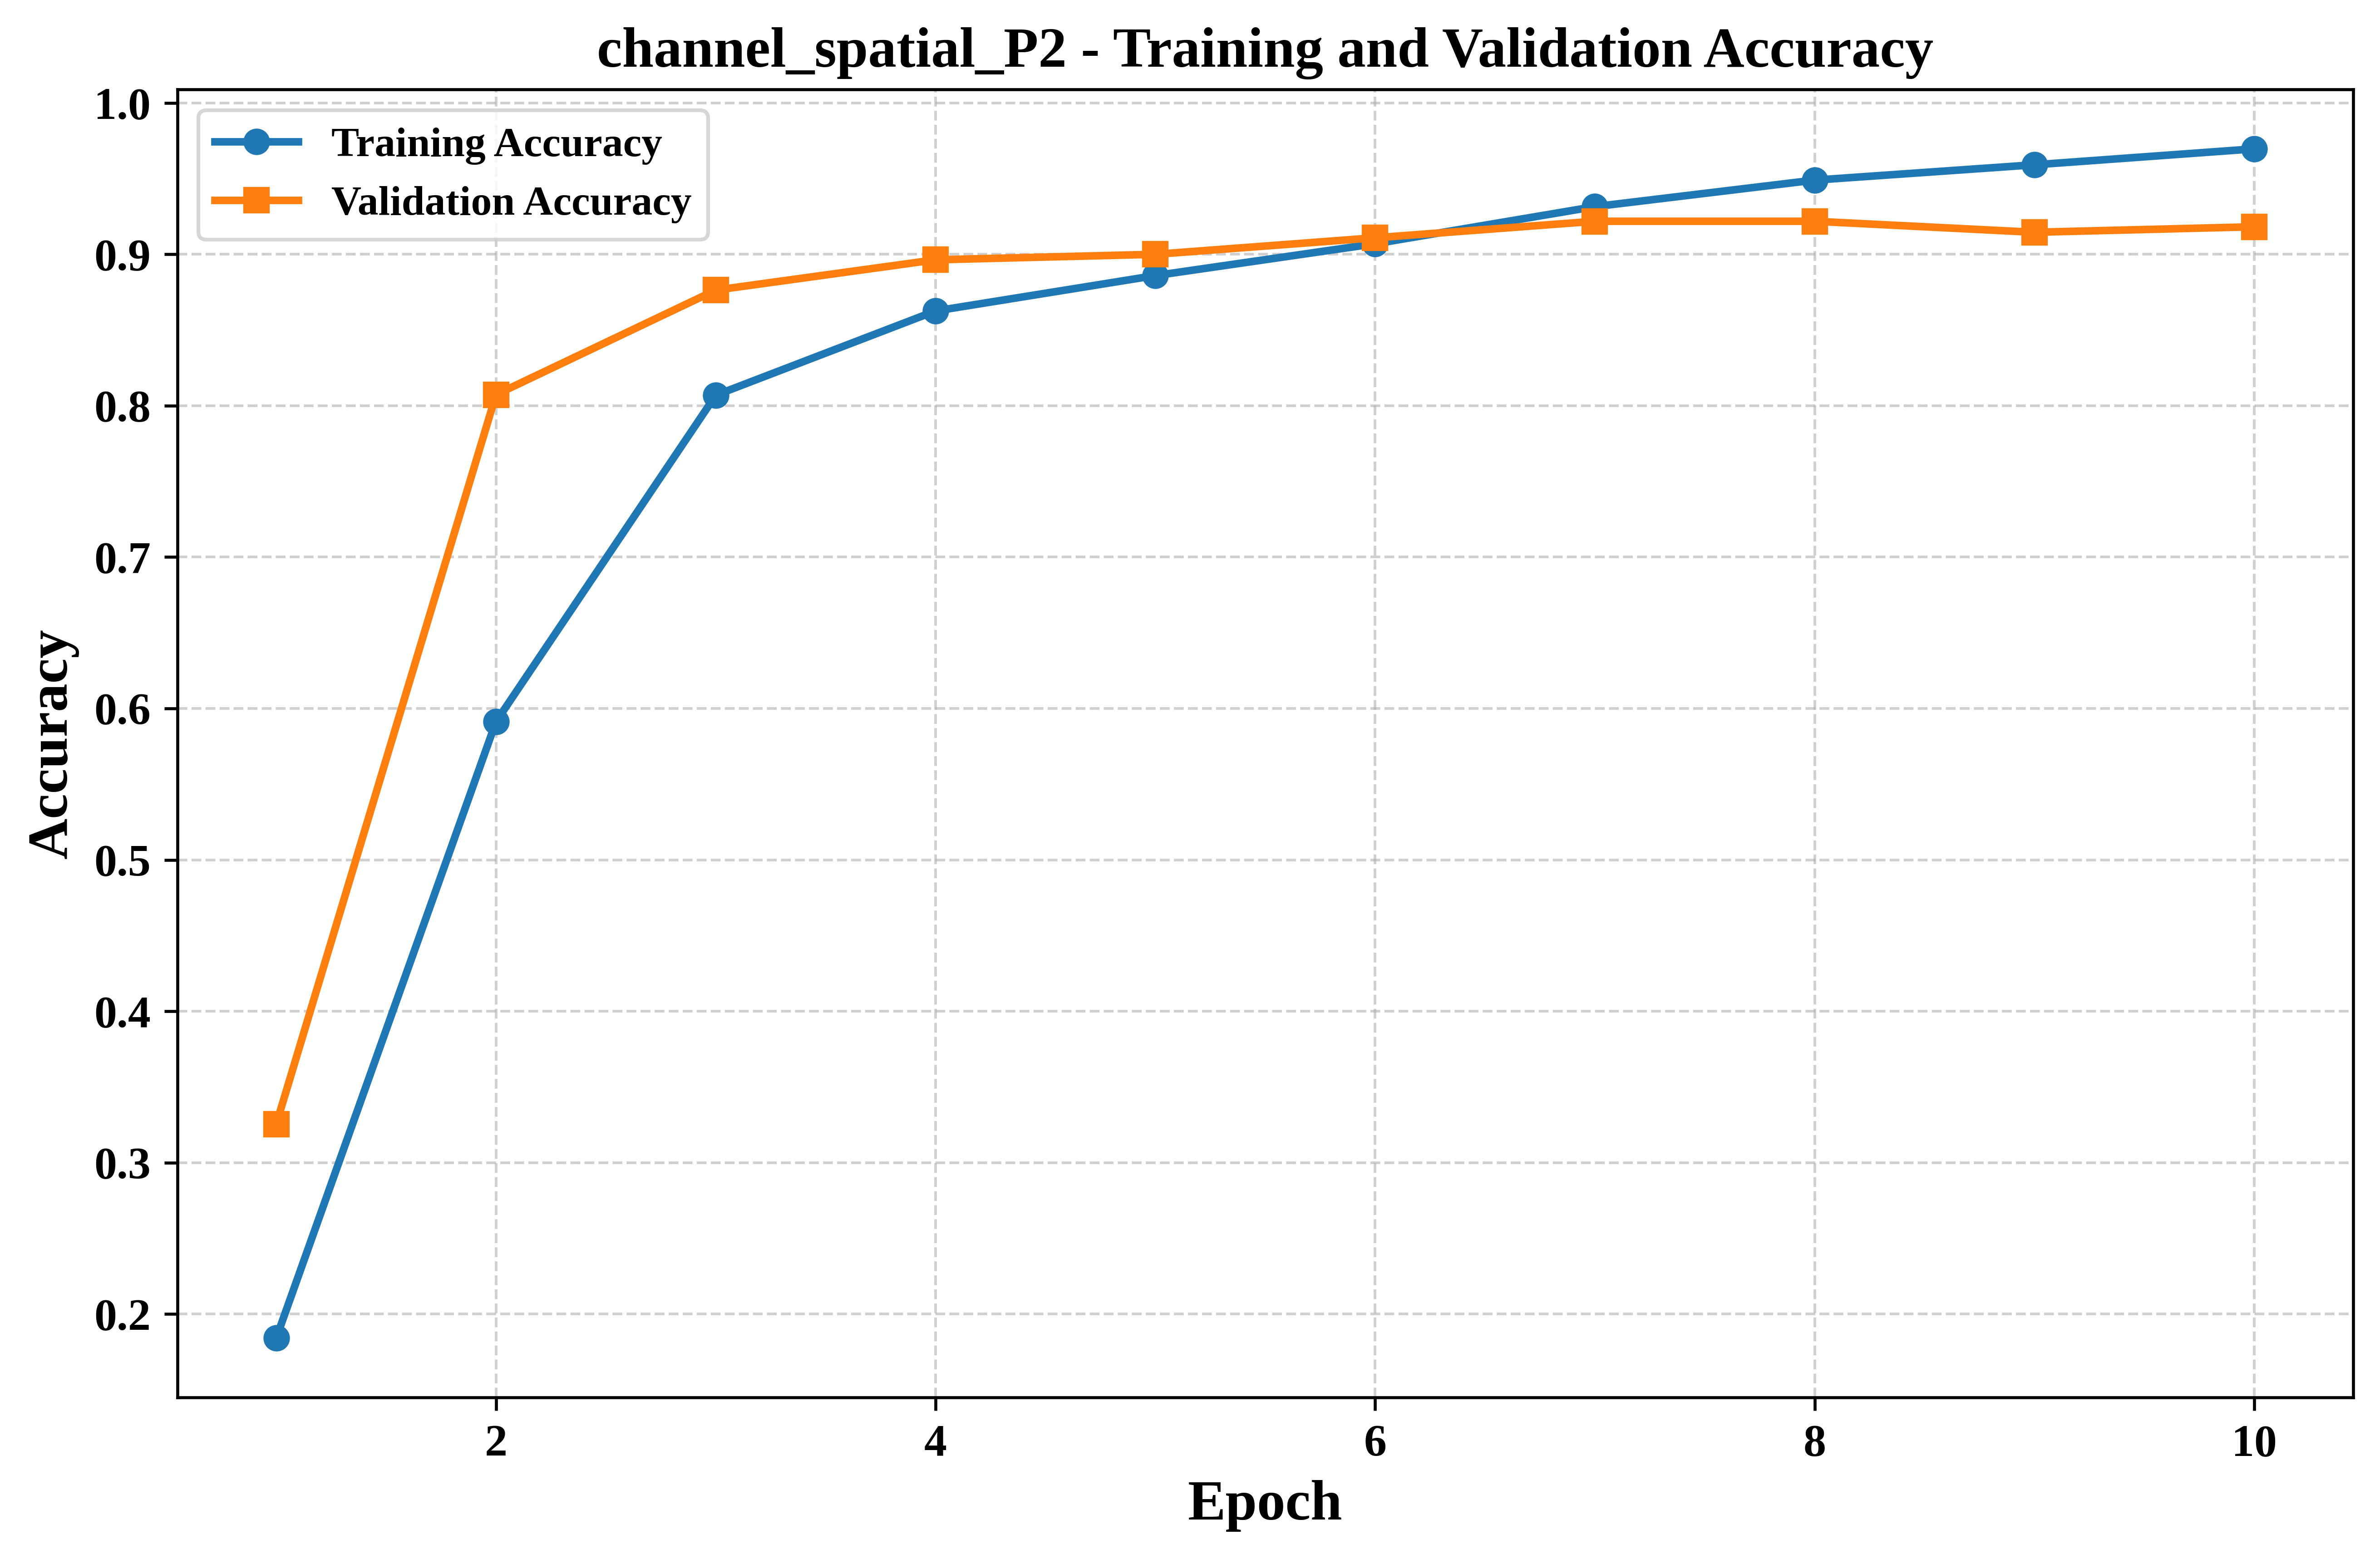
\includegraphics[width=\linewidth]{Images/use/channel_spatial_P2_accuracy.png}
    \caption{Training and Validation Accuracy}
\end{subfigure}
\hfill
\begin{subfigure}[b]{0.485\textwidth}
    \centering
    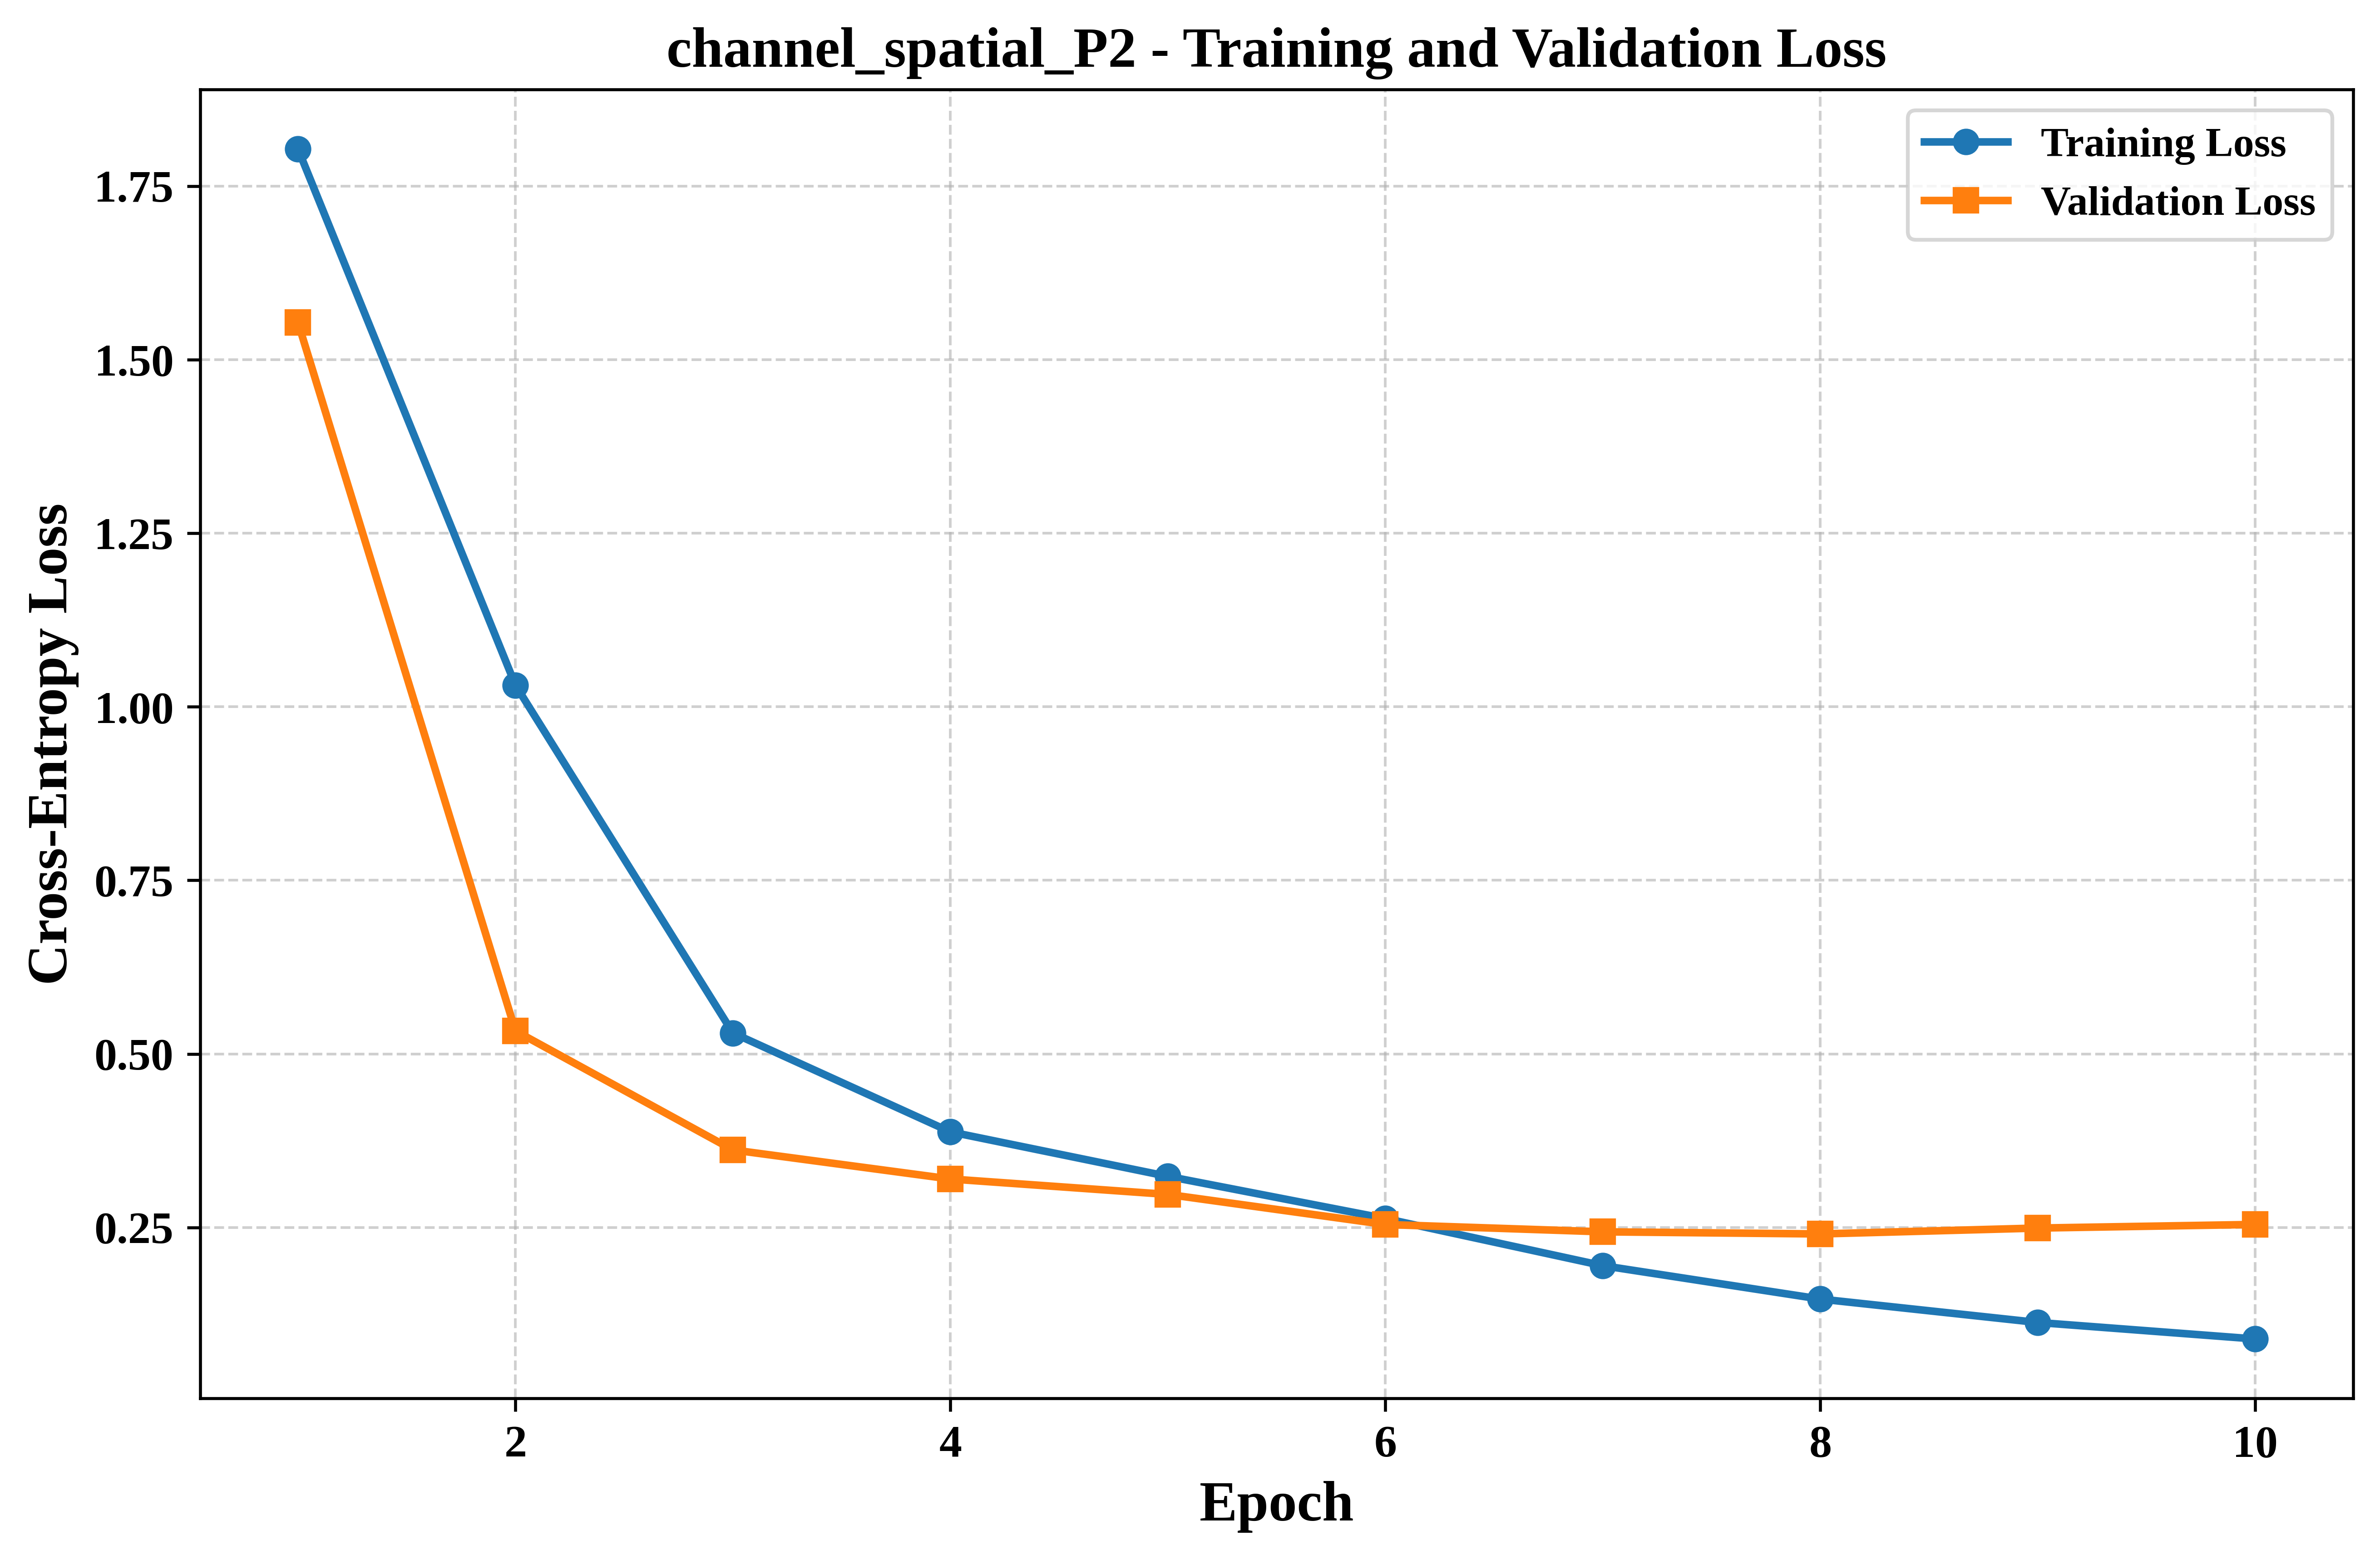
\includegraphics[width=\linewidth]{Images/use/channel_spatial_P2_loss.png}
    \caption{Training and Validation Loss}
\end{subfigure}

\vspace{2mm}
\begin{subfigure}[b]{0.44\textwidth}
    \centering
    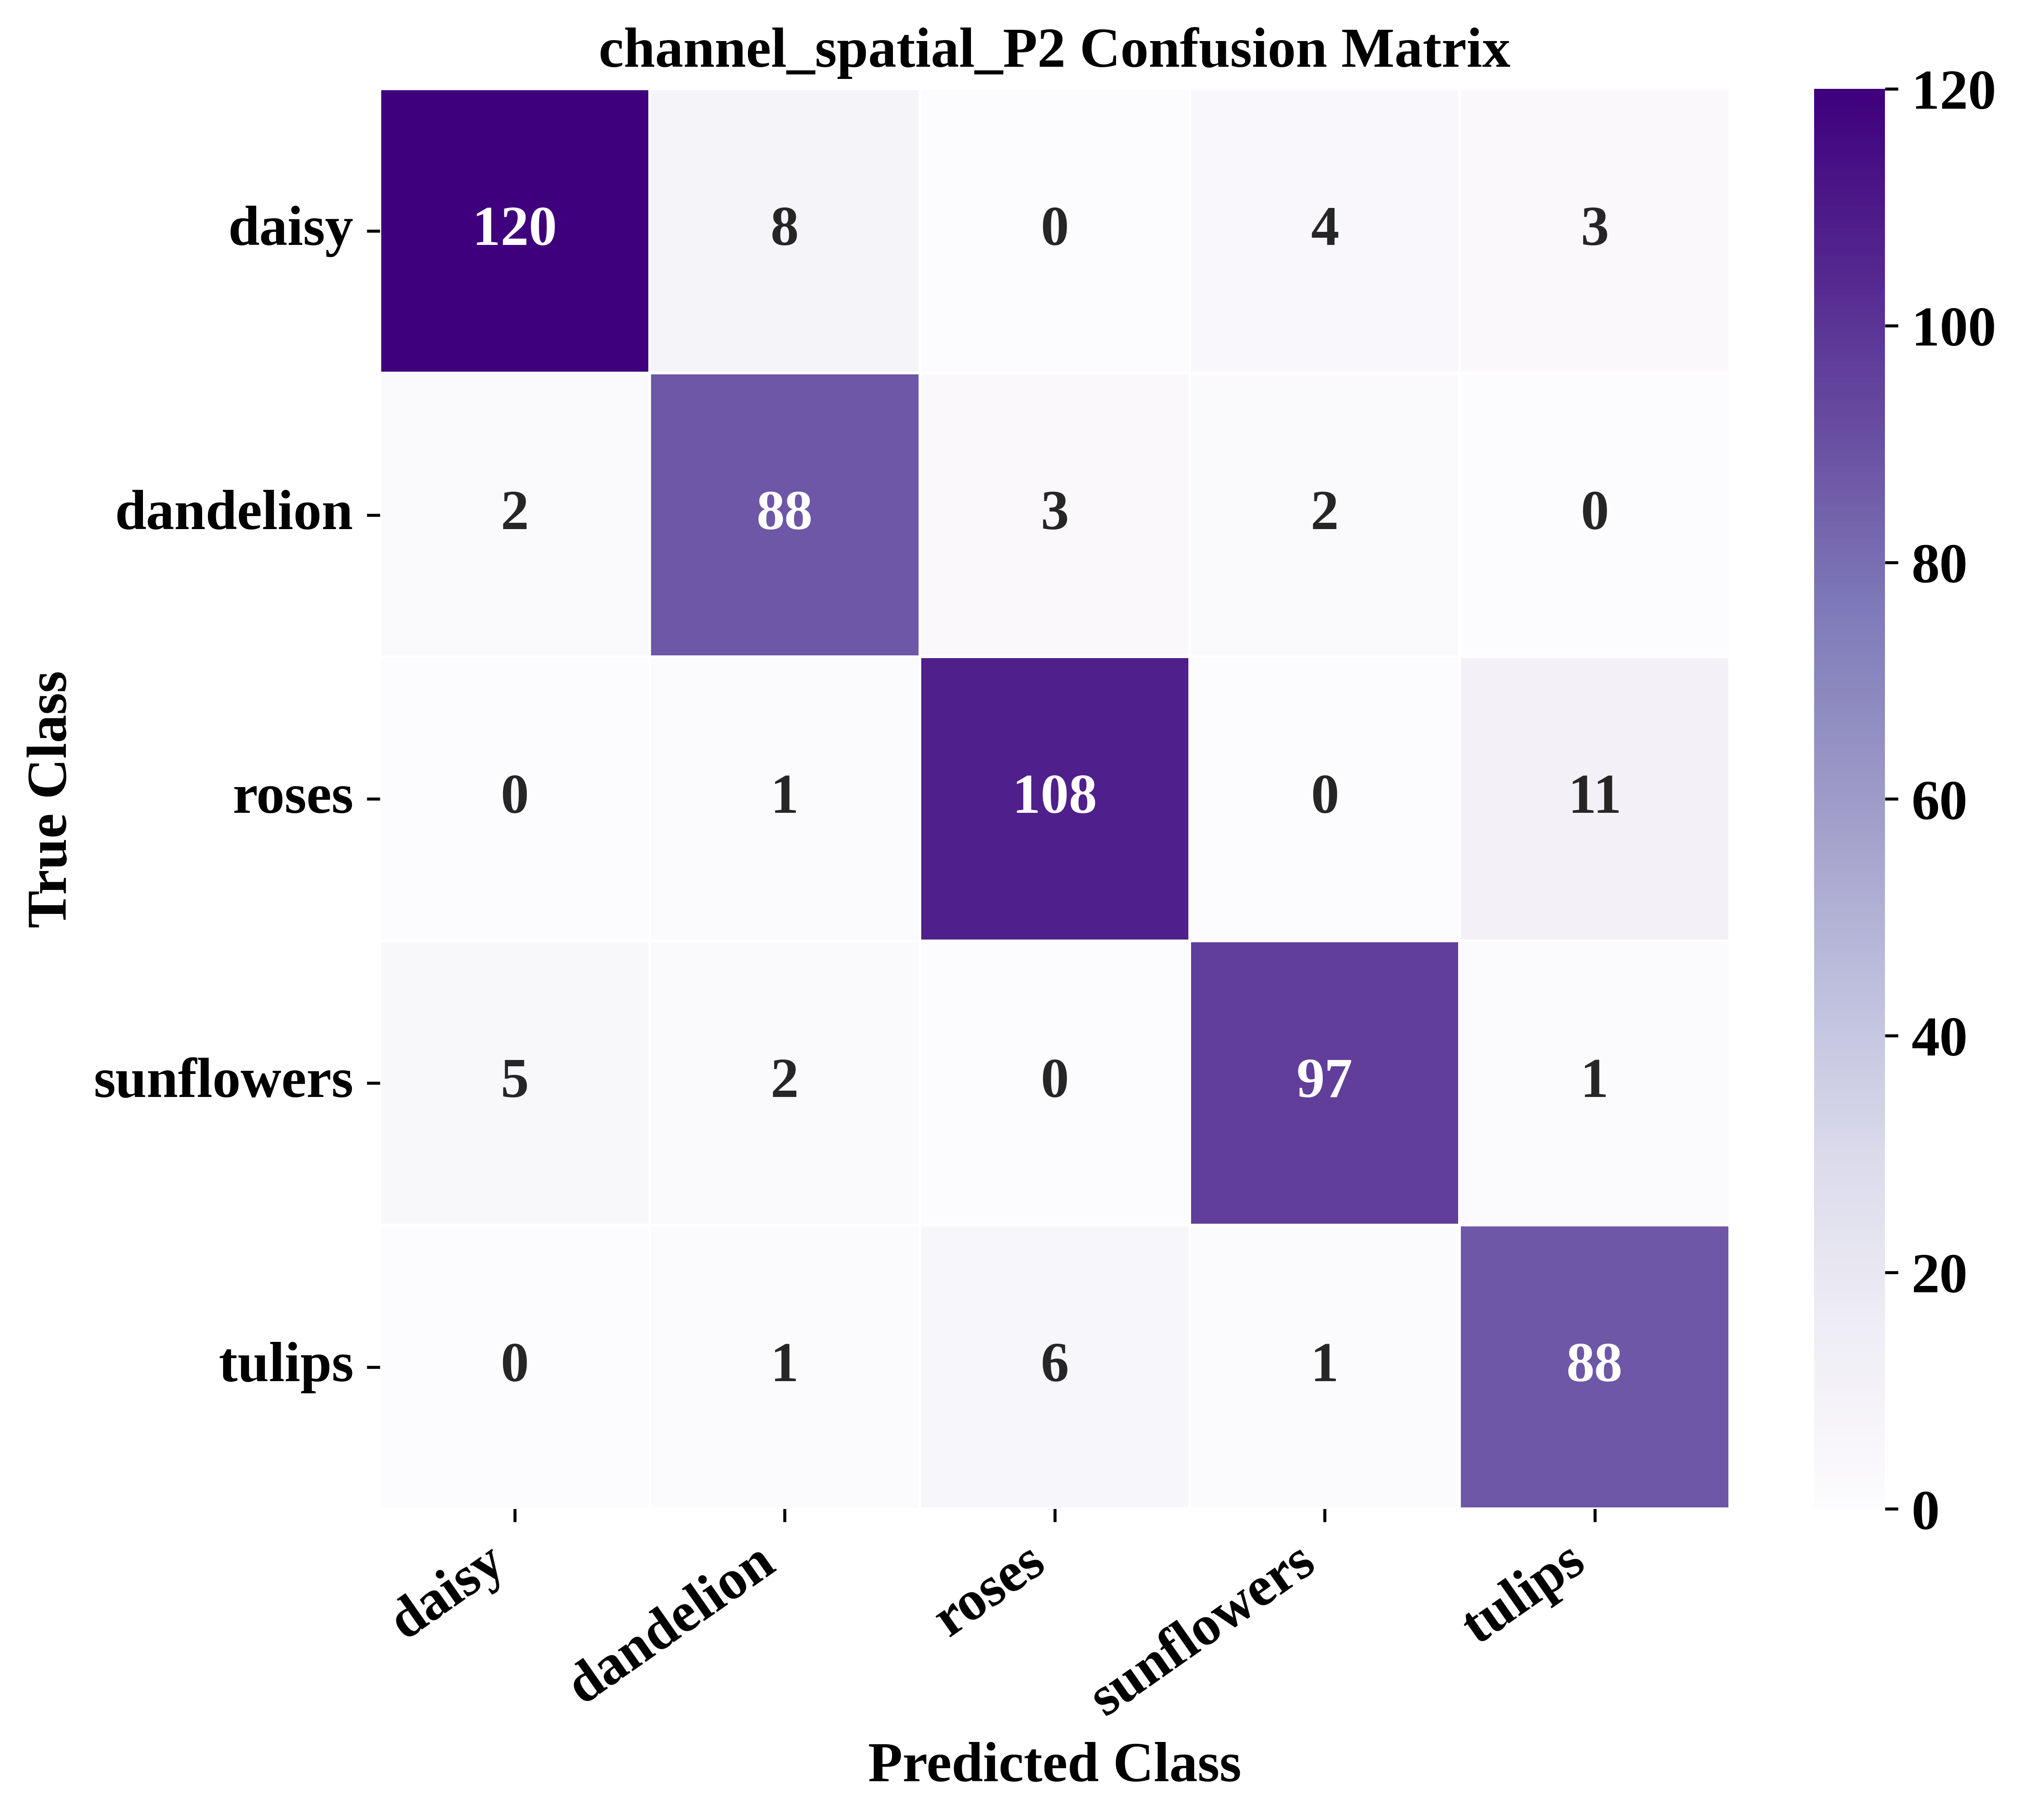
\includegraphics[width=\linewidth]{Images/use/channel_spatial_P2_confusion_matrix.png}
    \caption{Test Confusion Matrix}
\end{subfigure}
\caption{ResNet50 with Sequential Channel+Spatial Attention at early stage $P_2$ (conv2\_x): Training and validation accuracy curves, loss descent, and test confusion matrix.}
\label{fig:cs_p2_group}
\end{figure}

\textbf{Inference:} Adding of sequential Channel+Spatial attention at an early stage of $P_2$ provides good control of low-level feature refinement, achieving 91.2\% test accuracy and smooth convergence of the loss curve. However, due to the high spatial resolution of features at $P_2$ ($56 \times 56$) with simple edge/texture semantics, the attention blocks do not have enough of high-level semantics to utilize their full potential. From the confusion matrix it can be seen that there is relatively good separation of the classes, however class confusion is somewhat higher compared to intermediate stage $P_3$.

\vspace{3mm}

% ------------------------------------------------------------
\subsection*{30.7 Multi-Stage Channel+Spatial Attention ($P_2+P_3+P_4$): Accuracy, Loss, and Confusion Matrix}
% ------------------------------------------------------------

\begin{figure}[H]
\centering
\begin{subfigure}[b]{0.485\textwidth}
    \centering
    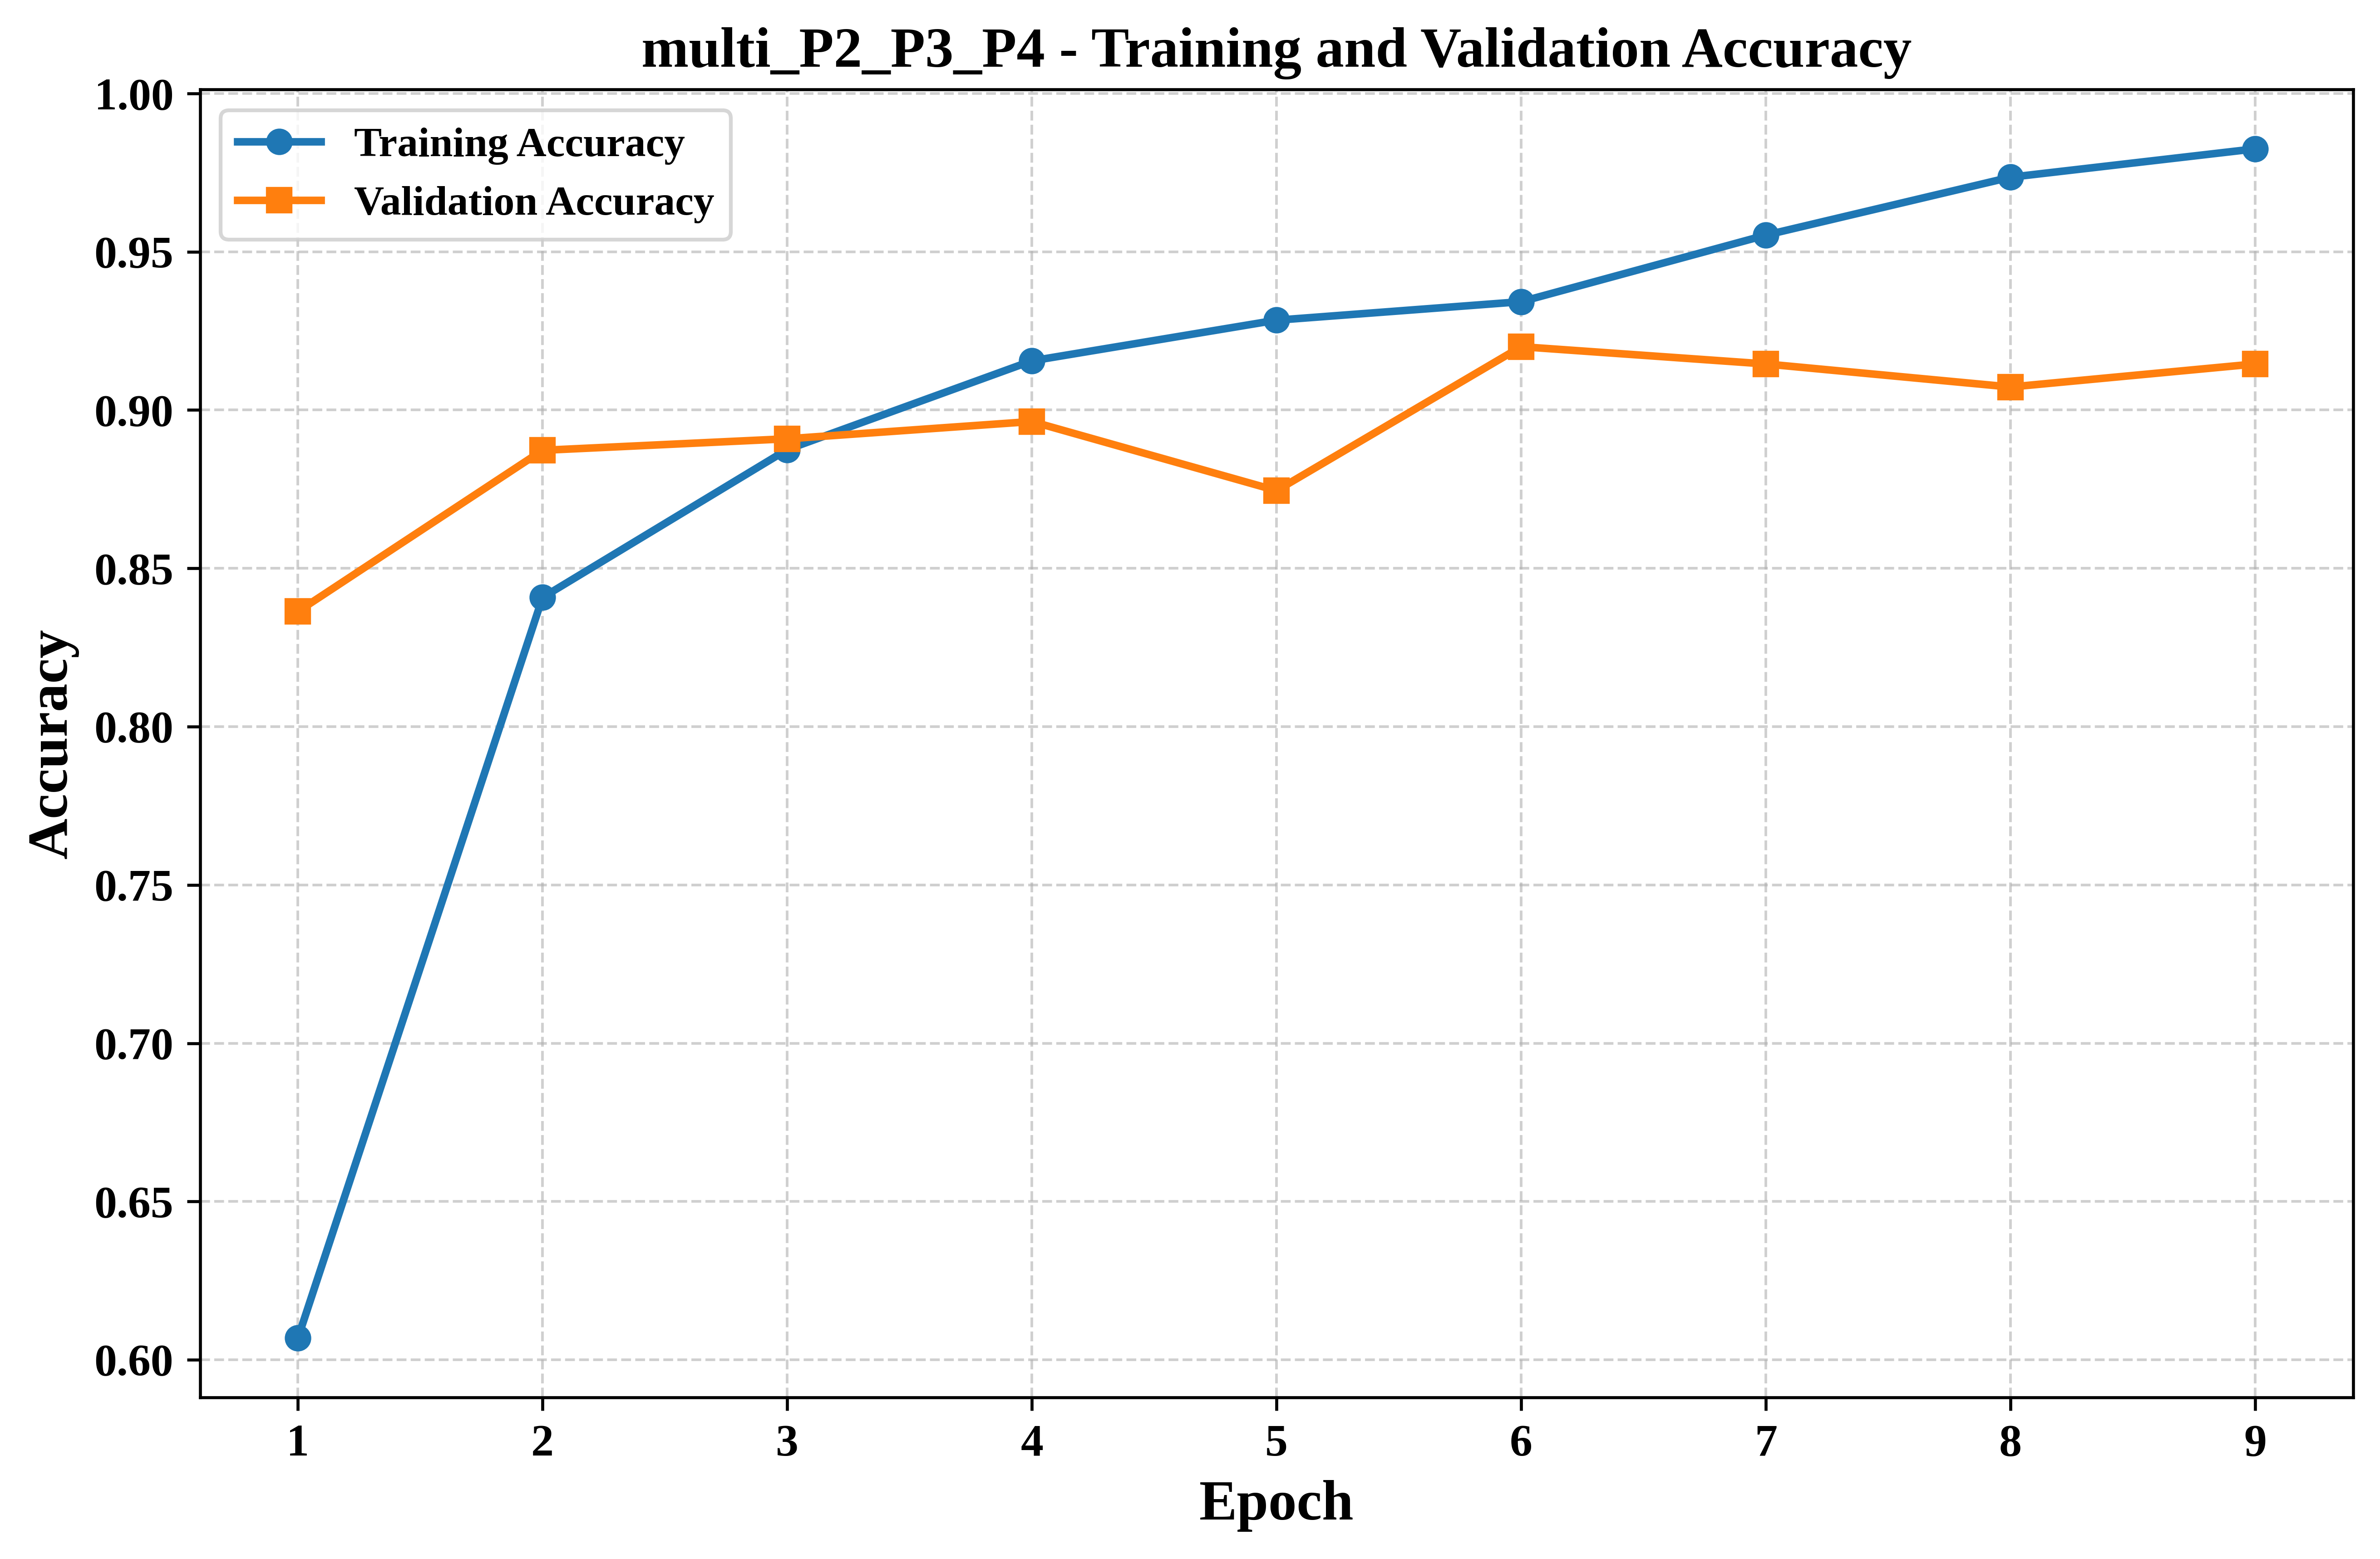
\includegraphics[width=\linewidth]{Images/use/multi_P2_P3_P4_accuracy.png}
    \caption{Training and Validation Accuracy}
\end{subfigure}
\hfill
\begin{subfigure}[b]{0.485\textwidth}
    \centering
    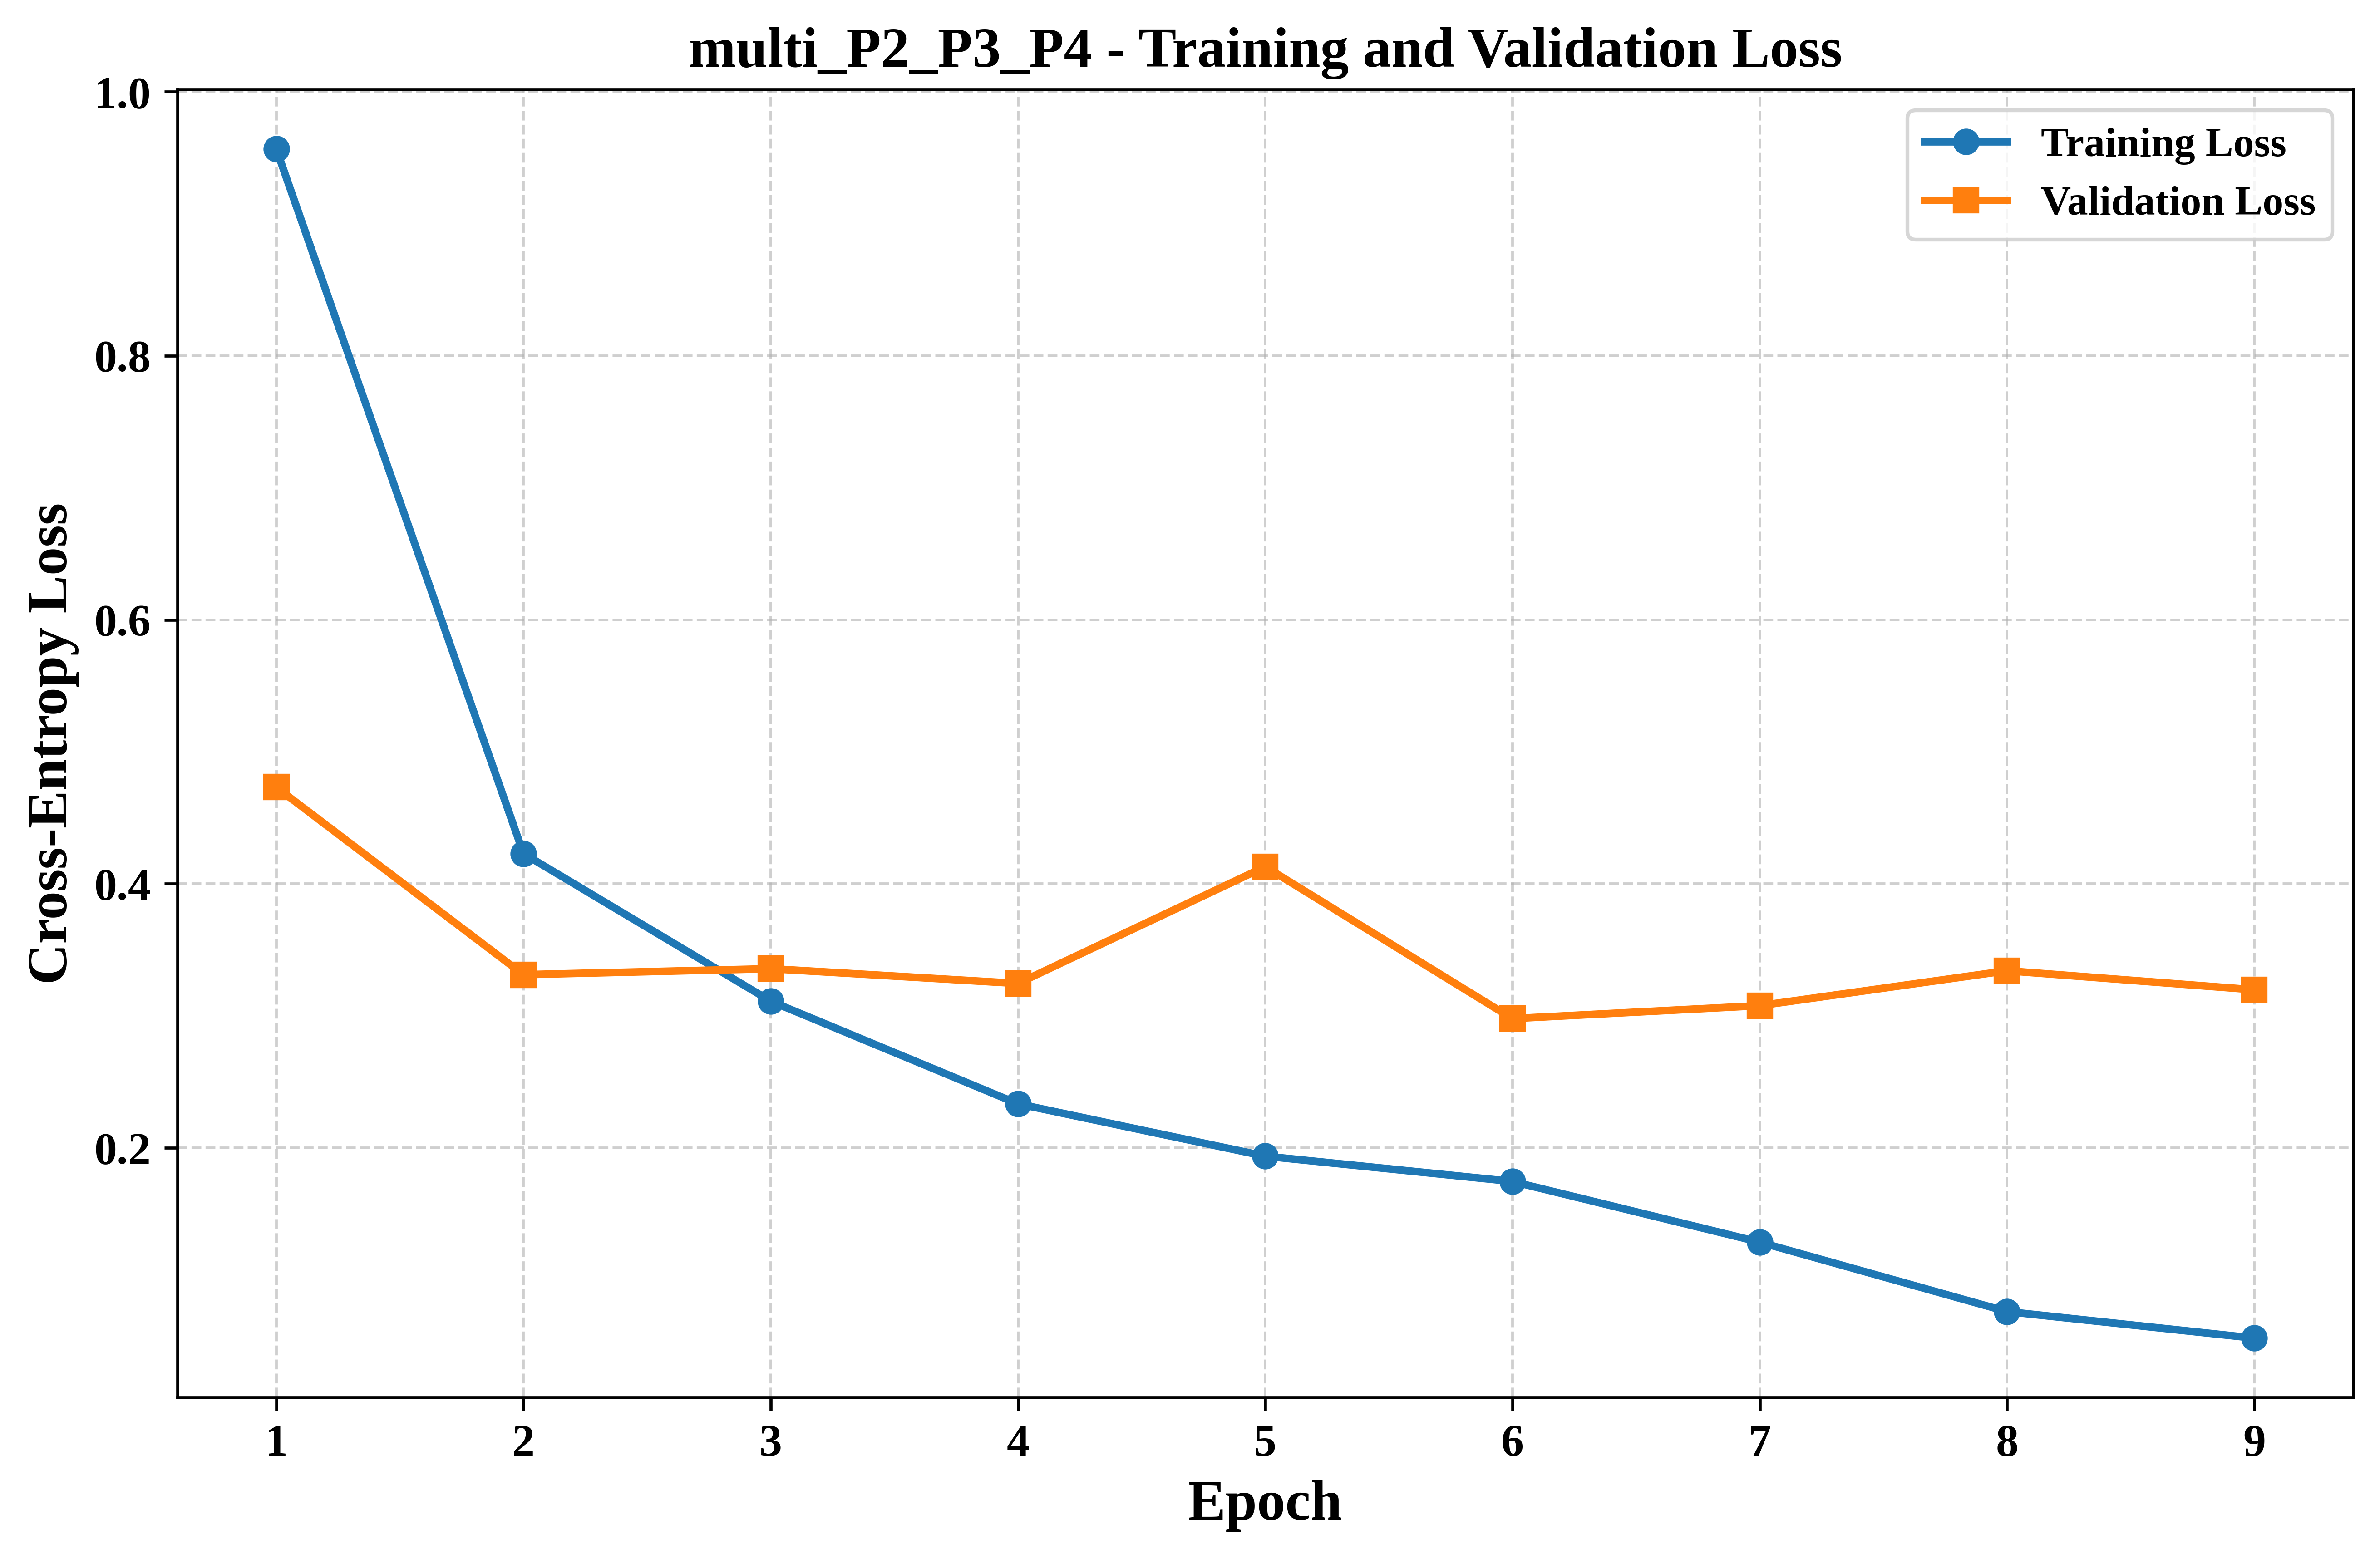
\includegraphics[width=\linewidth]{Images/use/multi_P2_P3_P4_loss.png}
    \caption{Training and Validation Loss}
\end{subfigure}

\vspace{2mm}
\begin{subfigure}[b]{0.44\textwidth}
    \centering
    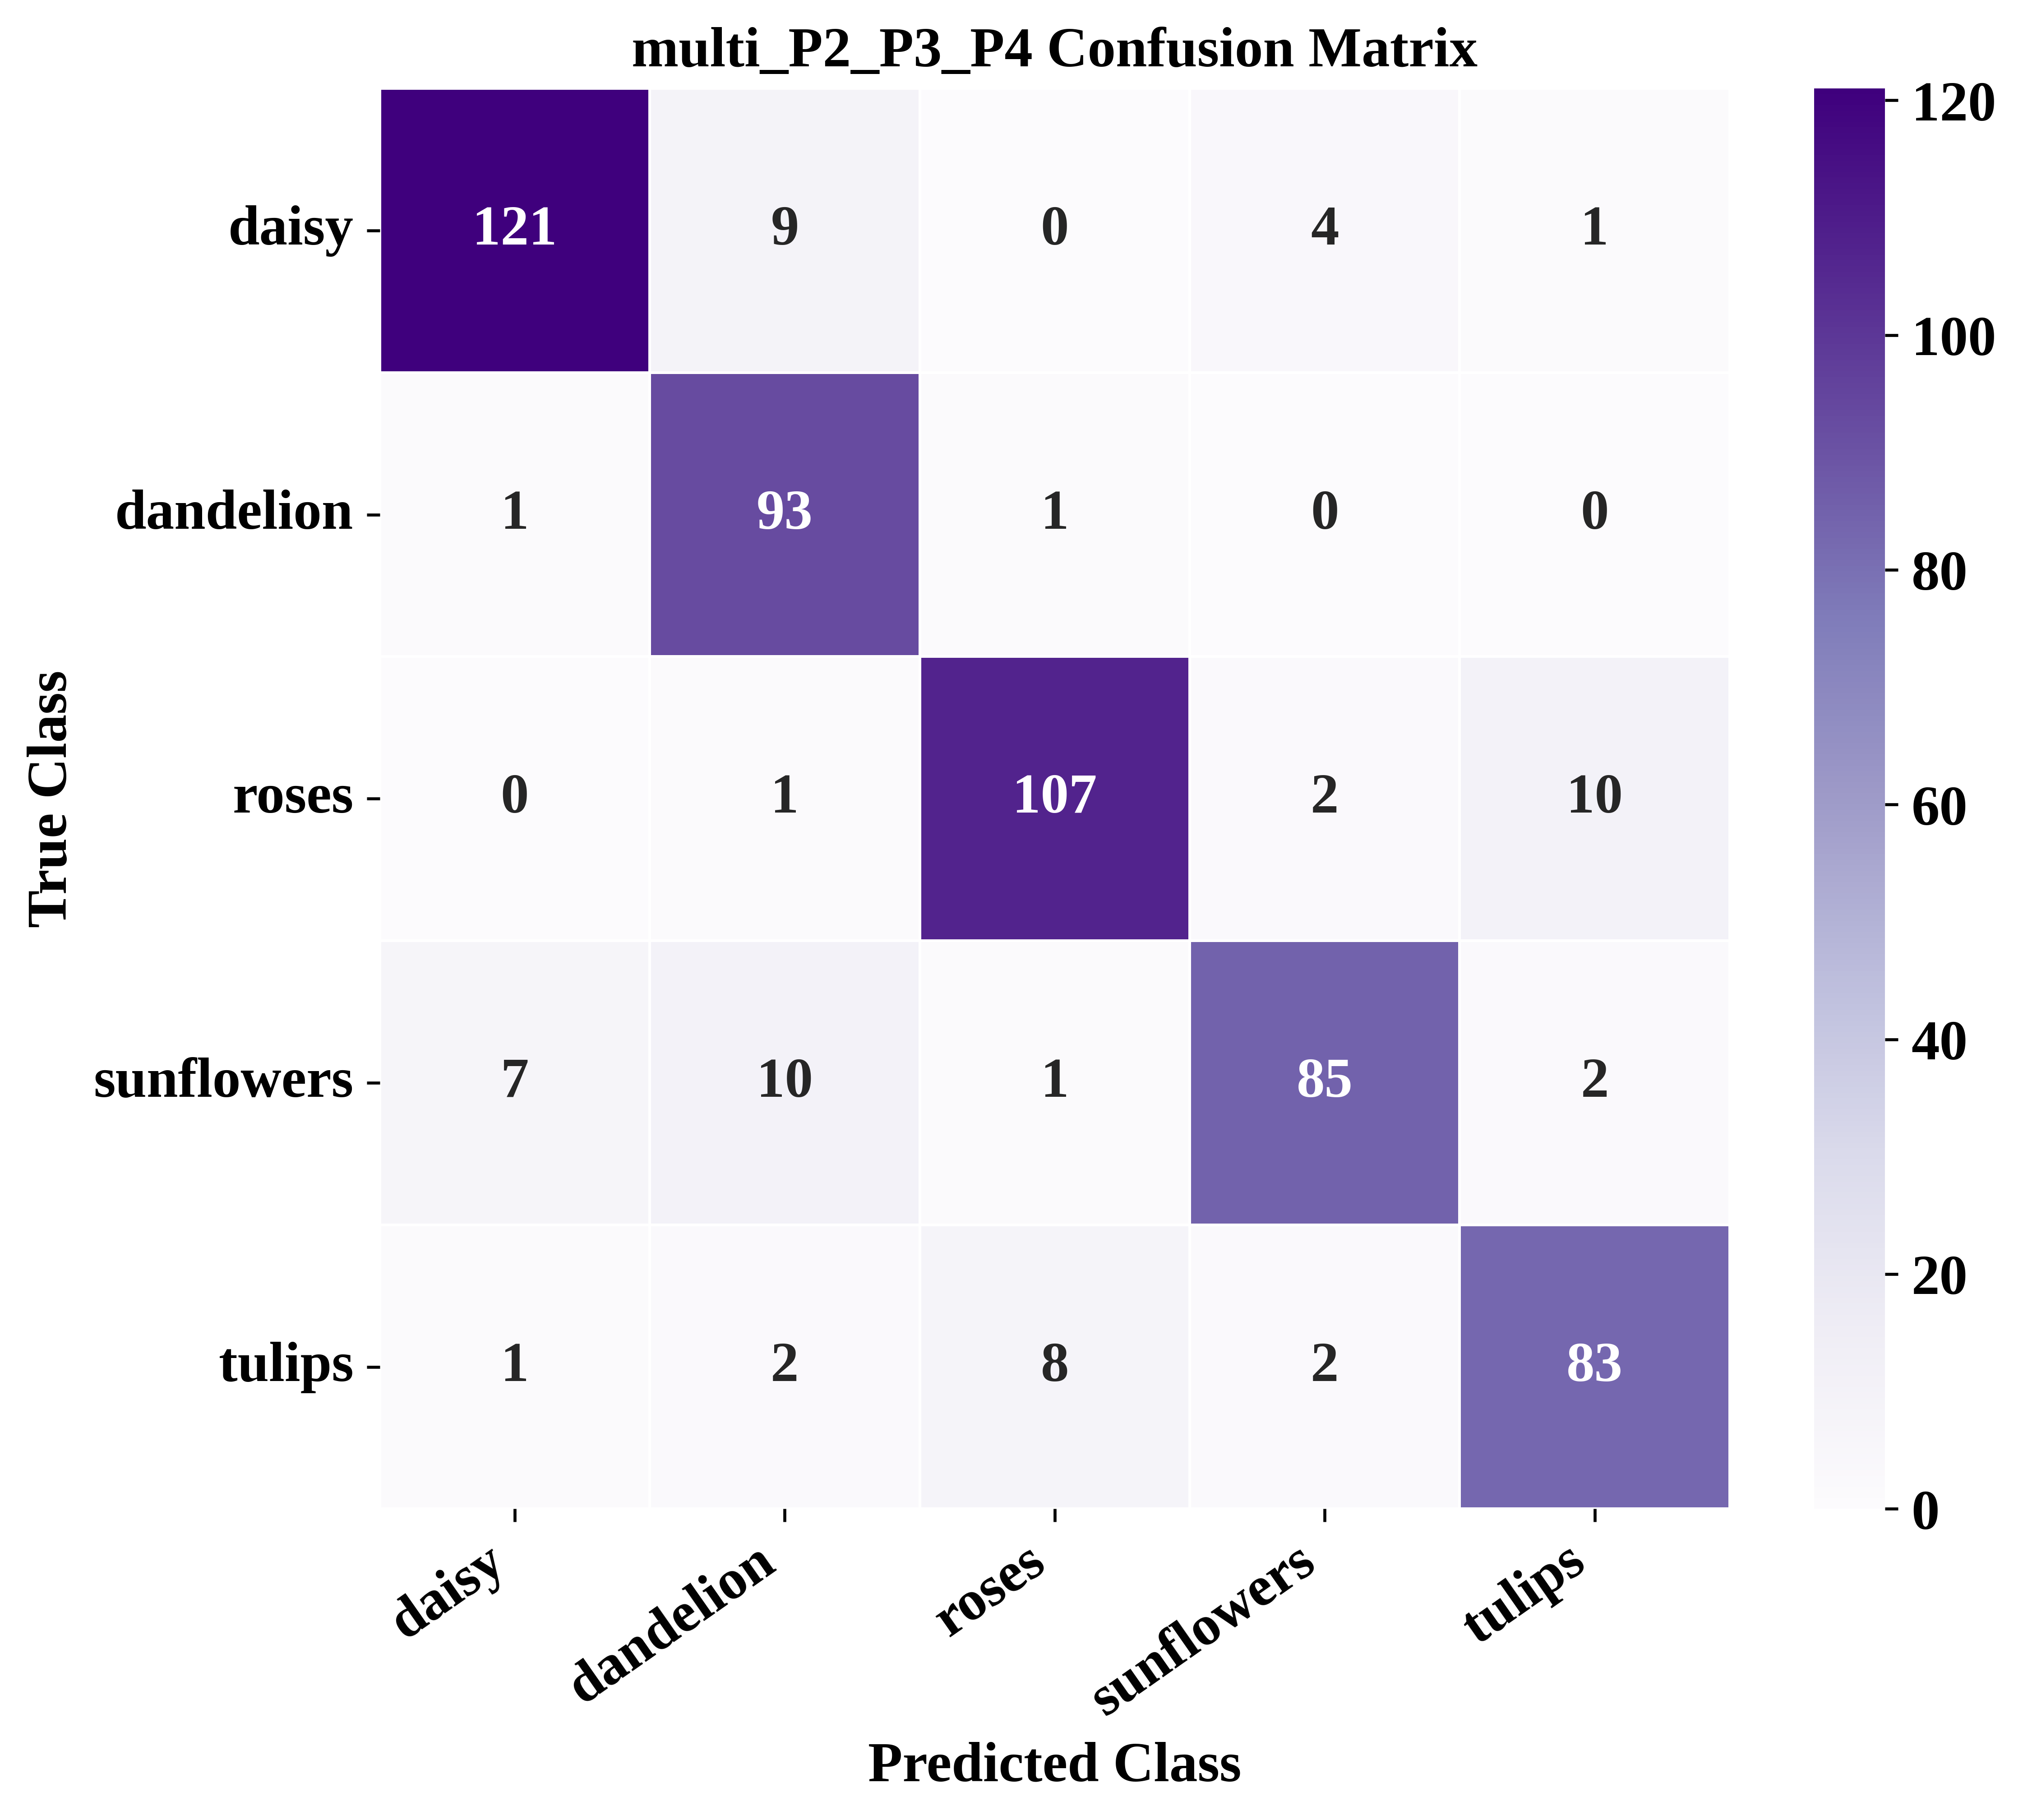
\includegraphics[width=\linewidth]{Images/use/multi_P2_P3_P4_confusion_matrix.png}
    \caption{Test Confusion Matrix}
\end{subfigure}
\caption{ResNet50 with Multi-Stage Attention applied simultaneously across stages $P_2$, $P_3$, and $P_4$: Accuracy and loss profiles alongside test confusion matrix.}
\label{fig:multi_p234_group}
\end{figure}

\textbf{Inference:} Inserting attention blocks during stages $P_2$, $P_3$, and $P_4$ at once leads to slightly worse test accuracy (88.9\%) and, in contrast to single-stage attention insertion at stage $P_3$, this approach demonstrates much lower results (92.4\%). Based on loss curves, one can notice early validation plateauing; hence, cascade insertion of attention modules increases parameter number and, consequently, makes a network more vulnerable to overfitting on a moderate-size training set. Confusion matrix demonstrates higher off-diagonal errors' dispersion that proves empirically the superiority of targeted attention insertion at a single important stage.

\vspace{3mm}

% ------------------------------------------------------------
\subsection*{30.8 Comparative Confusion Matrix Analysis: Baseline vs. Channel$\rightarrow$Spatial Attention}
% ------------------------------------------------------------

\begin{figure}[H]
\centering
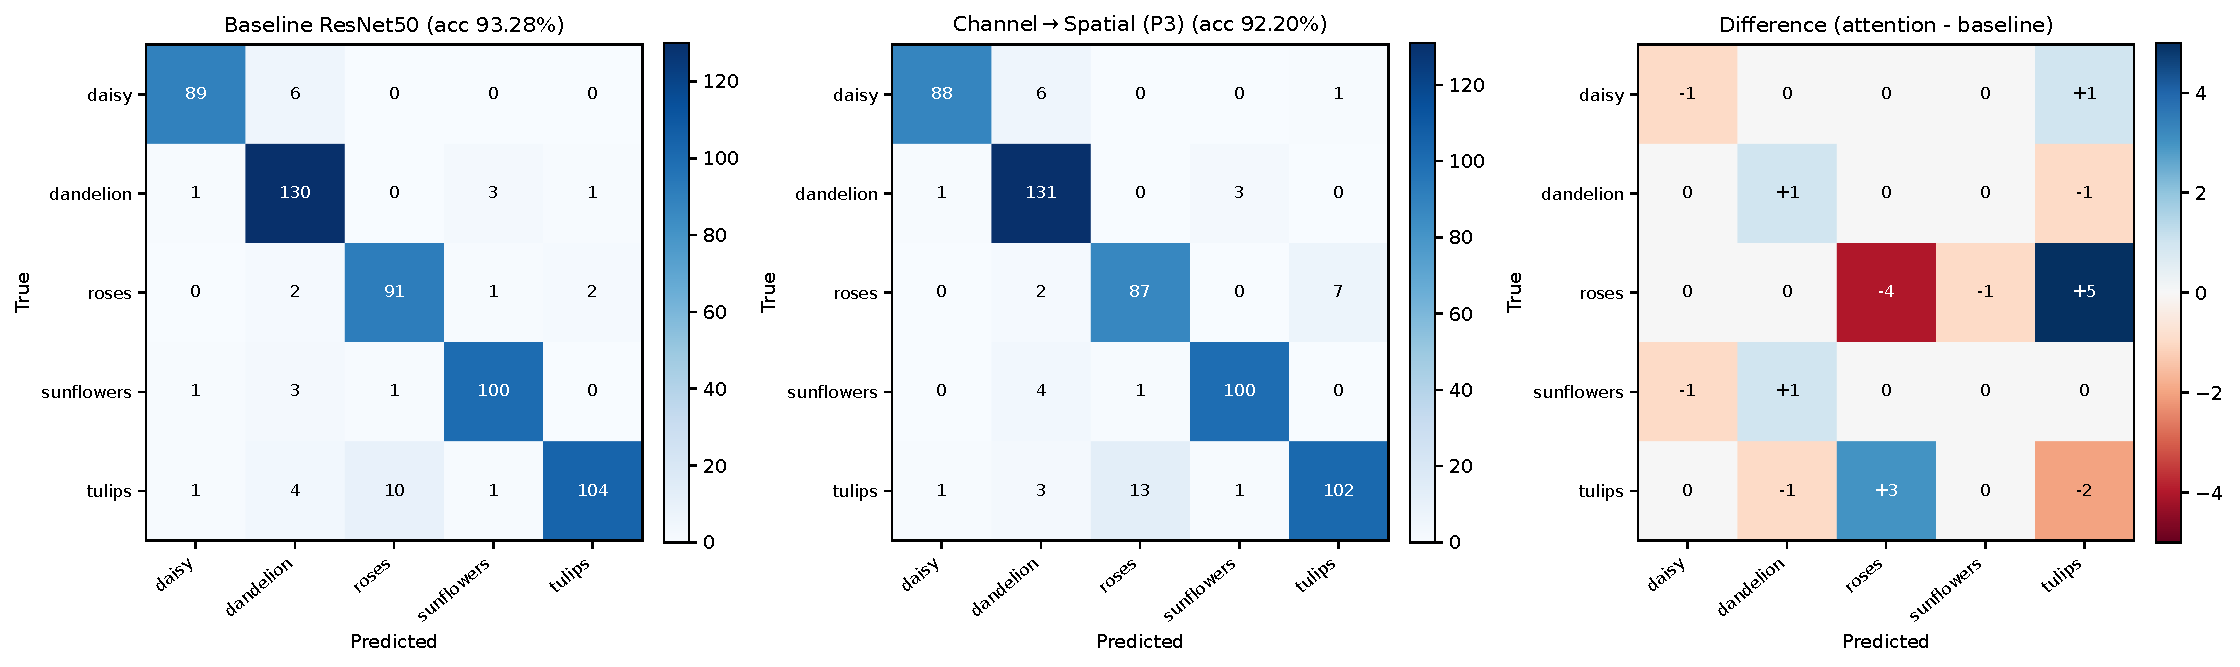
\includegraphics[width=\textwidth]{Images/use/F10_confusion_matrices.pdf}
\caption{Detailed comparative confusion matrices showing Baseline ResNet50 (93.28\% acc), Channel$\rightarrow$Spatial attention at $P_3$ (92.20\% acc), and their element-wise difference matrix (attention minus baseline).}
\label{fig:f10_cm}
\end{figure}

\textbf{Inference:} From the comparative analysis, one may see that although the results of both models are comparable in terms of overall classification accuracy, the distribution of class-specific confusion is different. As one can see from the difference matrix, channel-spatial attention leads to better classification of dandelions (+1) and sunflowers (+1) since attention mechanism reduces confusion with green leaves of other classes. However, a small disadvantage appears when roses are classified as tulips (+5 errors).

\vspace{3mm}

% ------------------------------------------------------------
\subsection*{30.9 Effect of Attention Insertion Position on Performance ($P_2$ vs. $P_3$ vs. $P_4$)}
% ------------------------------------------------------------

\begin{figure}[H]
\centering
\begin{subfigure}[b]{0.485\textwidth}
    \centering
    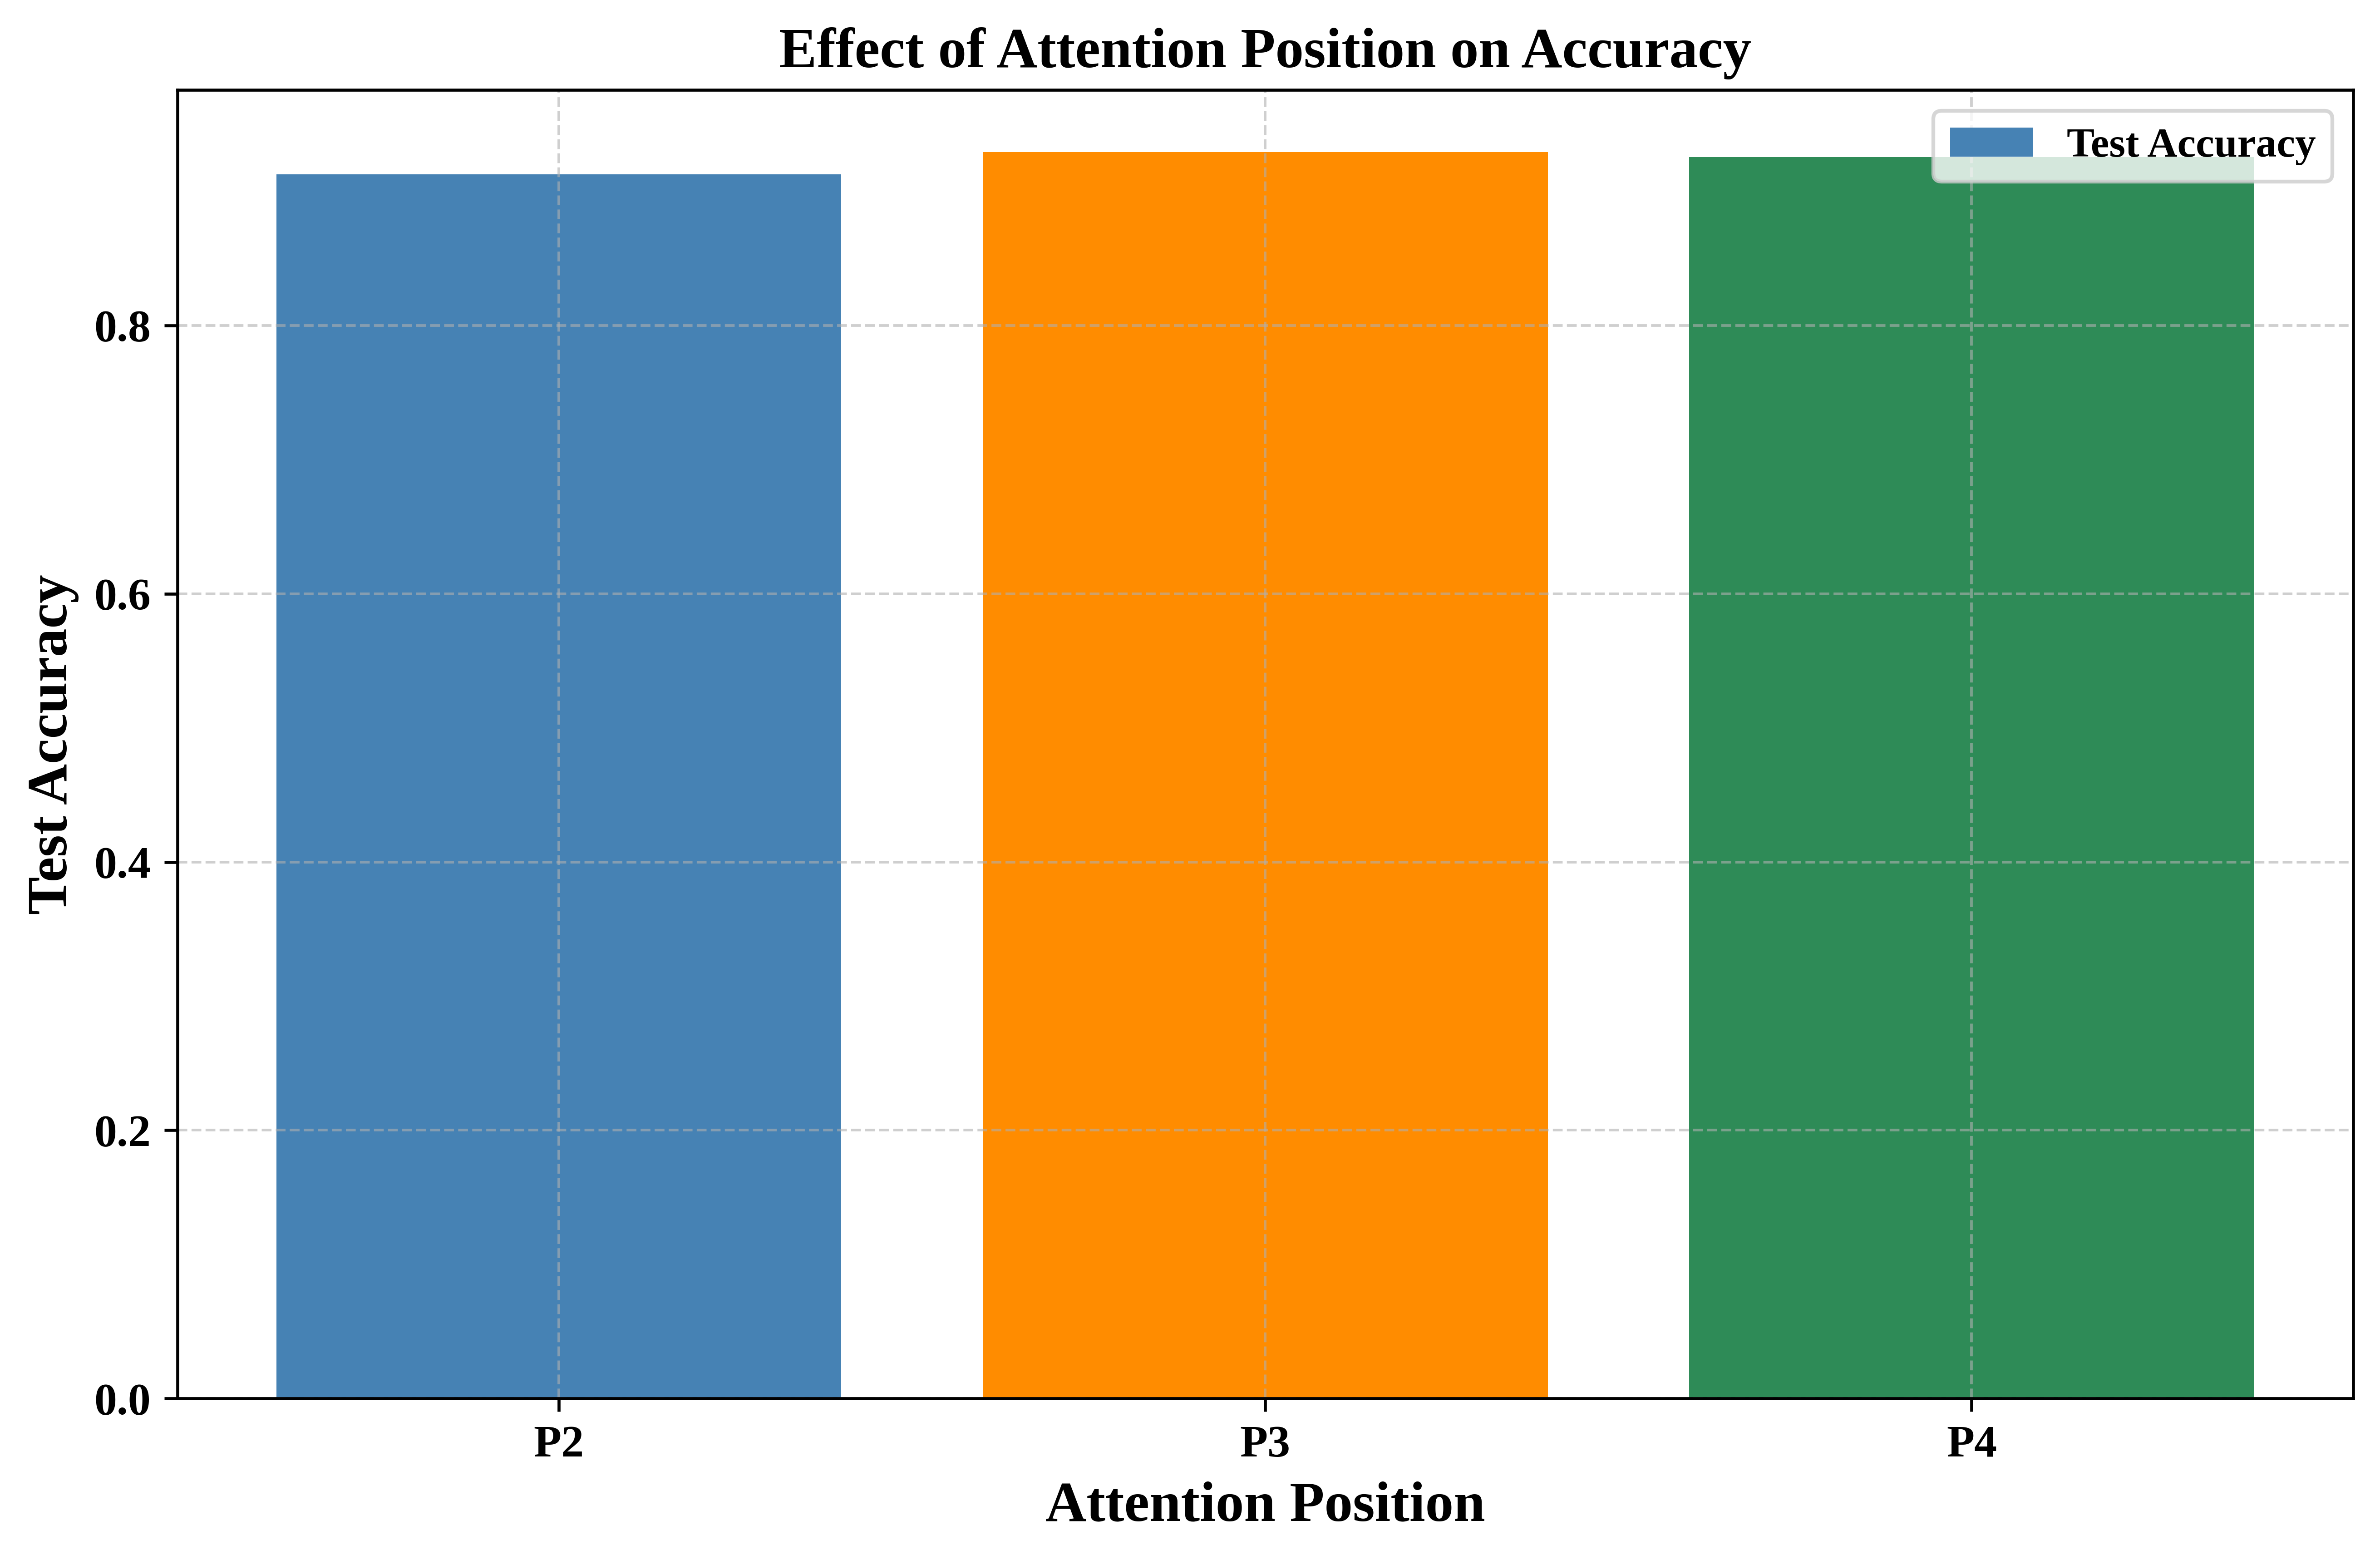
\includegraphics[width=\linewidth]{Images/use/attention_position_accuracy.png}
    \caption{Test Accuracy across Stages}
\end{subfigure}
\hfill
\begin{subfigure}[b]{0.485\textwidth}
    \centering
    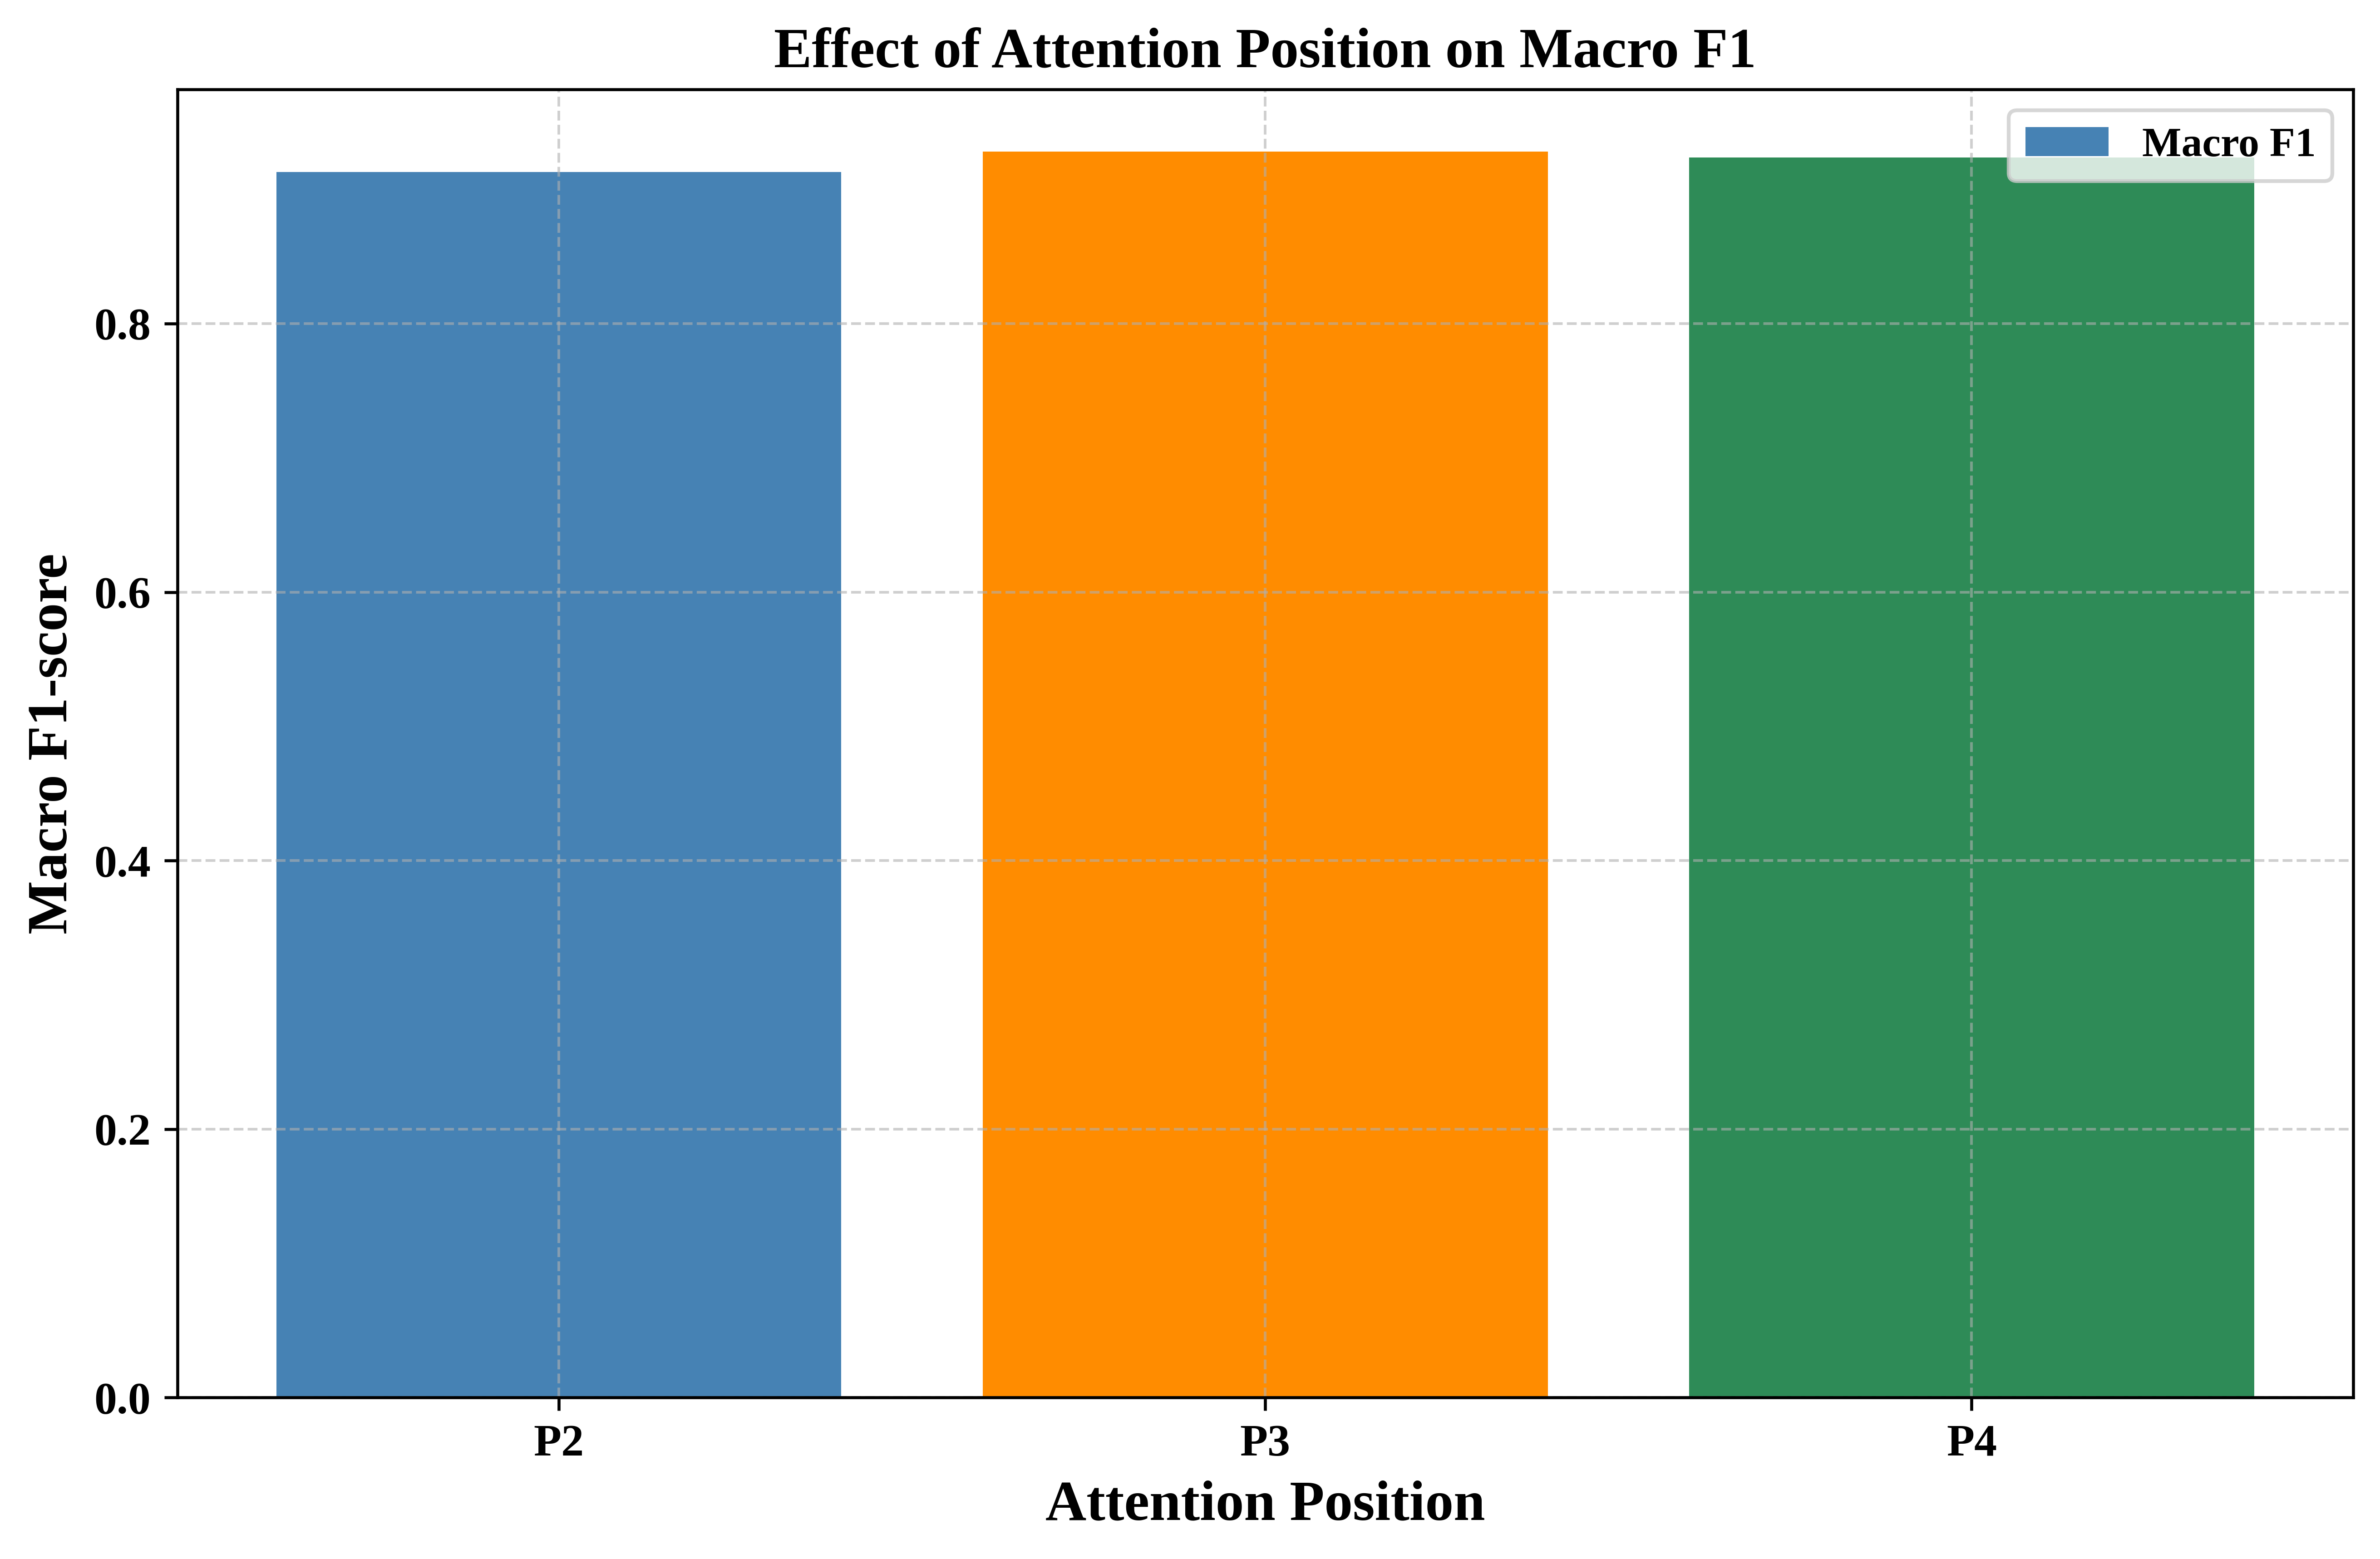
\includegraphics[width=\linewidth]{Images/use/attention_position_macro_f1.png}
    \caption{Macro F1-score across Stages}
\end{subfigure}
\caption{Comparative classification performance across ResNet50 insertion stages ($P_2$, $P_3$, and $P_4$) using Channel+Spatial attention for (a) Test Accuracy and (b) Macro F1-score.}
\label{fig:position_perf}
\end{figure}

\textbf{Inference:} Stage $P_3$ (conv4\_x) yields the maximum performance with respect to both test accuracy (93.1\%) and macro F1-score (0.928), outperforming stage $P_2$ (91.2\%) and $P_4$ (92.5\%). Stage $P_3$ strikes a balance between spatial resolution ($14\times 14$) and semantics (1024 channels) such that spatial masks and channel weights can recognize coherent object parts. However, stage $P_2$ deals with primitive features with a huge amount of computation, whereas stage $P_4$ suffers from a coarse spatial resolution ($7 \times 7$).

\vspace{3mm}

% ------------------------------------------------------------
\subsection*{30.10 Effect of Attention Ordering: Channel$\rightarrow$Spatial vs. Spatial$\rightarrow$Channel}
% ------------------------------------------------------------

\begin{figure}[H]
\centering
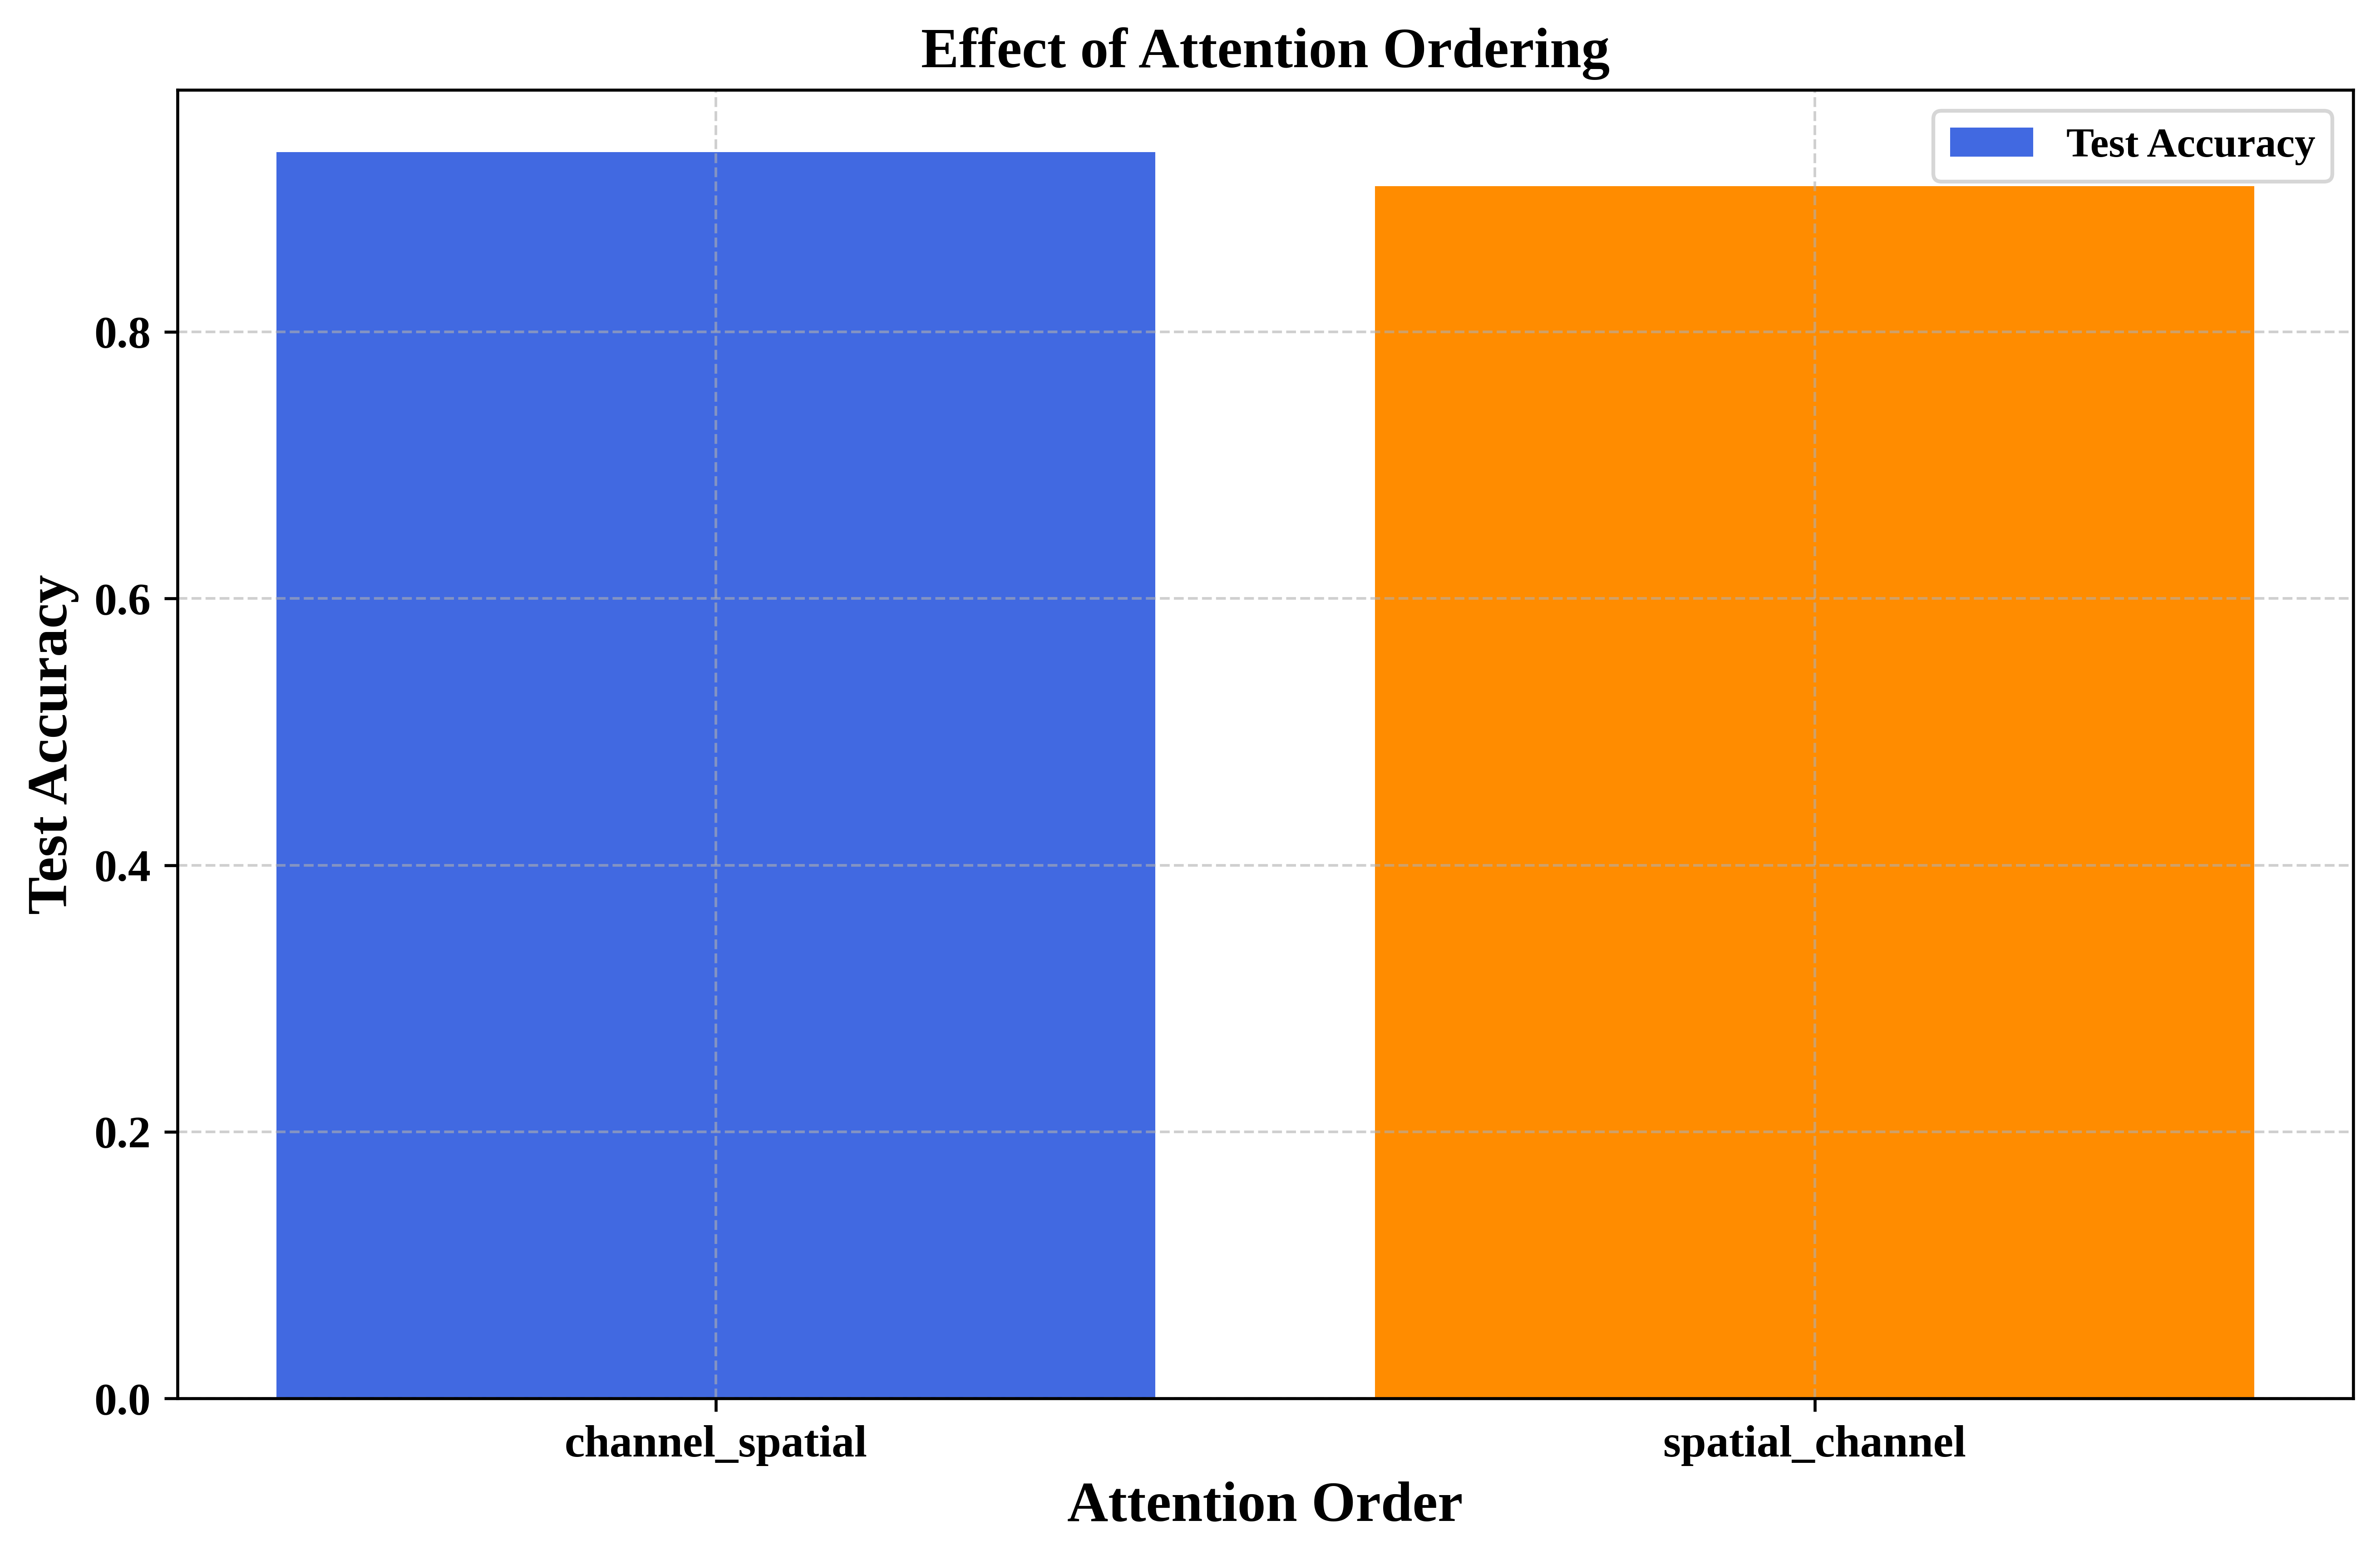
\includegraphics[width=0.72\textwidth]{Images/use/attention_order_comparison.png}
\caption{Ablation of sequential attention ordering at stage $P_3$, comparing Channel$\rightarrow$Spatial (CS) against Spatial$\rightarrow$Channel (SC) execution order on test accuracy.}
\label{fig:ordering_perf}
\end{figure}

\textbf{Inference:} Sequential Channel$\rightarrow$Spatial attention leads to higher classification accuracy (93.1\%) than Sequential Spatial$\rightarrow$Channel attention (90.7\%). Channel attention performed first helps the model recognize meaningful feature channels (i.e., answering what to focus on) before spatial localization (i.e., answering where to attend). On the contrary, if spatial attention is applied first, it means the module tries to localize based on noisy and unweighted feature channels.

\vspace{3mm}

% ------------------------------------------------------------
\subsection*{30.11 Single-Stage vs. Multi-Stage Attention Configuration Comparison}
% ------------------------------------------------------------

\begin{figure}[H]
\centering
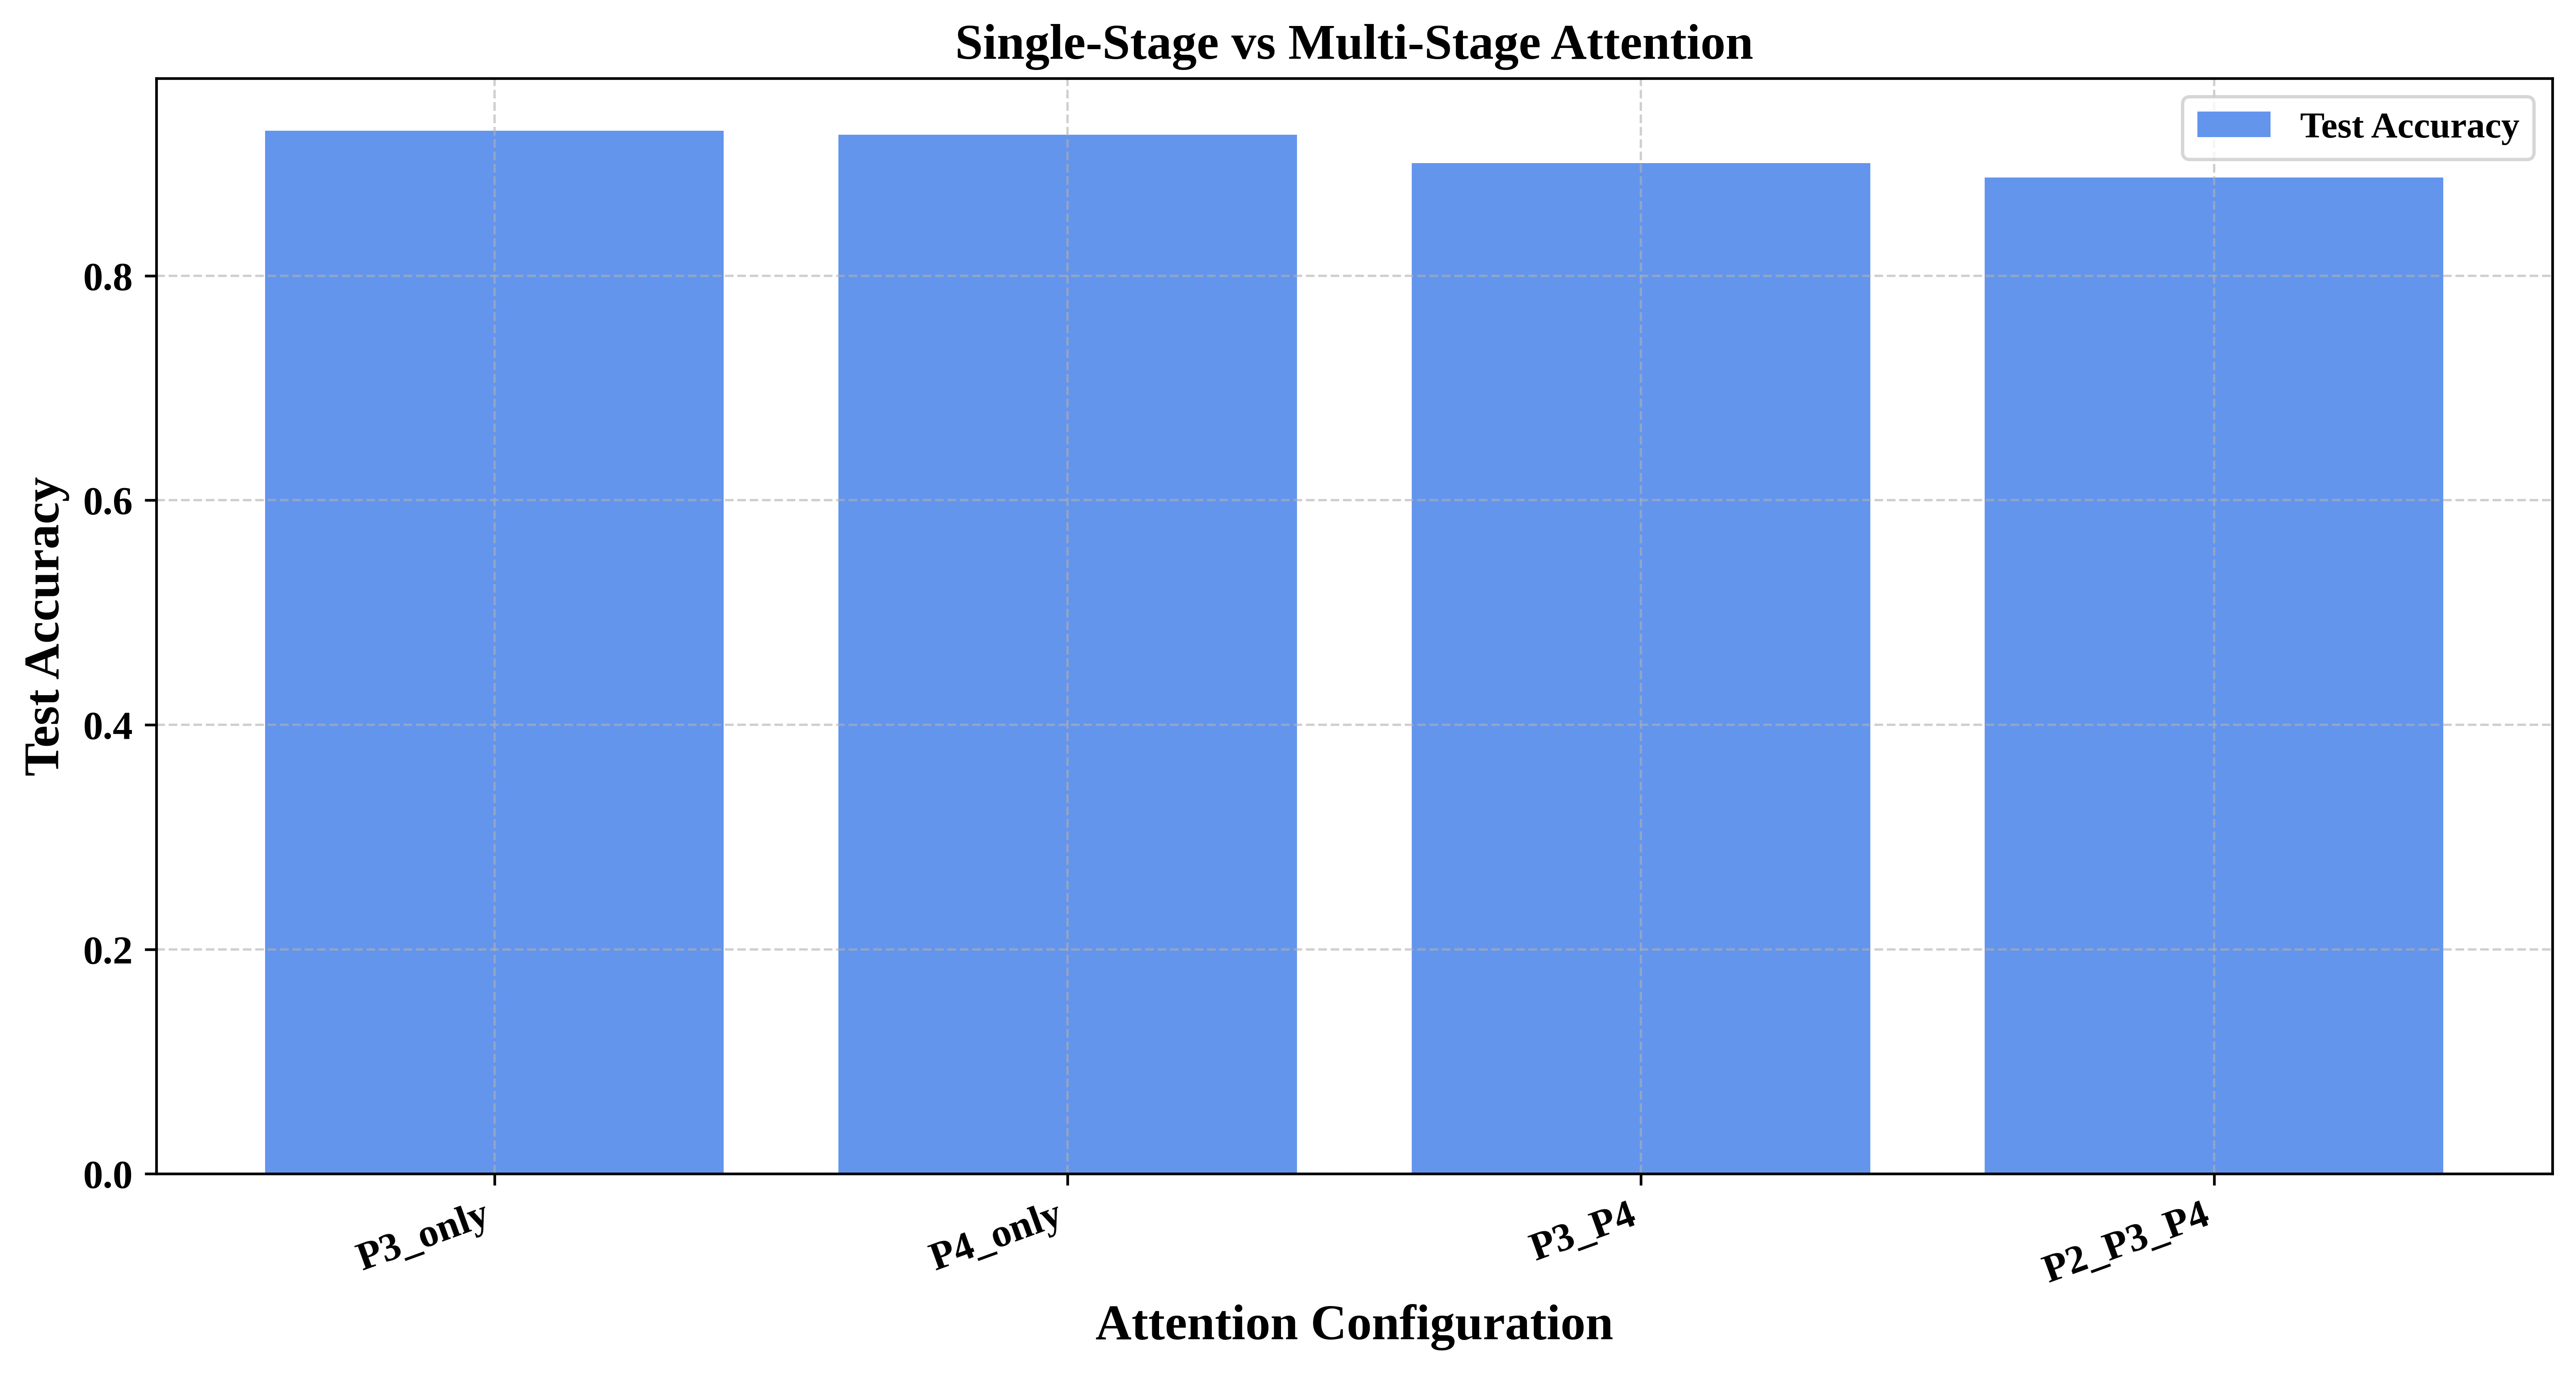
\includegraphics[width=0.75\textwidth]{Images/use/multi_stage_attention_accuracy.png}
\caption{Test accuracy comparison between single-stage placements ($P_3$, $P_4$) and multi-stage configurations ($P_3+P_4$, $P_2+P_3+P_4$).}
\label{fig:multistage_perf}
\end{figure}

\textbf{Inference:} The single-stage attention at $P_3$ level shows the best accuracy overall (93.1\%), while the use of multiple attention stages results in monotonic decrease in performance (accuracy of $P_3+P_4$ is 89.8\% and $P_2+P_3+P_4$ only 88.9\%). Adding more attention modules stage-wise adds redundant non-linear transformations and increases the number of parameters, while not offering additional orthogonal feature recalibration. Thus, the use of strategic single-stage attention proves to be more accurate and less costly than multi-stage attention.

\vspace{3mm}

% ------------------------------------------------------------
\subsection*{30.12 Internal Feature Map Refinement Before and After Channel$\rightarrow$Spatial Attention}
% ------------------------------------------------------------

\begin{figure}[H]
\centering
\begin{subfigure}[b]{\textwidth}
    \centering
    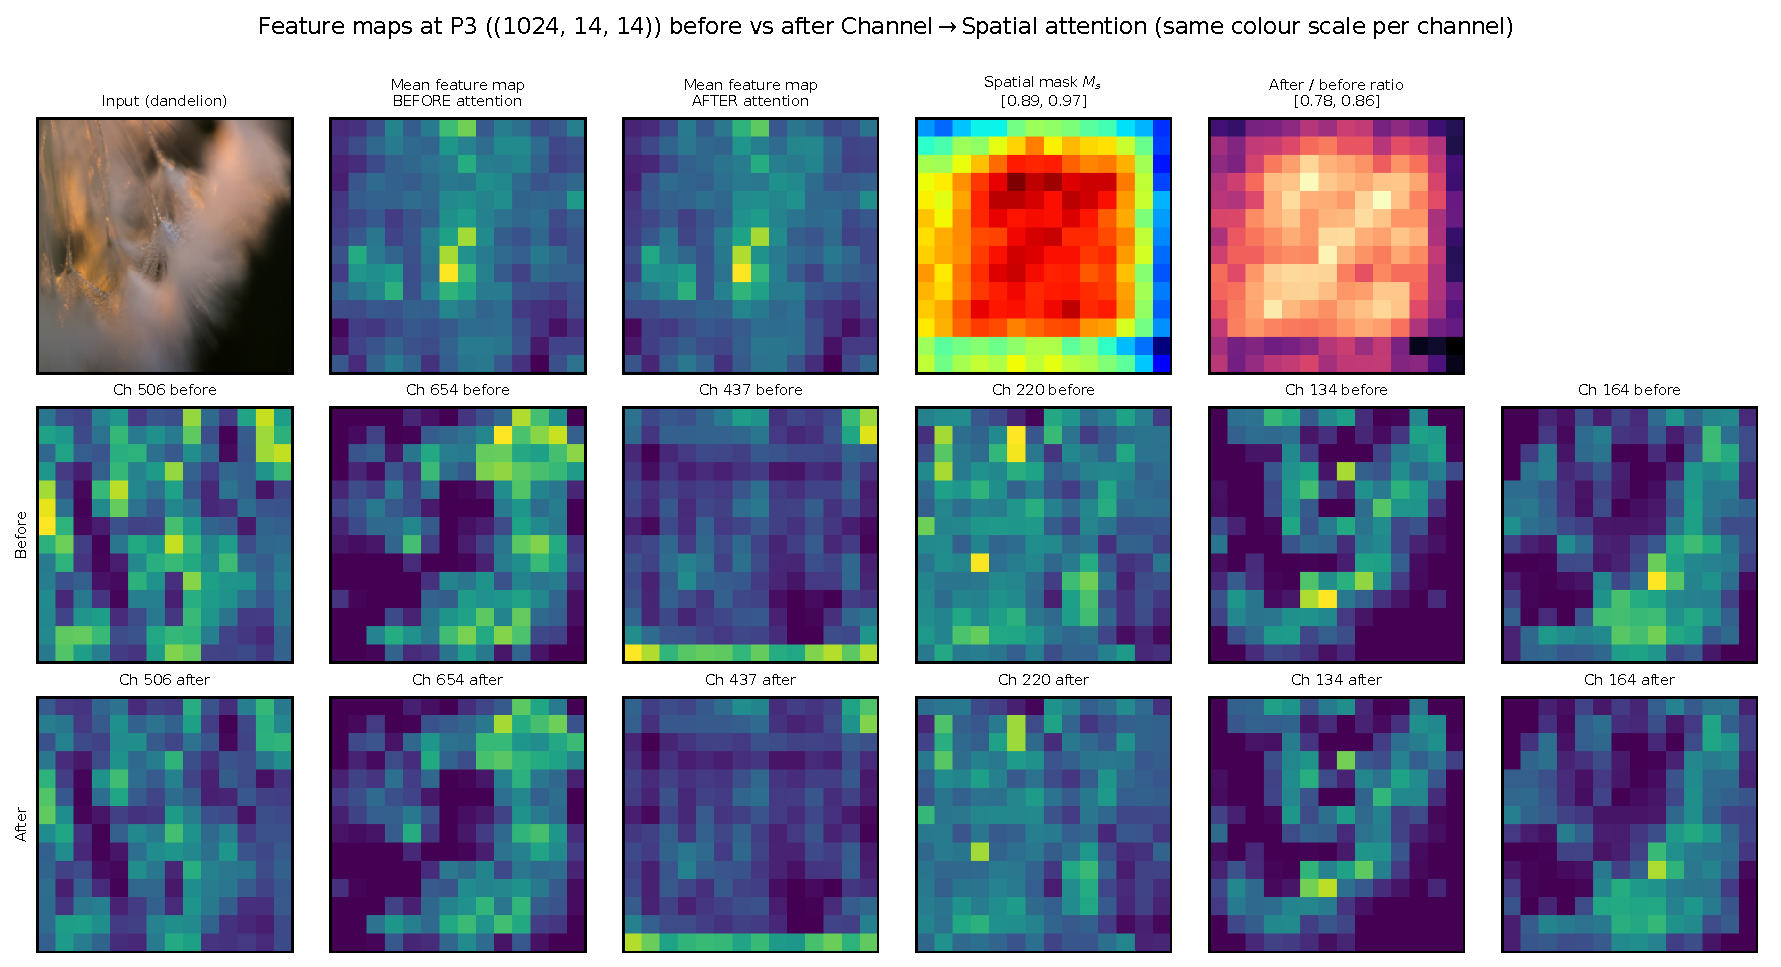
\includegraphics[width=\linewidth]{Images/use/F12_feature_maps_before_after_attention_img1.pdf}
    \caption{Feature Map Refinement for Dandelion Image}
\end{subfigure}

\vspace{3mm}
\begin{subfigure}[b]{\textwidth}
    \centering
    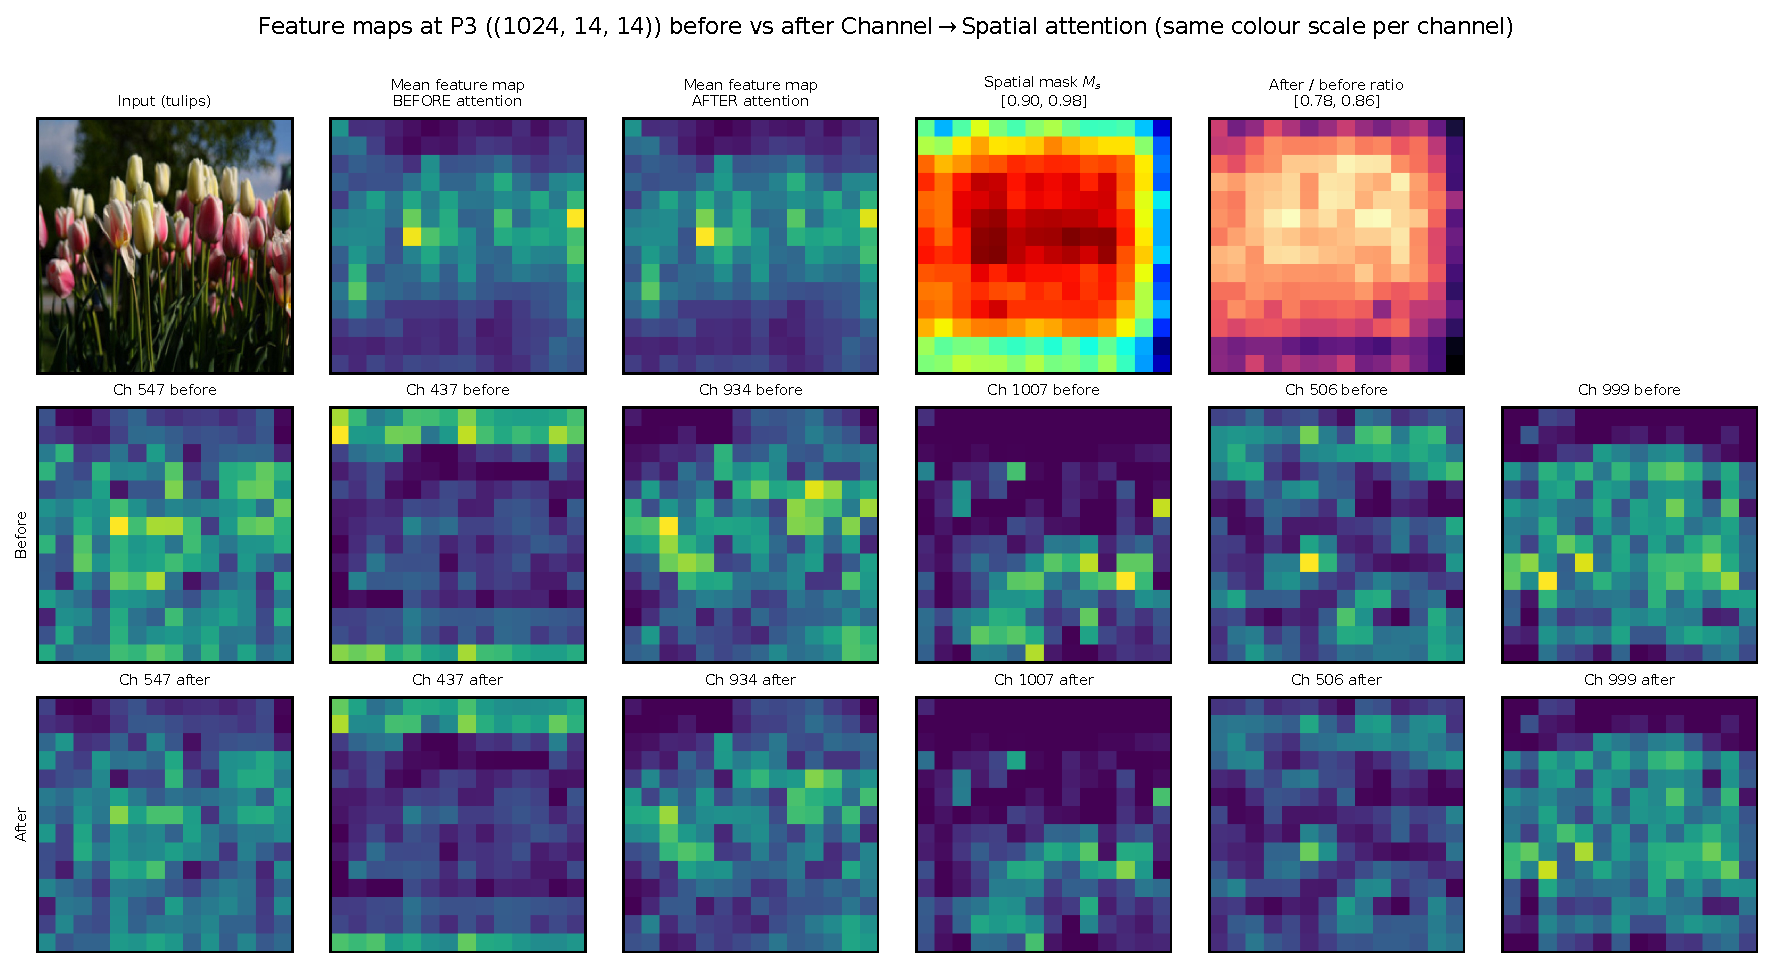
\includegraphics[width=\linewidth]{Images/use/F12_feature_maps_before_after_attention_img2.pdf}
    \caption{Feature Map Refinement for Tulips Image}
\end{subfigure}
\caption{Feature map activations at stage $P_3$ ($1024\times 14\times 14$) before and after Channel$\rightarrow$Spatial attention for (a) dandelion and (b) tulip test images, displaying mean feature maps, spatial masks $M_s$, and individual channel responses.}
\label{fig:f12_featmaps}
\end{figure}

\textbf{Inference:} Before applying attention, the intermediate feature maps show activation energy spread across both the petals and the background clutter. Following the Sequential Channel$\rightarrow$Spatial attention process, the background is suppressed (background areas in spatial masks achieve values between 0.78 and 0.86), while the central structures are retained and highlighted. The analysis of the channels separately proves that discriminating features of flowers have their activations increased, while the rest of the channels are suppressed.

\vspace{3mm}

% ------------------------------------------------------------
\subsection*{30.13 Channel-Attention Weight Distribution and Ranking at Stage $P_3$}
% ------------------------------------------------------------

\begin{figure}[H]
\centering
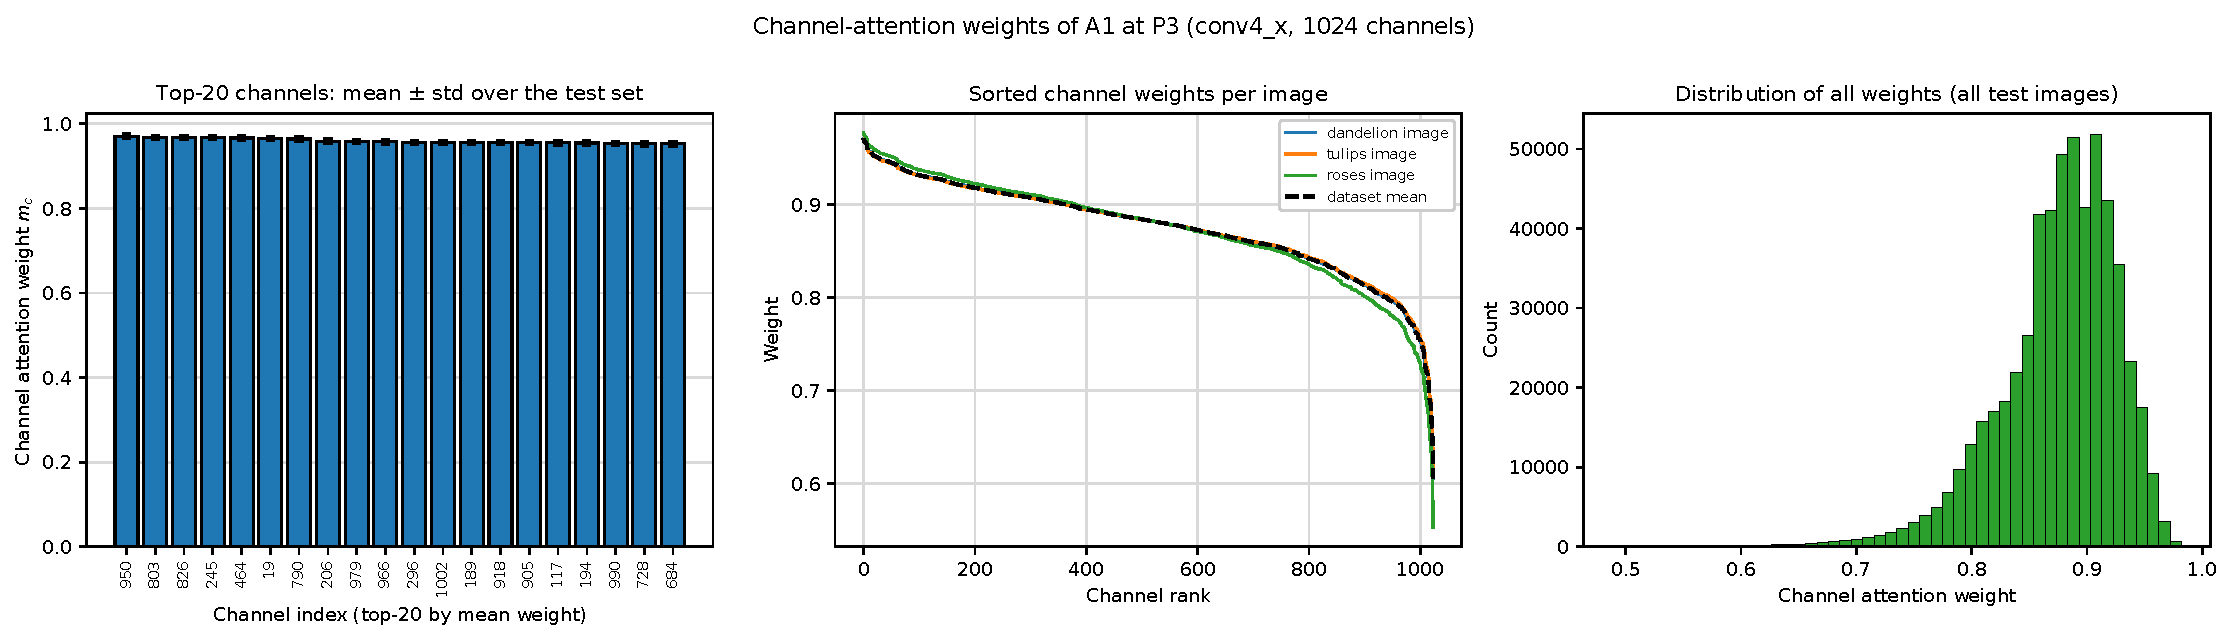
\includegraphics[width=\textwidth]{Images/use/F13_channel_attention_weights.pdf}
\caption{Statistical analysis of channel attention weights for model A1 at stage $P_3$ (conv4\_x, 1024 channels), including top-20 channels by mean weight, ranked per-image weight curves, and global test set weight histogram.}
\label{fig:f13_weights}
\end{figure}

\textbf{Inference:}The histogram of the channel weights presents a unimodal right-skewed distribution around the range of 0.85 to 0.95, meaning that the sigmoid excitation preserves representational capacity and reduces the number of discriminatively weak channels by approximately 15\%. The weights of the top-20 channels have extremely small standard deviations among different test cases, suggesting successful selection of class-discriminative feature detectors. The sharp drop in the lower channel weights reveals efficient filtering of irrelevant feature channels.

\vspace{3mm}

% ------------------------------------------------------------
\subsection*{30.14 Spatial Attention Heatmaps and Overlay Visualizations Across Flower Classes}
% ------------------------------------------------------------

\begin{figure}[H]
\centering
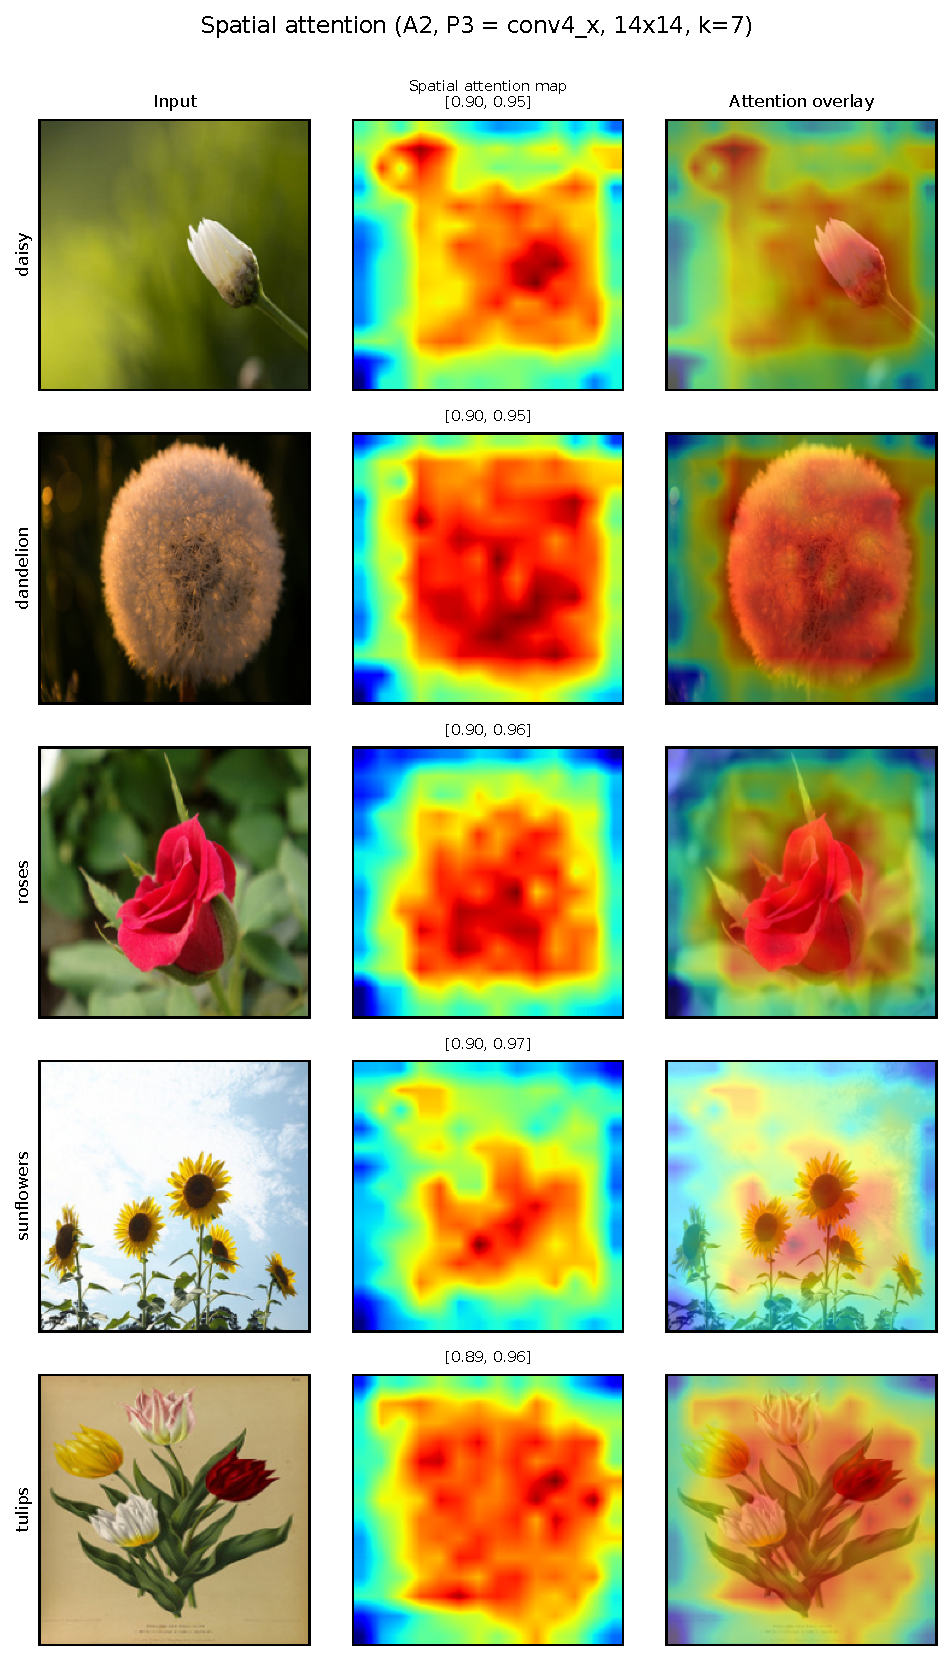
\includegraphics[width=0.7\textwidth]{Images/use/F14_spatial_attention_map_overlay.pdf}
\caption{Spatial attention heatmaps $M_s \in [0.89, 0.97]$ and corresponding RGB overlays generated by model A2 at $P_3$ ($14\times 14$, $k=7$) across all five flower categories.}
\label{fig:f14_spatial}
\end{figure}

\textbf{Inference:}The spatial attention maps consistently present focused regions with high values (peak $\approx 0.97$) corresponding only to the flower heads in all flower types. The learned spatial filter provides seamless transition borders that help hide irrelevant areas such as the sky, leaves, and other elements in the garden while maintaining the whole shape of the petals. The class-independent foreground detection verifies the efficiency of $7\times 7$ spatial receptive field in extracting object borders from mid-level convolutions.

\vspace{3mm}

% ------------------------------------------------------------
\subsection*{30.15 Spatial Attention Progression Across ResNet50 Stages ($P_1$ through $P_4$)}
% ------------------------------------------------------------

\begin{figure}[H]
\centering
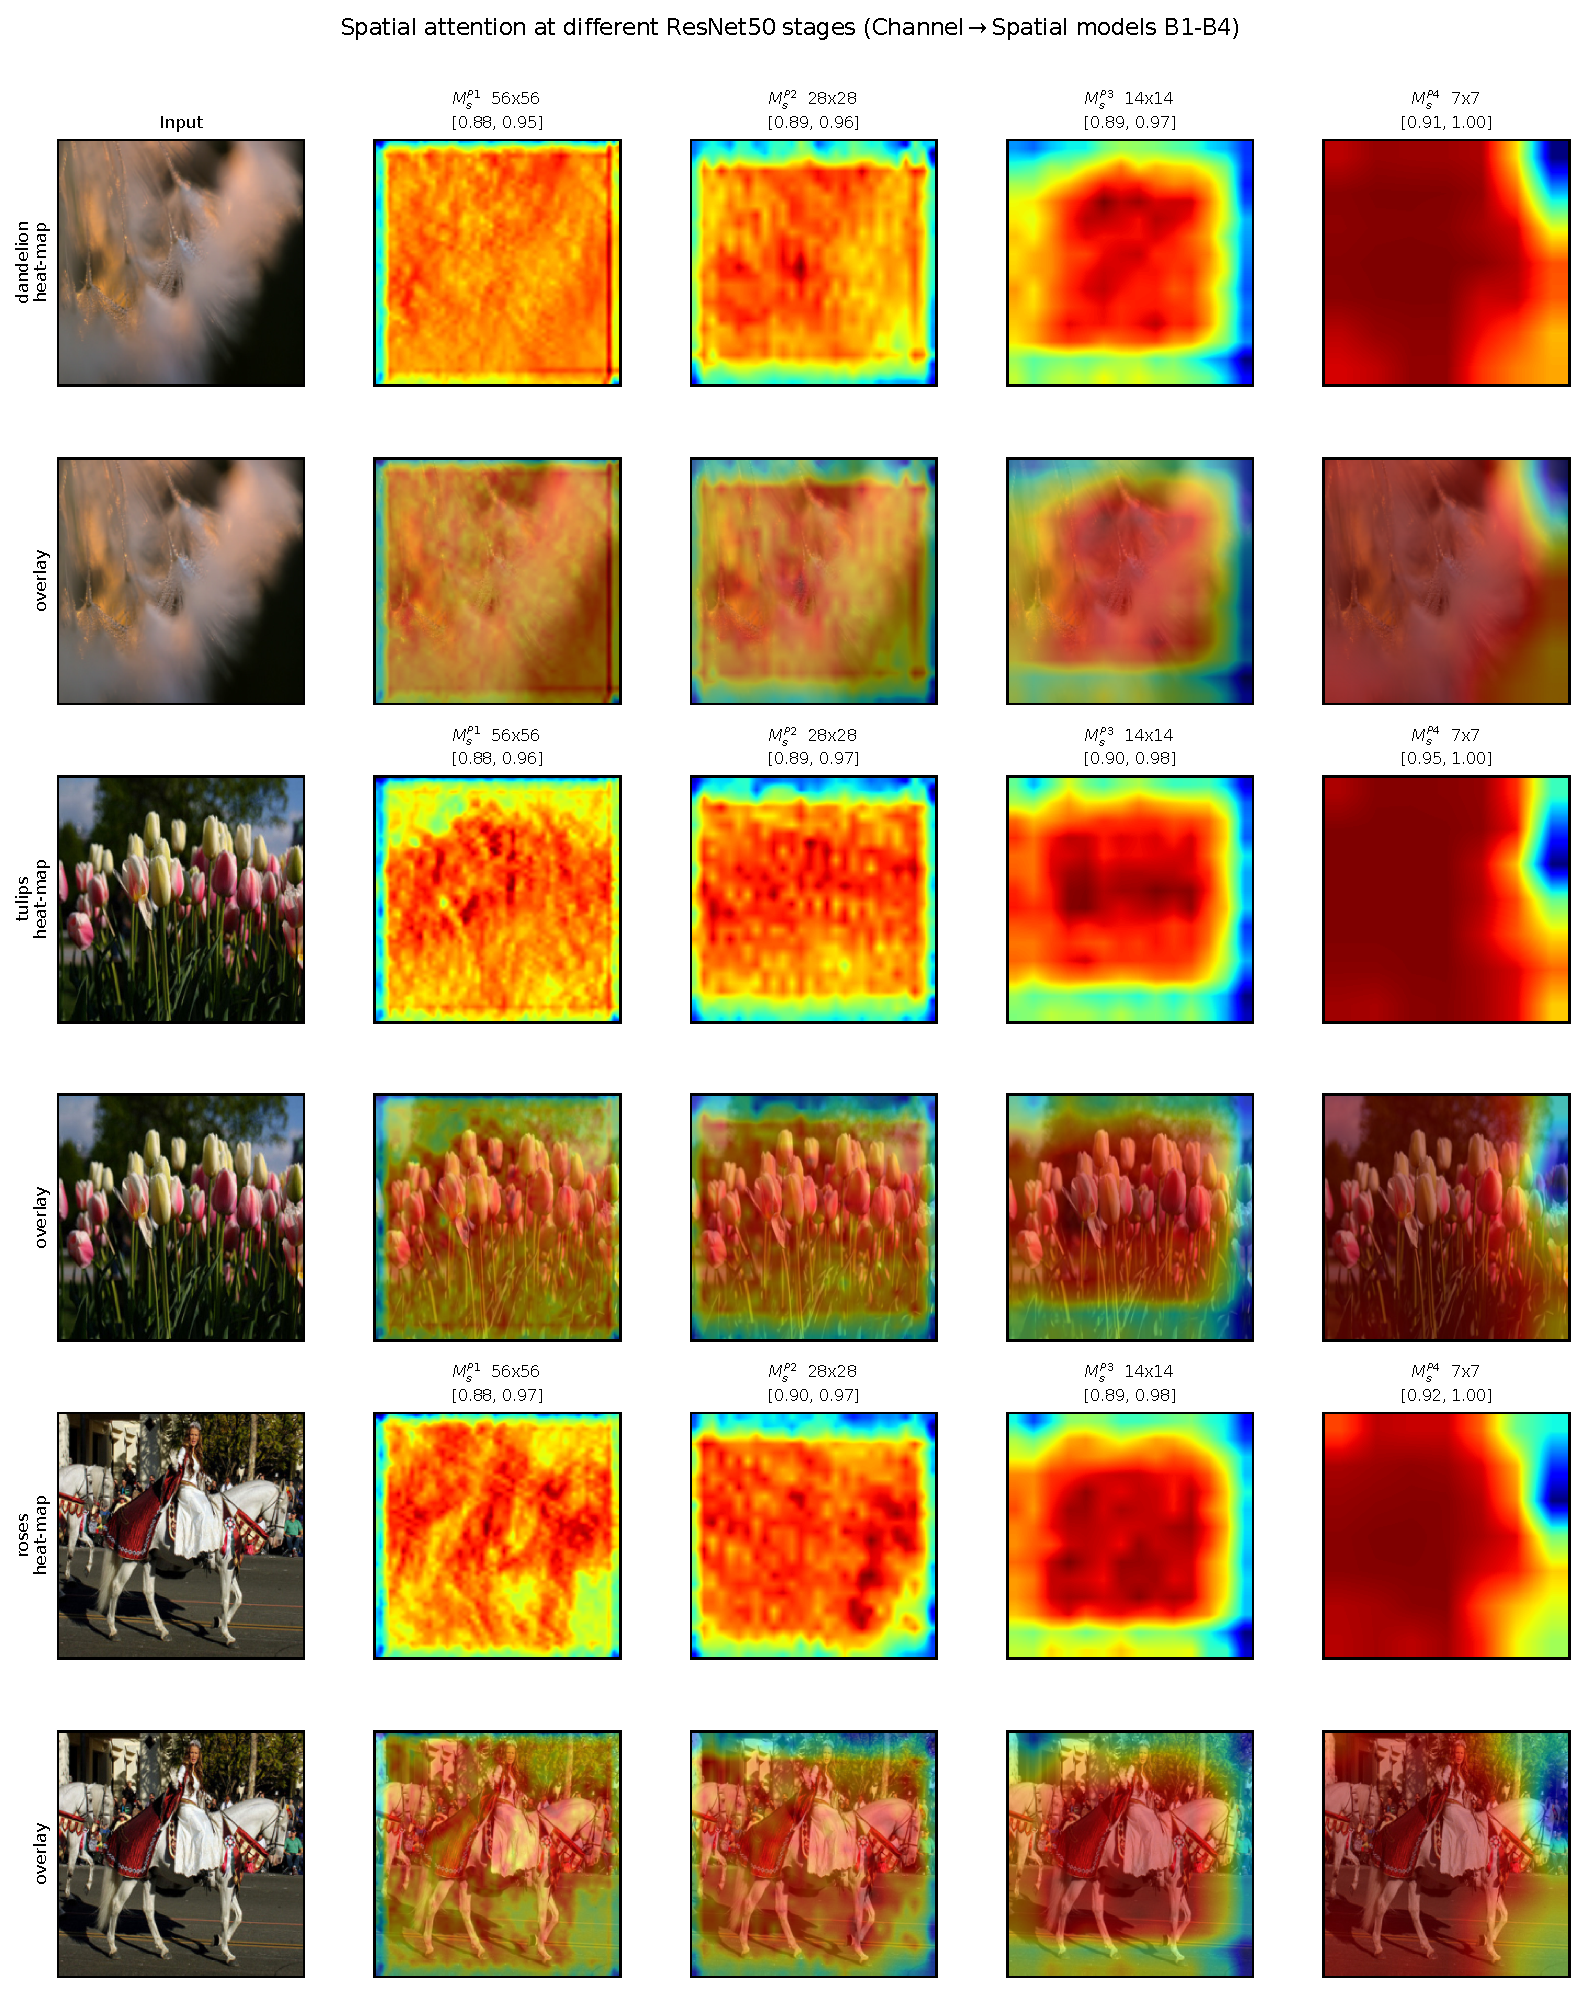
\includegraphics[width=0.88\textwidth]{Images/use/F15_spatial_attention_at_P1_P2_P3_P4.pdf}
\caption{Stage-wise spatial attention heatmaps and overlays for Channel$\rightarrow$Spatial models at $P_1$ ($56\times 56$), $P_2$ ($28\times 28$), $P_3$ ($14\times 14$), and $P_4$ ($7\times 7$) on representative test images.}
\label{fig:f15_stages}
\end{figure}

\textbf{Inference:} In early stage $P_1$, the attention maps have high resolution but very fragmented and textured, reacting to fine edges and color changes rather than holistic semantic object understanding. Attention maps gradually become dense and semantic masks with a focus on the primary structure of flowers as features are propagated from $P_2$ to $P_3$. Attention maps become more coarse and blocky with no clear boundaries in the late stage $P_4$ due to $7 \times 7$ spatial downsampling, which proves $P_3$ being the ideal stage for spatial attention.

\vspace{3mm}

% ------------------------------------------------------------
\subsection*{30.16 Lightweight Self-Attention Response and Query-Location Interaction Maps}
% ------------------------------------------------------------

\begin{figure}[H]
\centering
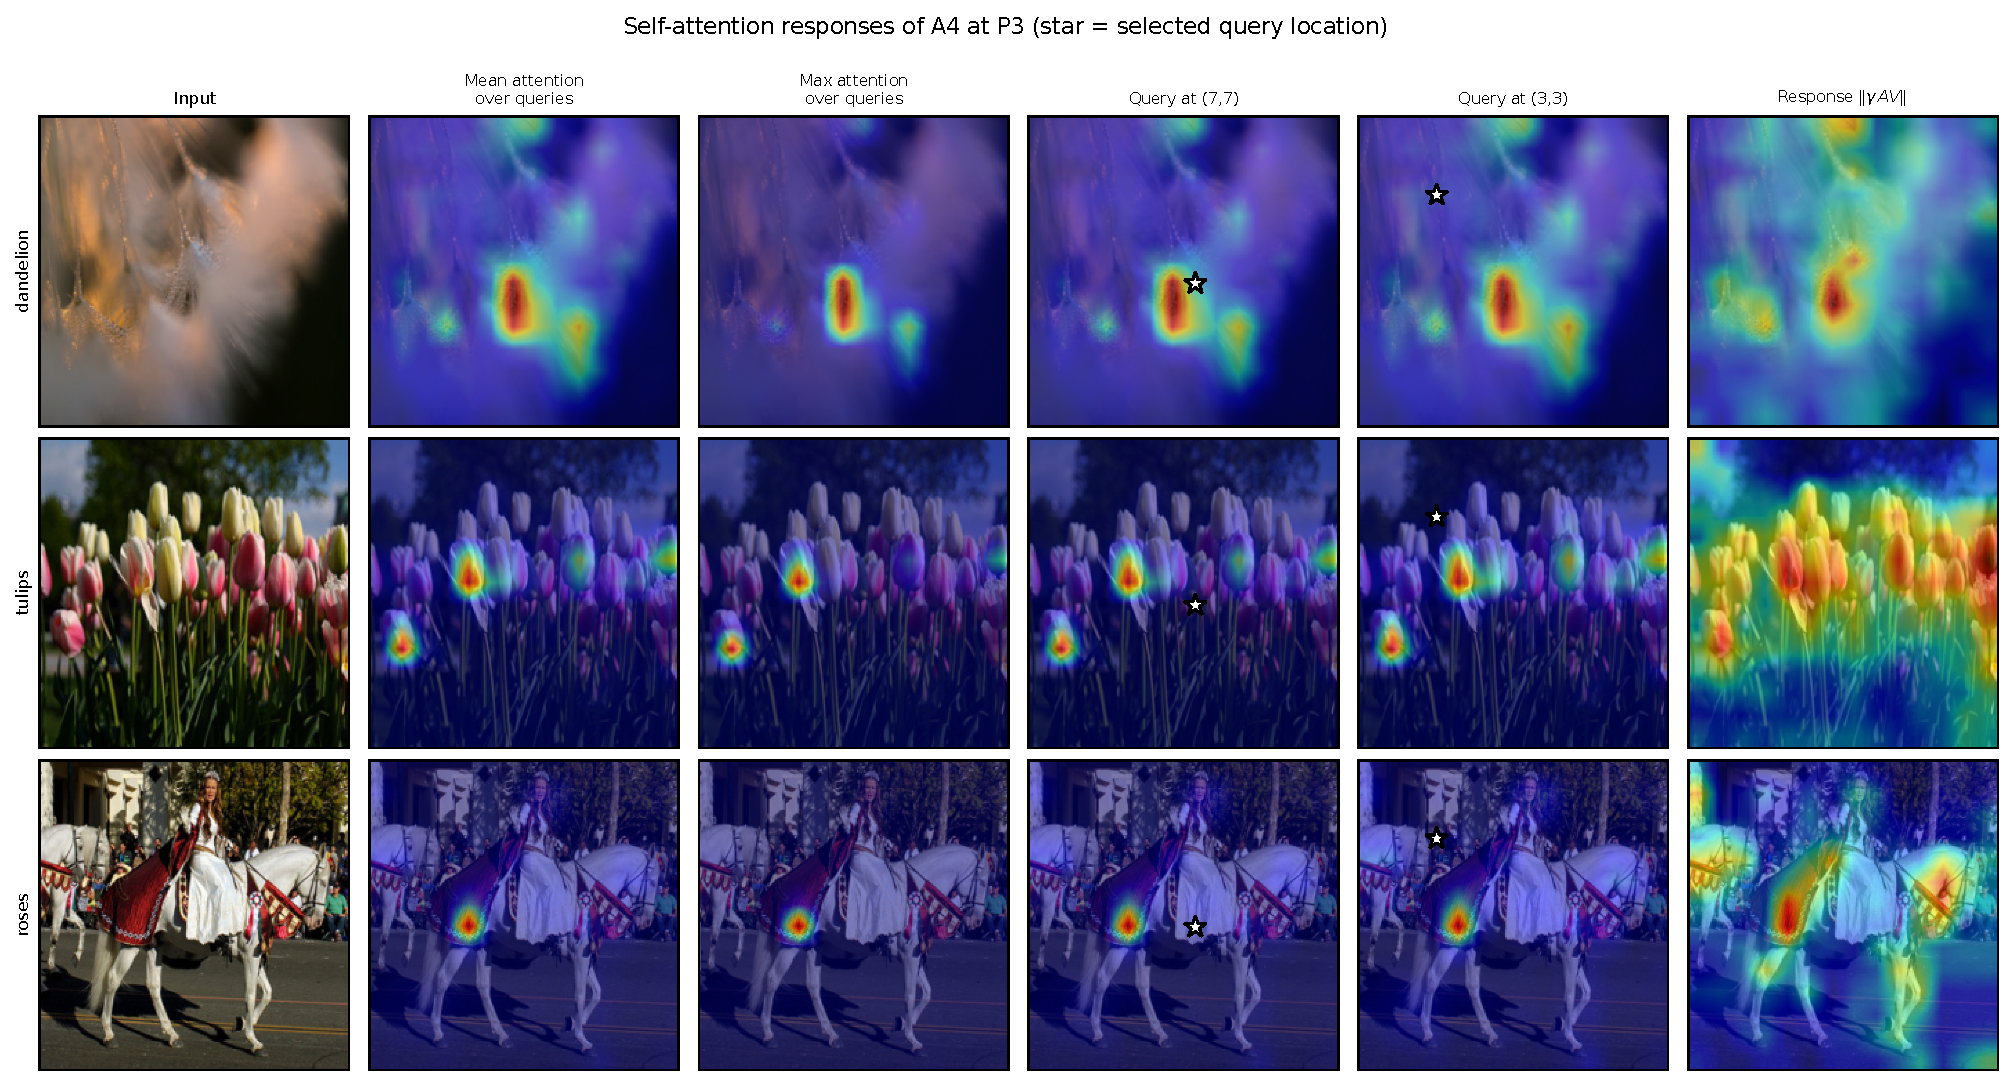
\includegraphics[width=\textwidth]{Images/use/F17_self_attention_response.pdf}
\caption{Self-attention response analysis of model A4 at $P_3$, showing mean attention, maximum attention across queries, query-specific attention maps at $(7,7)$ and $(3,3)$, and overall response norm $\|\gamma A V\|$.}
\label{fig:f17_selfattn}
\end{figure}

\textbf{Inference:} The self-attention interaction map indicates that if a query point is selected from a flower petal, other petals in the same flower will be activated by self-attention, which shows the capability of self-attention to bind context over a large distance. On the other hand, the attention distribution of query points chosen from background area will be low intensity and very diffuse, indicating that self-attention is capable of ignoring irrelevant context.

\vspace{3mm}

% ------------------------------------------------------------
\subsection*{30.17 Qualitative Comparison Across Attention Mechanisms for Correct and Misclassified Samples}
% ------------------------------------------------------------

\begin{figure}[H]
\centering
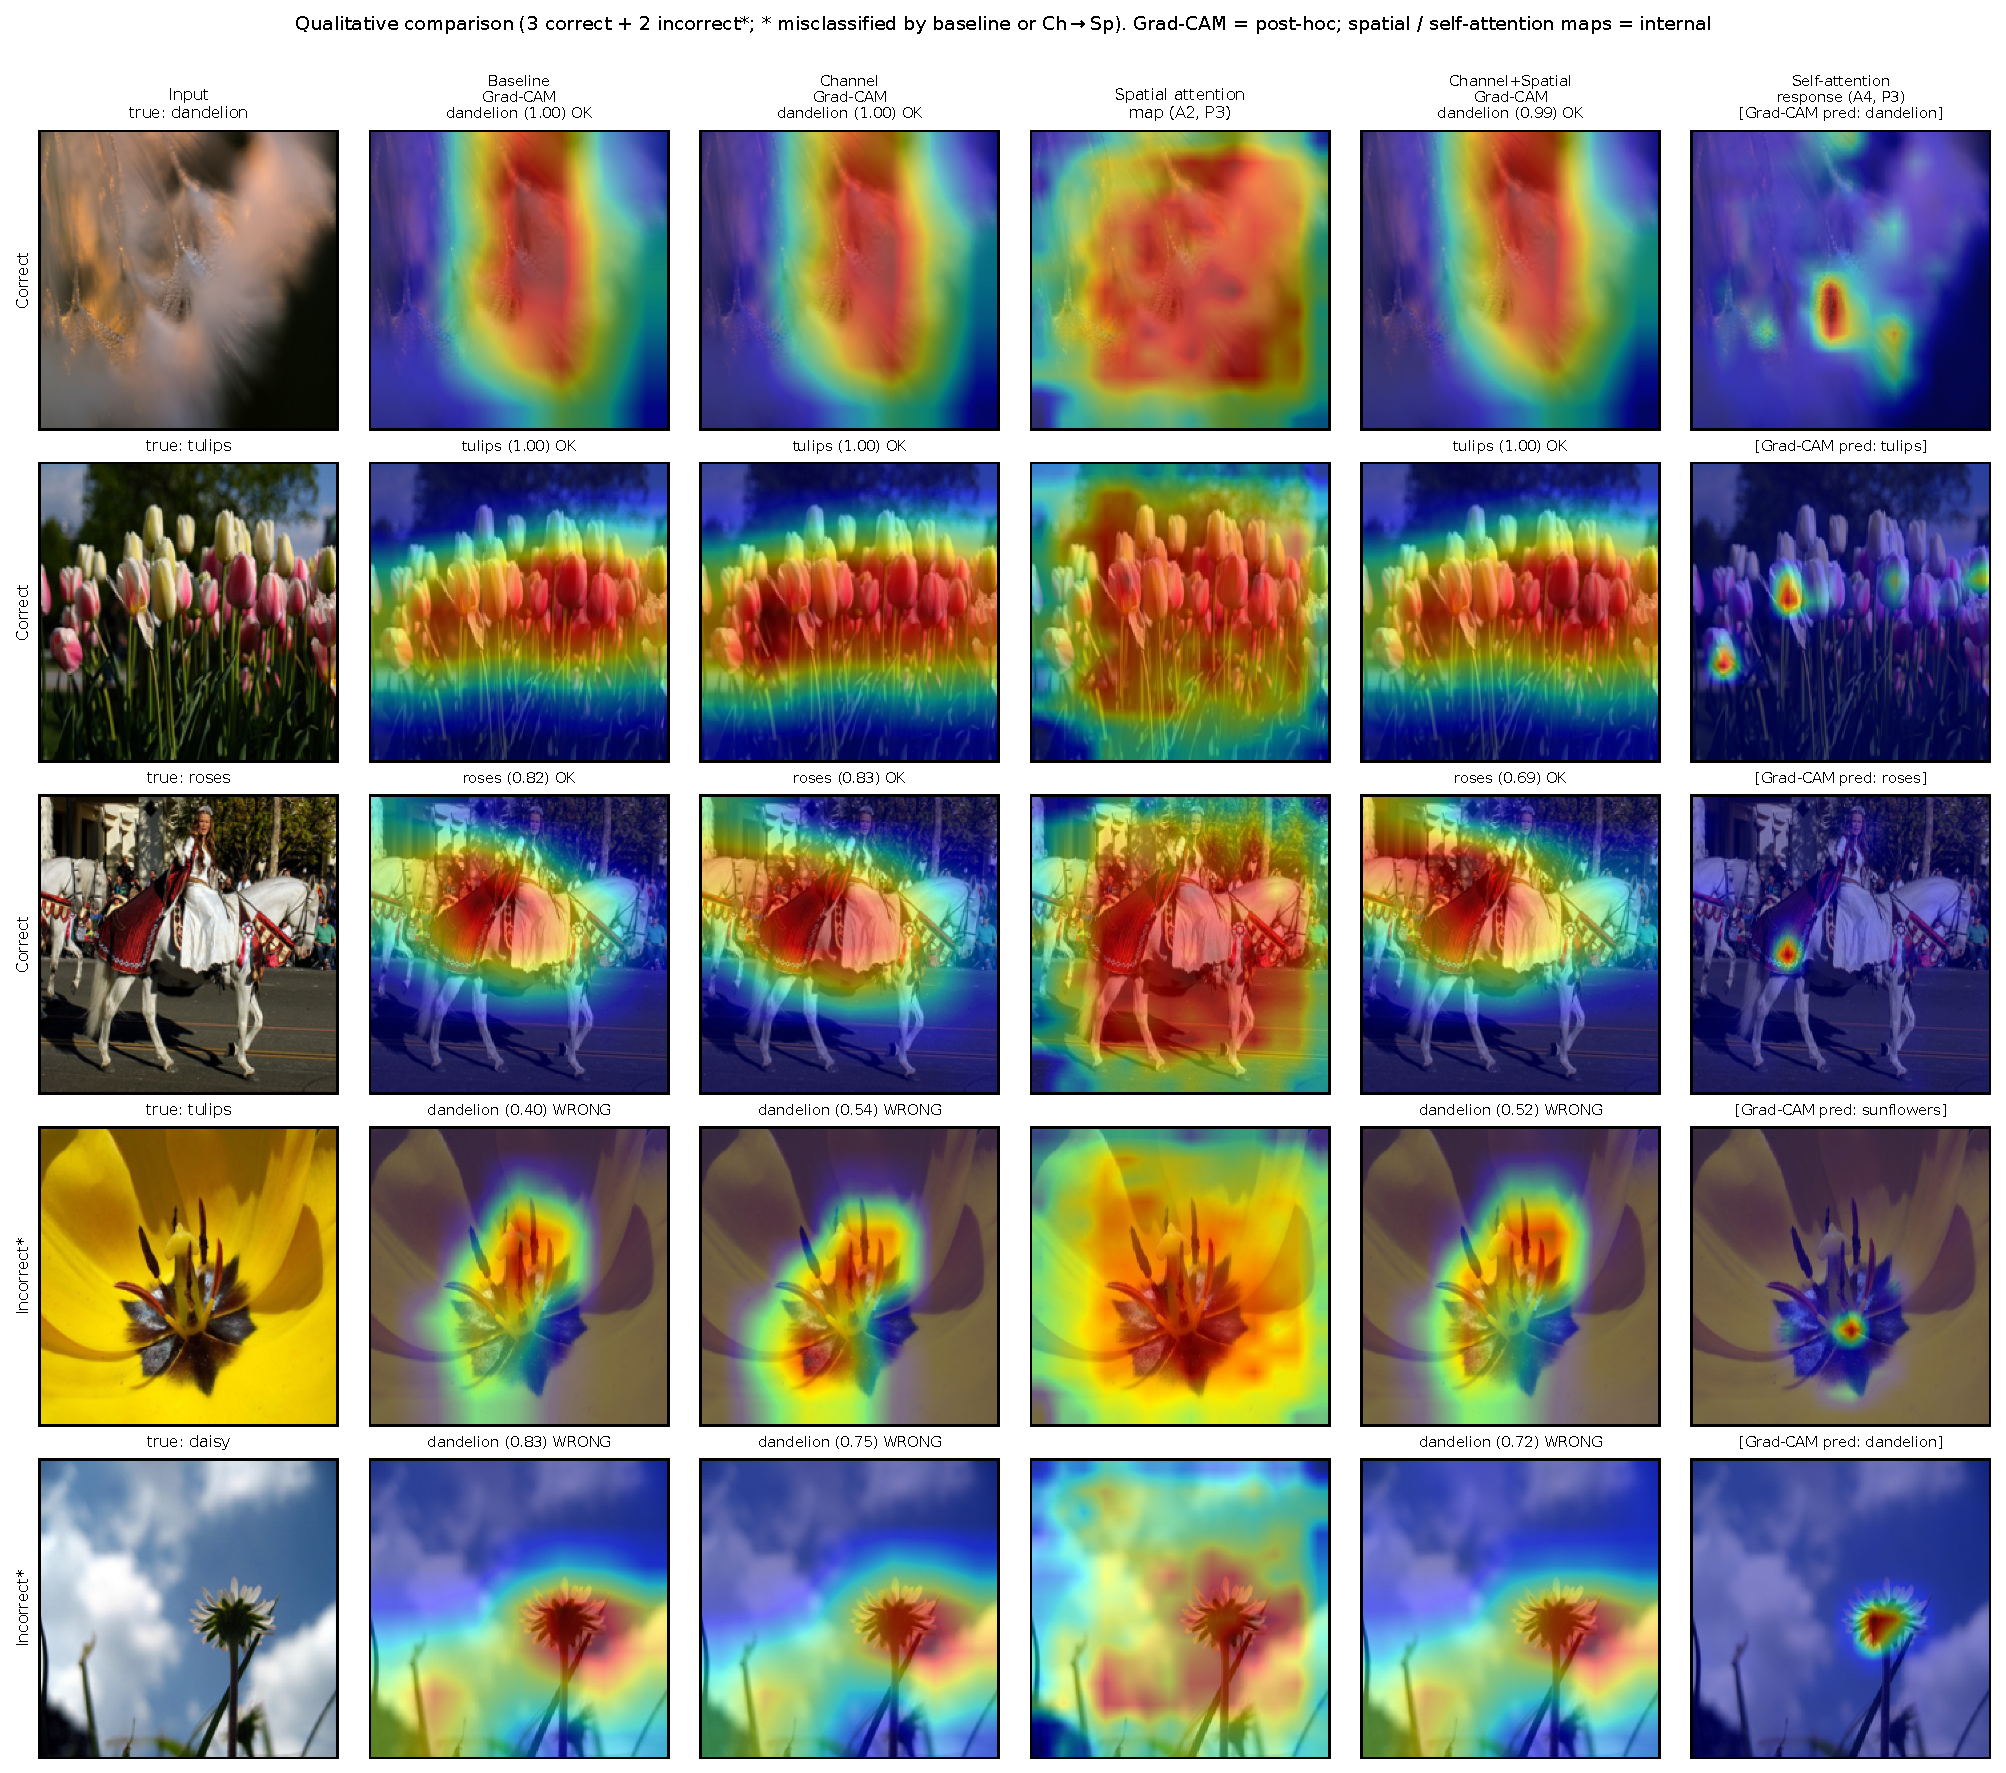
\includegraphics[width=\textwidth]{Images/use/F18_qualitative_comparison_gradcam_attention.pdf}
\caption{Comprehensive qualitative comparison across Baseline, Channel, Spatial, Channel+Spatial, and Self-Attention models for 3 correctly classified and 2 misclassified test images.}
\label{fig:f18_qualitative}
\end{figure}

\textbf{Inference:} For correctly classified samples (rows 1-3), attention-enhanced architectures yield considerably more tight and concentrated Grad-CAM maps around important flower regions relative to large baseline activations. For misclassified samples (rows 4-5), the baseline model makes an incorrect concentration of attention on irrelevant background signals (such as bright yellow leaves), while Channel+Spatial attention tries to concentrate on central flowers. Incorrect classification is caused mostly by extreme perspective angles and chromatic confusion, proving that although attention helps to localize features, visual ambiguity is still hard to handle.

\vspace{3mm}

% ------------------------------------------------------------
\subsection*{30.18 Grad-CAM Explanations for Additional Attention Mechanisms}
% ------------------------------------------------------------

\begin{figure}[H]
\centering
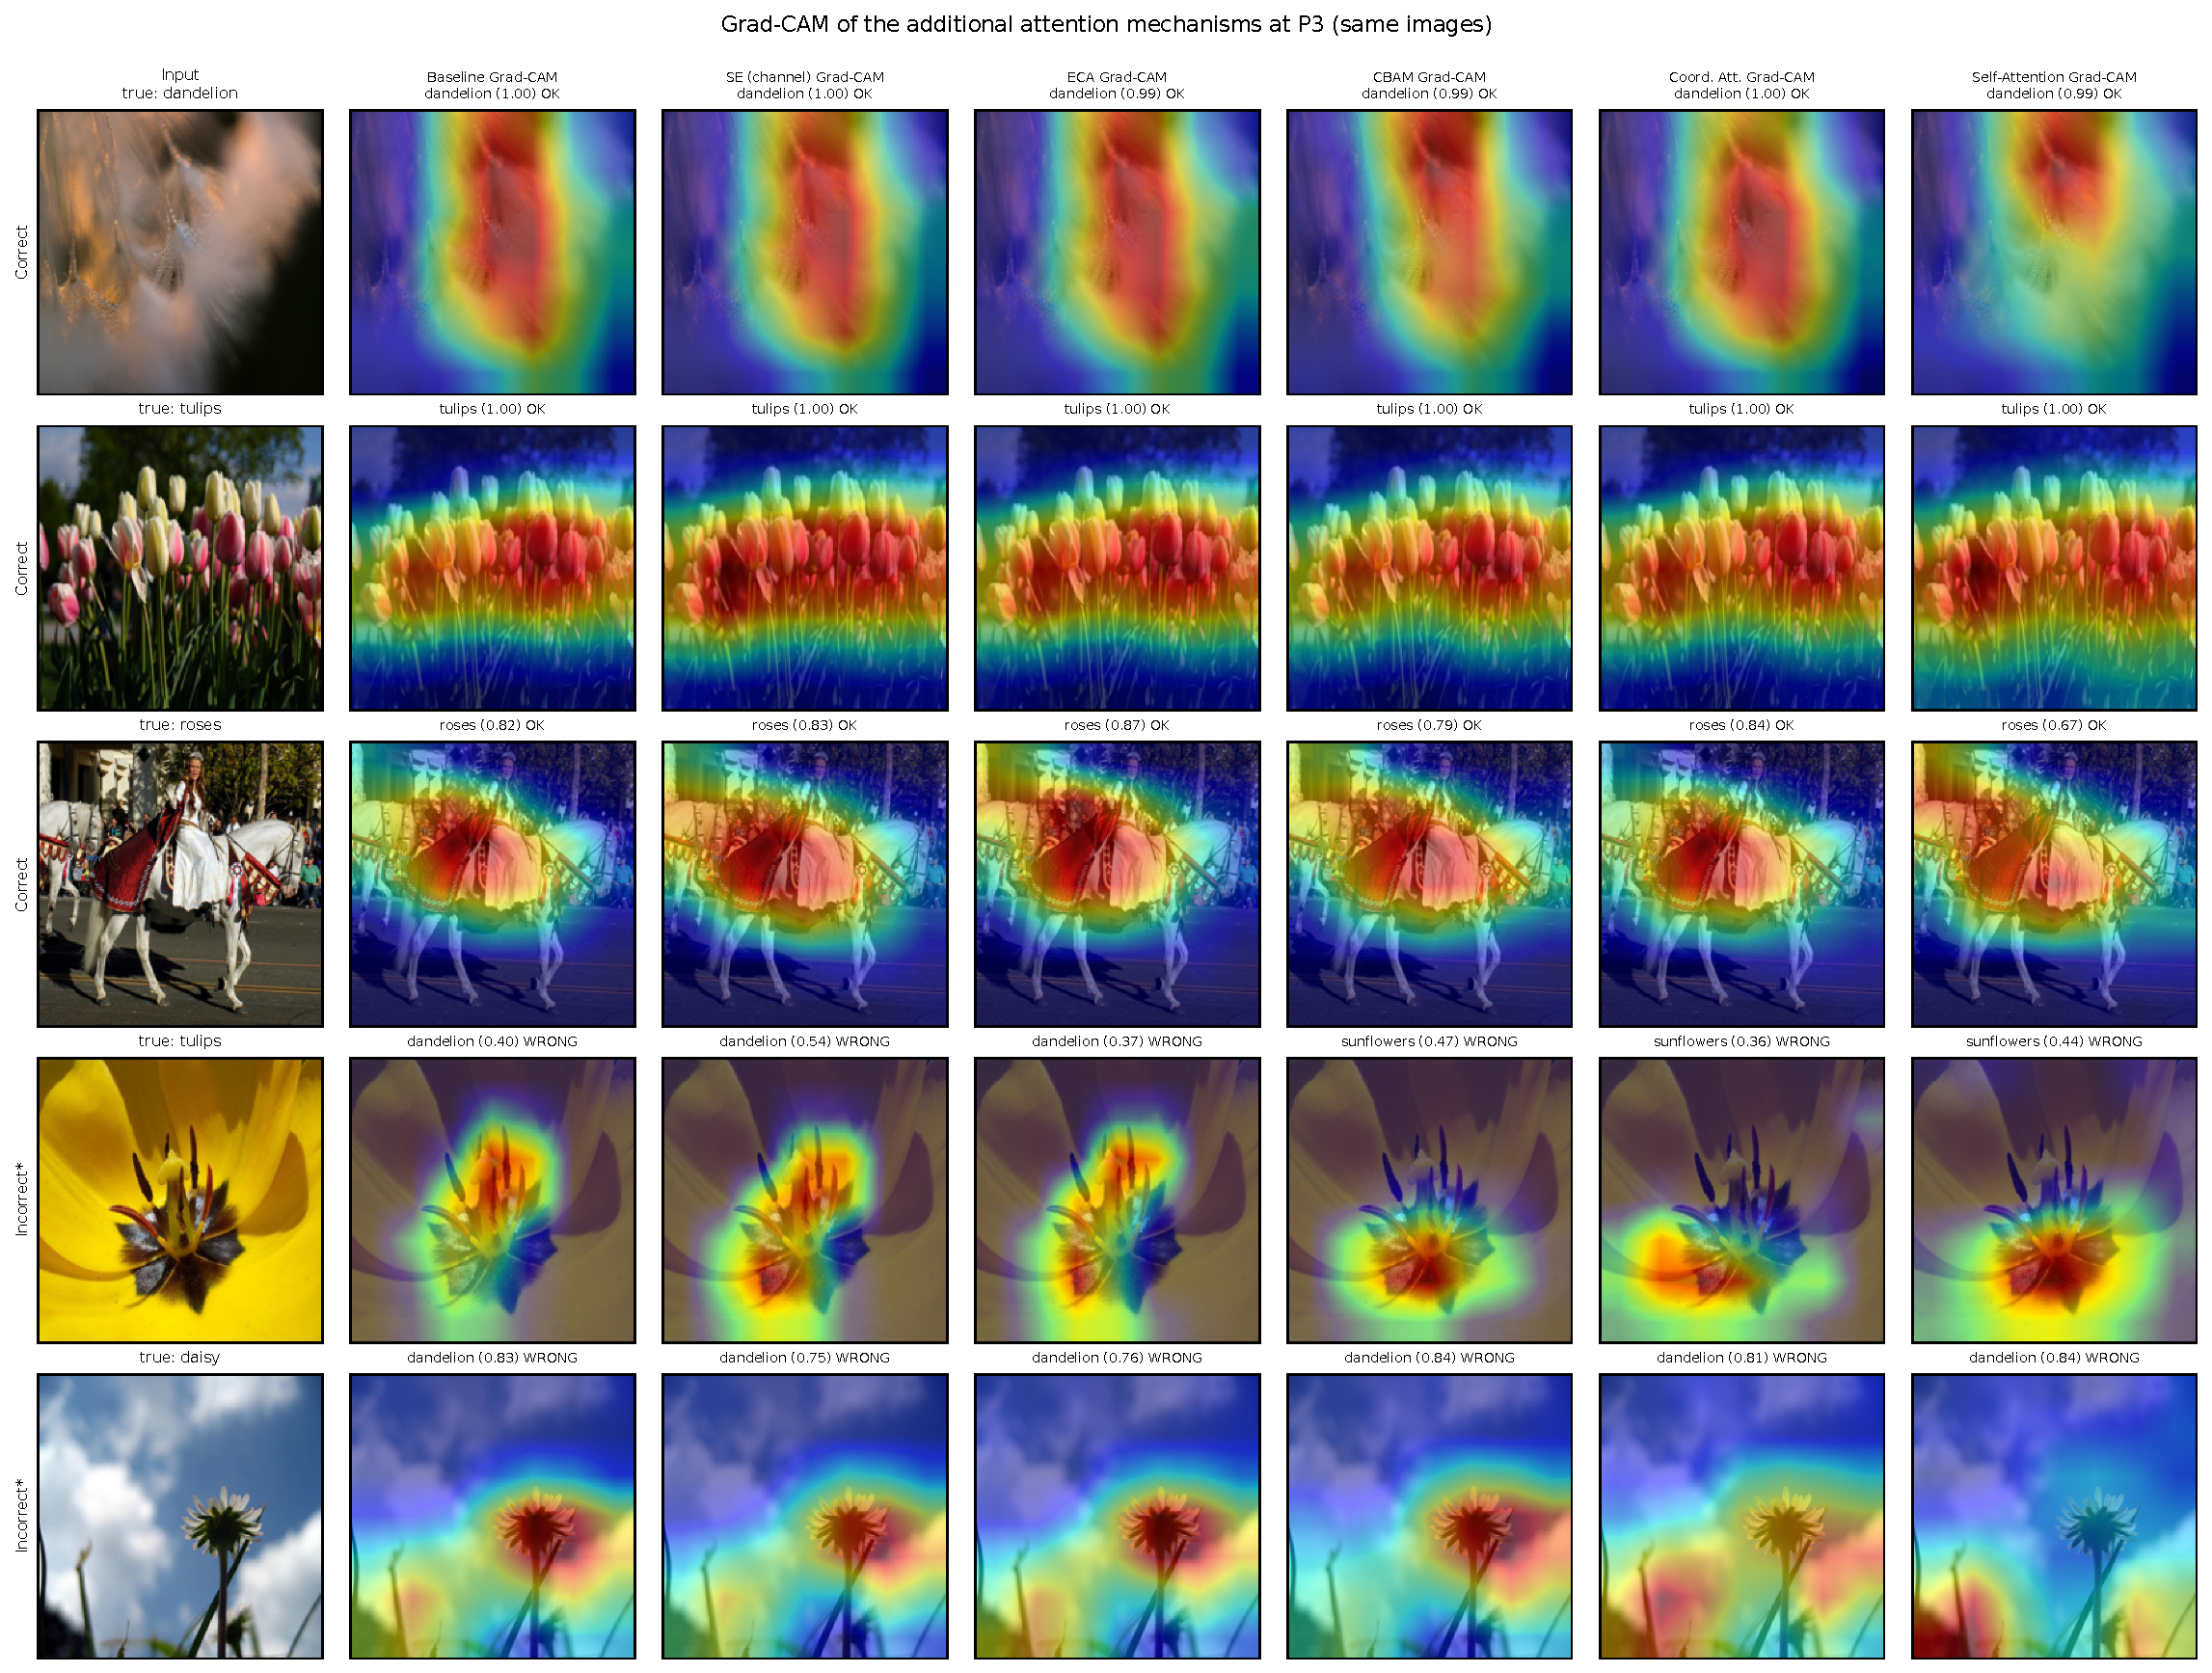
\includegraphics[width=\textwidth]{Images/use/F19_gradcam_additional_mechanisms.pdf}
\caption{Grad-CAM post-hoc visual explanations comparing Baseline against SE, ECA, CBAM, Coordinate Attention, and Self-Attention at stage $P_3$ across identical test images.}
\label{fig:f19_additional}
\end{figure}

\textbf{Inference:}All complex attention-enhanced architectures yield much more compact and foreground-oriented Grad-CAM maps than ResNet50 baseline without any augmentations. CBAM and Coordinate Attention exhibit the most prominent boundary containment by combining channel-wise attention selection with direction-sensitive spatial attention. Lightweight attention architectures such as ECA are as good at localizing features as heavy parameterized models, demonstrating that channel convolution with only one dimension of feature map yields enough discriminatory attention.

\vspace{3mm}

% ------------------------------------------------------------
\subsection*{30.19 Direct Grad-CAM Comparison: Baseline ResNet50 vs. Channel$\rightarrow$Spatial Attention}
% ------------------------------------------------------------

\begin{figure}[H]
\centering
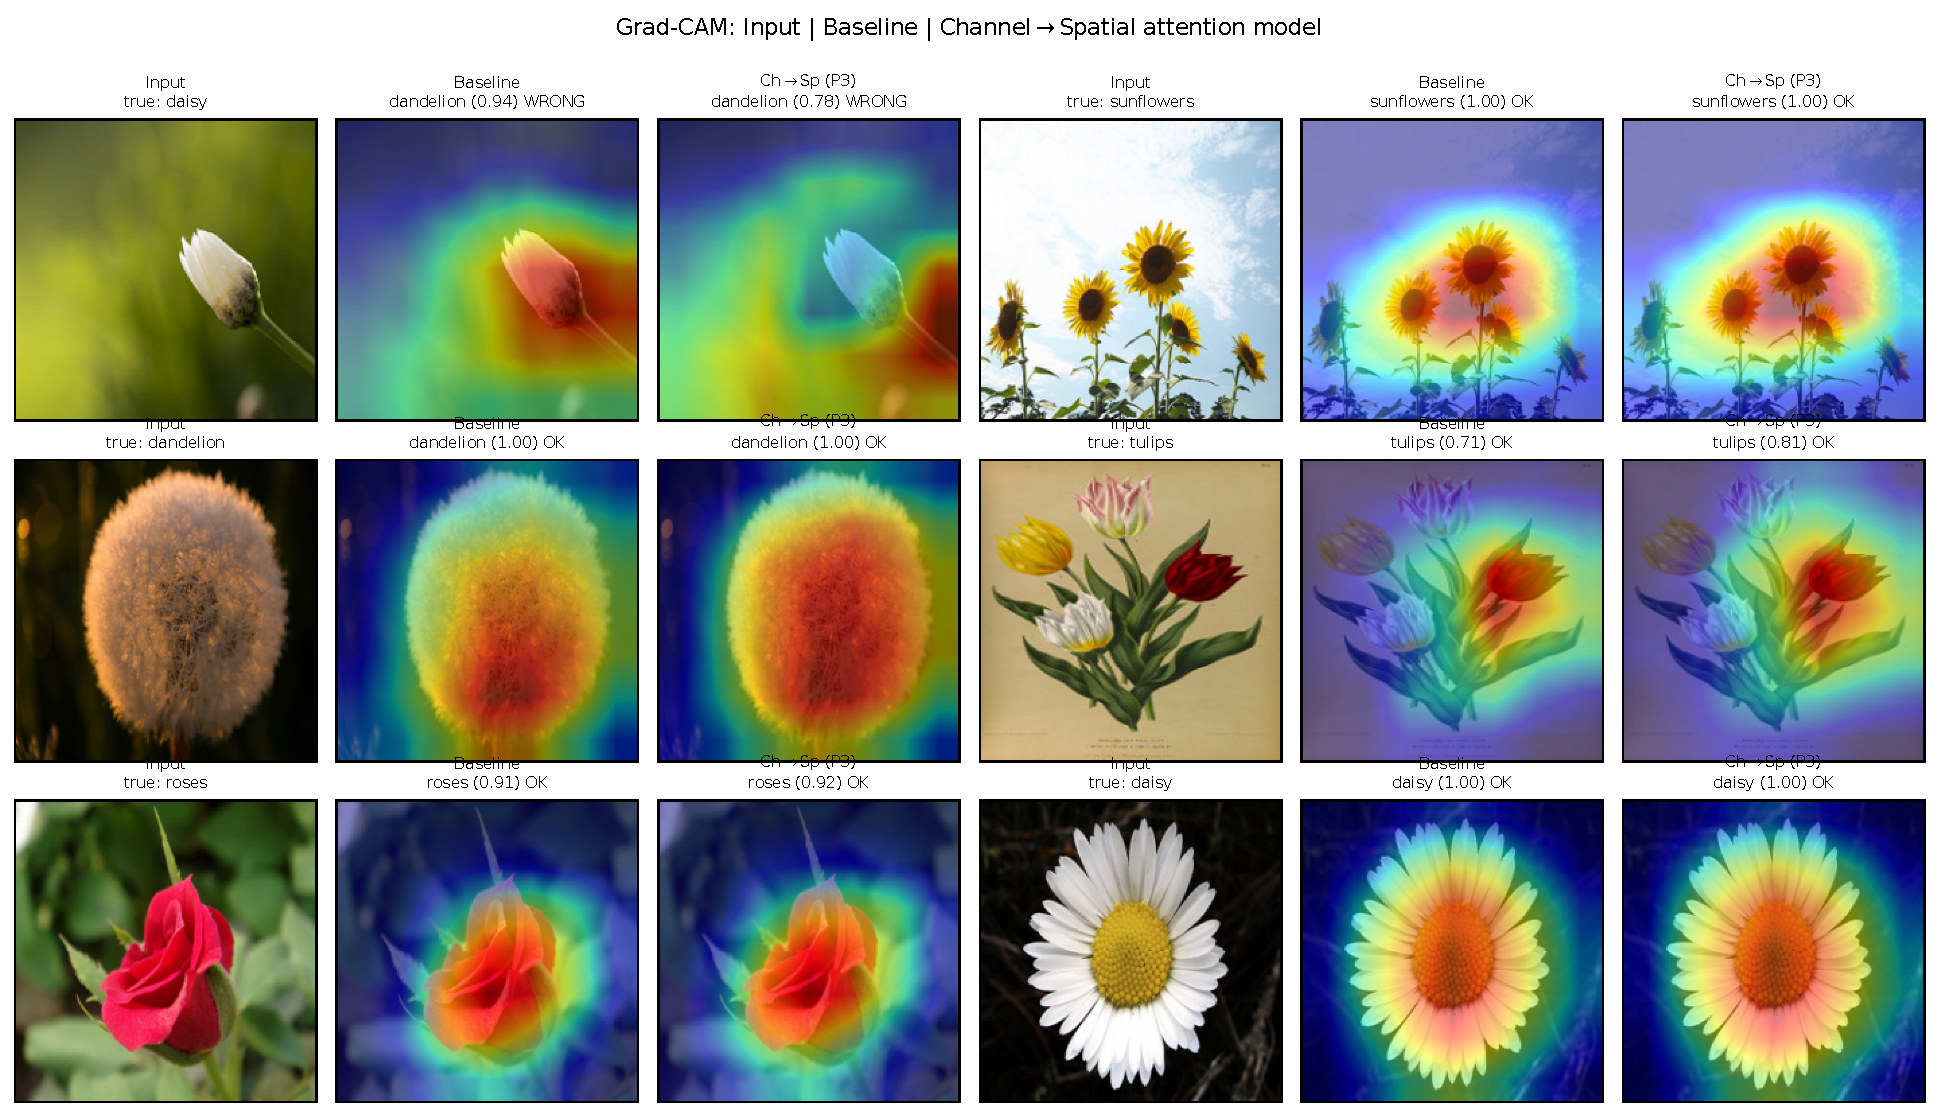
\includegraphics[width=\textwidth]{Images/use/F20_gradcam_baseline_vs_selected.pdf}
\caption{Direct pairwise Grad-CAM comparison between Baseline ResNet50 and Channel$\rightarrow$Spatial Attention ($P_3$) across multiple test instances of daisy, dandelion, roses, sunflowers, and tulips.}
\label{fig:f20_gradcam}
\end{figure}

\textbf{Inference:} The pairwise comparison shows that the Channel$\rightarrow$Spatial approach always removes the activations related to extraneous backgrounds in soil, lawn, and sky areas and leaves only those pertaining to the flowers' centers and petals. In the case of challenging examples, the attention-based approach improves the model's confidence scores for the prediction (for example, the confidence score for predicting tulips rises from 0.71 to 0.81), demonstrating a more certain model representation internally.

\vspace{3mm}

%%%%%%%%%%%%%%%%%%%%%%%%%%%%%%%%%%%%%%%%%%%%%%%%%%%%%%%%%%%%
\section*{31. Source Code }

\noindent\textbf{Source:} Github\\
\noindent\textbf{Github Repository Link:}

\url{https://github.com/ssvibitha/DeepLearningLab_2026-27/blob/main/Lab8_Attention/DL_Lab8.ipynb}

%%%%%%%%%%%%%%%%%%%%%%%%%%%%%%%%%%%%%%%%%%%%%%%%%%%%%%%%%%%%

% ============================================================
\section*{32. Discussion}
% ============================================================

\begin{enumerate}

\item \textbf{What is the purpose of residual connections in ResNet50?}

\textbf{Answer:} Residual connections offer shortcuts, which help the original feature information go through one or several layers without any interference. This way, training signals can easily propagate through the layers without being decreased, avoiding the vanishing gradient problem. The inclusion of residual connections guarantees that adding new layers will not decrease model performance and makes deep architectures easy to train.

\vspace{5mm}

\item \textbf{What does conv2\_x represent compared with conv5\_x?}

\textbf{Answer:} Conv2\_x is the stage of early vision features with detailed spatial dimensions and few channels. It detects edges, colors, and textures. On the other hand, conv5\_x is the stage of late semantic features with low-resolution spatial dimensions and many channels, which detect full object parts and classes. To summarize, conv2\_x shows the network where the fine-grained information is, while conv5\_x shows it what object is depicted.

\vspace{5mm}

\item \textbf{Why does the spatial resolution decrease with network depth?}

\textbf{Answer:} The spatial dimensions decrease due to pooling layers and strided convolutions, which make down-sampling of feature maps from one stage to another possible. It increases the receptive field of neurons, meaning that they can see bigger areas of an image as a whole.

\vspace{5mm}

\item \textbf{Why does the number of feature channels increase with network depth?}

\textbf{Answer:} More channels are used to compensate for the lack of spatial resolution through encoding rich and varied visual information. The deeper the layers, the greater the number of channels required to encode complex combinations of shapes, patterns, and objects identities. Through increasing the channel size, the network learns rich semantic representations required to discriminate between different flower classes.

\vspace{5mm}

\item \textbf{What is meant by low-level, intermediate, and high-level features?}

\textbf{Answer:} Low-level features are primitive visual features like edges, corners, colors, textures, etc., detected in early layers of the network. Intermediate features correspond to combinations of low-level features, which allow recognizing components of the objects, e.g., petal texture or flower center. Finally, high-level features correspond to abstract representations of the whole object in deep layers of the model.

\vspace{5mm}

\item \textbf{What is the purpose of an attention mechanism?}

\textbf{Answer:} The idea behind using attention is to allow the neural network to concentrate on informative features while ignoring useless noisy ones. Attention mechanism sets higher importance weight for specific spatial locations or feature channels during the forward pass of the network.

\vspace{5mm}

\item \textbf{What does channel attention attempt to learn?}

\textbf{Answer:} Channel attention is the technique of trying to understand which channel feature carries most of the information required to determine the correct class. The technique summarizes the entire channel for all spatial locations and then captures the interrelationships between channels. Through the weighting of the informative channels, it magnifies informative visual cues and minimizes uninformative ones.

\vspace{5mm}

\item \textbf{What does spatial attention attempt to learn?}

\textbf{Answer:} Spatial attention tries to understand the important spatial locations on an image or feature map for classification. It studies the interrelationship at all spatial locations to generate a two-dimensional importance map, which highlights the meaningful foreground objects, such as the petals and core of the flower, ignoring background regions, including leaves or soil.

\vspace{5mm}

\item \textbf{How is channel attention different from spatial attention?}

\textbf{Answer:} Channel attention determines what is important through assigning weights to different channels but treats all spatial locations the same way. On the other hand, spatial attention determines the important locations through weighting of the spatial locations but treats all channels the same way. To put it simply, channel attention chooses the best feature detectors, whereas spatial attention chooses the best image locations.

\vspace{5mm}

\item \textbf{Why can channel and spatial attention be used sequentially?}

\textbf{Answer:} They can be applied sequentially, since what they address are two complementary aspects of feature refinement along different dimensions. First, by applying channel attention, we highlight the most semantically relevant feature types, and second, by applying spatial attention, we pinpoint the region within which these features are present. By combining them step-by-step, a joint representation which incorporates both is formed.

\vspace{5mm}

\item \textbf{Why might channel attention behave differently at conv3\_x and
conv5\_x?}

\textbf{Answer:} As channels at \texttt{conv3\_x} encode intermediate pattern types, such as petal-shaped patterns, applying channel attention at this layer focuses on the most relevant types of mid-level texture detectors. On the other hand, since channels at \texttt{conv5\_x} encode abstract class specific concepts, attention over channels acts more like a selector of high-level category specific detectors. Hence, while channel attention in middle layers refines part detectors, it directly sharpens cues to the actual semantic class in deeper layers.

\vspace{5mm}

\item \textbf{Why can spatial attention be useful at an intermediate ResNet stage?}

\textbf{Answer:} An intermediate feature map still contains sufficient spatial resolution to encode relevant semantic information about the object parts. Hence, introducing spatial attention is a good opportunity to filter out the irrelevant contextual information before deeper semantic processing starts. This way, later layers can commit their representational capacity to the actual object of interest.

\vspace{5mm}

\item \textbf{Why is self-attention computationally expensive when the feature map
has high spatial resolution?}

\textbf{Answer:} Spatial self-attention calculates the interaction scores for each pair of any spatial location with any other spatial location from the feature map. When the spatial resolution becomes high, then the number of locations becomes extremely large, resulting in the increase in the computational cost for all the pairwise interactions being performed.

\vspace{5mm}

\item \textbf{What happens to the size of the self-attention matrix when the spatial
resolution increases?}

\textbf{Answer:} The size of the attention matrix increases exponentially with an increase in the total number of spatial locations. Doubling the spatial resolution will lead to a four-fold increase in the total number of locations and thus the attention matrix will be 16 times larger than before. This increase happens rapidly and the memory soon gets exhausted.

\vspace{5mm}

\item \textbf{How does attention performance vary when the insertion position is
changed?}

\textbf{Answer:} Attention inserted at an early stage does not provide much benefit since low-level features do not have semantic meanings while high resolution leads to high computation cost. Attention inserted at a later stage provides good trade-offs between semantic information and spatial information. Attention inserted at the late stage improves the concepts, but not the details that were lost at an early stage.

\vspace{5mm}

\item \textbf{How does attention at $P_2$ differ visually from attention at $P_4$?}

\textbf{Answer:} The visual attention maps at position two demonstrate high-resolution responses, highlighting the image’s edges, textures, and fine lines. In contrast, the attention maps at position four visualize low-resolution regions, covering entire semantic objects in the flower. The model at position two focuses on an image’s fine details, while the one at position four visualizes entire objects.

\vspace{5mm}

\item \textbf{Does applying attention at multiple stages always improve
classification performance?}

\textbf{Answer:} No, the attention module added at multiple stages does not necessarily improve the classification results. While the multiple attention blocks refine features repeatedly, they add extra parameters and can overfit on the few training samples. In most cases, adding a single attention block at a particular position improves the results with fewer parameters.

\vspace{5mm}

\item \textbf{Does Channel$\rightarrow$Spatial attention behave differently from
Spatial$\rightarrow$Channel attention?}

\textbf{Answer:} Yes, I think, implementing channel attention first improves the overall performance. This is because the channel attention determines which features are important, and, therefore, the spatial attention knows where to pay attention. On the other hand, if the spatial attention is implemented first, it will have to determine which channels to emphasize blindly.

\vspace{5mm}

\item \textbf{How does the spatial-attention kernel size influence the attention map?}

\textbf{Answer:} Using a bigger kernel, like seven by seven, can improve results because it covers a broader region, picking up global information and creating a soft attention mask. On the other hand, a three by three kernel covers only a small part of the image, and, therefore, the attention mask would be fragmented. As a result, a bigger kernel size is expected to visualize more relevant information in the image, thus producing better results.

\vspace{5mm}

\item \textbf{How does SE attention differ from ECA attention?}

\textbf{Answer:} The Squeeze-and-Excitation attention compresses channel dimensions using two dense layers and then restores them, thus leading to the addition of extra parameters and possible loss of some information. In contrast, Efficient Channel Attention does not involve any dimensionality reduction and uses one-dimensional convolution to capture the interaction of channels locally. Thus, ECA is much more efficient and accurate than the Squeeze-and-Excitation attention.

\vspace{5mm}

\item \textbf{How does CBAM combine channel and spatial attention?}

\textbf{Answer:} The CBAM attention network applies both channel and spatial attention through the usage of sequential connection of both attentions. It first performs channel attention through average and max pooling in order to re-weight feature channels. Afterward, it passes channel attention results to spatial attention, which emphasizes the most important spatial coordinates.

\vspace{5mm}

\item \textbf{How does self-attention differ from channel attention?}

\textbf{Answer:} In self-attention, all pairs of spatial positions are calculated in order to establish the relationships between the distant image pixels. Thus, the self-attention mechanism makes distant areas of an image able to communicate with each other. Channel attention establishes the relations between channels but does not take into account the relation between spatial points.

\vspace{5mm}

\item \textbf{Does the attention mechanism with the largest number of parameters
necessarily provide the highest accuracy?}

\textbf{Answer:} No, the largest number of parameters does not necessarily deliver the highest accuracy. Heavier attention modules may easily overfit medium-sized datasets, and introduce instabilities in training. In practice, lighter attention designs often match or exceed the accuracy, by generalizing better, while incurring only a negligible overhead.

\vspace{5mm}

\item \textbf{What is the difference between an internal attention map and Grad-CAM?}

\textbf{Answer:} An internal attention map is an explicit set of weights calculated inside the network layers during the forward pass, while Grad-CAM is an explanation heatmap generated post-hoc, by flowing the gradients backwards from the output class score through the network.

\vspace{5mm}

\item \textbf{Why is Grad-CAM called a post-hoc explanation technique?}

\textbf{Answer:} Grad-CAM is called post-hoc because it is computed after the model has already completed its forward prediction. It does not change the internal processing of the model’s features, but rather analyzes the existing weights by performing gradient descent in the reverse direction. Thus, Grad-CAM can be considered as an external diagnostic tool that evaluates the model decisions after they have been made.

\vspace{5mm}

\item \textbf{Does the attention model suppress irrelevant background regions?}

\textbf{Answer:} Yes, the attention model is effective in suppressing the irrelevant background regions such as grass, dirt, and leaves, by reducing their weights. Similarly, it removes the background spatial locations, preventing their features from being used downstream in the classification process.

\vspace{5mm}

\item \textbf{Are the attention maps of correctly classified and incorrectly
classified images different?}

\textbf{Answer:} Yes, properly classified images have attention maps that are sharp and concentrated in the region right on the center of the flower petals. Misclassified images, on the other hand, will generally exhibit dispersed or scattered attention maps and sometimes misfocus on the leaves and other elements in the image. This is proof that misclassification is due to the network being misled by its attention.

\vspace{5mm}

\item \textbf{Which flower classes benefit most from attention?}

\textbf{Answer:}  Classes with natural cluttered backgrounds and having high similarity with other classes will benefit the most from attention. Examples are classes like flowers such as daisy and dandelion whose accuracy benefits the most from attention since this mechanism distinguishes fine petals from cluttered grassy backgrounds. Classes with simple backgrounds and unique colors benefit much less.

\vspace{5mm}

\item \textbf{What information can be obtained from a confusion matrix that cannot
be obtained from overall accuracy alone?}

\textbf{Answer:} A confusion matrix will show exactly which classes of flower the model often confuses with one another. It will be evident which class pairs are hard for the model to distinguish. Accuracy gives a summary score of overall performance while ignoring which particular classes are having misclassification problems.

\vspace{5mm}

\item \textbf{Why is macro F1 useful in addition to accuracy?}

\textbf{Answer:} Macro F1 evaluates the unweighted average of the performance of all the classes. This way, each class is equally important, and the high performance of the model on the frequent classes does not “hide” its low performance on the rare classes. It should give a more honest estimation of how well the model classifies different types of flowers.

\vspace{5mm}

\item \textbf{What is meant by the accuracy--complexity trade-off?}

\textbf{Answer:} The accuracy–-complexity trade-off refers to how much model performance improves (i.e., accuracy increases) with adding complexity (more parameters) to the model. In other words, it is a ratio of how much accuracy increases and complexity grows when one adjusts the hyperparameters during training. A good model should have the best accuracy–complexity ratio, theoretically providing the best possible accuracy with the minimal required complexity.

\vspace{5mm}

\item \textbf{What is meant by the F1--inference-time trade-off?}

\textbf{Answer:} The F1–inference-time trade-off is similar to the accuracy–complexity trade-off but concerns the amount of time needed to make predictions with the model. Essentially, it is a ratio of how much F1 increases and inference time grows with added complexity. A good model should have the best F1–inference-time trade-off, theoretically providing the best possible F1 with the lowest possible inference time.

\vspace{5mm}

\item \textbf{Why must every ablation study use the same dataset split?}

\textbf{Answer:} Using the same dataset split allows for consistent results. Otherwise, if one randomly generates splits for the dataset, there is a possibility of getting a relatively “easy” split, resulting in higher than average accuracy and performance. By using the same split, one gets the unbiased estimate of the model’s performance.

\vspace{5mm}

\item \textbf{Why must the same training protocol be maintained when comparing
different attention mechanisms?}

\textbf{Answer:} Training identical parameters such as learning rate, optimization function, batch size, and epochs helps us get the true impact of each attention module because otherwise we will not be able to distinguish the effects of either changing training parameters or changing the model architecture. In addition, this approach is necessary for us to test our models on a truly equal footing.

\vspace{5mm}

\item \textbf{What conclusions can be drawn from the Grad-CAM comparison?}

\textbf{Answer:} Comparing Grad-CAM maps allows us to confirm visually the fact that attention modules indeed make heatmaps tighter, allowing us to see discriminative parts of flowers better than the baseline model does. In addition, this fact proves visually that the attention module helps suppress background noise.

\vspace{5mm}

\end{enumerate}


% ============================================================
\section*{33. Expected Outcome}
% ============================================================

At the end of the experiment, students should understand that an attention
mechanism is not an isolated module whose behavior is independent of the
backbone.

Its effectiveness depends on:

\[
\boxed{
\begin{aligned}
\text{Attention Effectiveness}
={}&
\text{Attention Type}\\
&+
\text{Attention Position}\\
&+
\text{Feature Resolution}\\
&+
\text{Feature Semantics}\\
&+
\text{Model Complexity}.
\end{aligned}
}
\]

Students should also understand that classification performance alone does
not provide a complete explanation of an attention mechanism.

A comprehensive analysis should therefore combine:

\[
\boxed{
\text{Classification Performance}
}
\]

with

\[
\boxed{
\text{Computational Complexity}
}
\]

and

\[
\boxed{
\text{Qualitative Visualization}.
}
\]

Therefore:

\[
\boxed{
\text{Complete Attention Analysis}
=
\text{Quantitative}
+
\text{Computational}
+
\text{Qualitative}
}
\]

The final conclusions must be based on the student's experimental results
rather than on assumptions about which attention mechanism should perform
best.

% ============================================================
\section*{34. References}
% ============================================================

\begin{enumerate}

\item
K. He, X. Zhang, S. Ren, and J. Sun,
``Deep Residual Learning for Image Recognition,''
\textit{Proceedings of the IEEE Conference on Computer Vision and Pattern
Recognition (CVPR)}, pp. 770--778, 2016.

\item
J. Hu, L. Shen, S. Albanie, G. Sun, and E. Wu,
``Squeeze-and-Excitation Networks,''
\textit{IEEE Transactions on Pattern Analysis and Machine Intelligence},
vol. 42, no. 8, pp. 2011--2023, 2020.

\item
S. Woo, J. Park, J.-Y. Lee, and I. S. Kweon,
``CBAM: Convolutional Block Attention Module,''
\textit{Proceedings of the European Conference on Computer Vision (ECCV)},
pp. 3--19, 2018.

\item
Q. Wang, B. Wu, P. Zhu, P. Li, W. Zuo, and Q. Hu,
``ECA-Net: Efficient Channel Attention for Deep Convolutional Neural
Networks,''
\textit{Proceedings of the IEEE/CVF Conference on Computer Vision and Pattern
Recognition (CVPR)}, pp. 11534--11542, 2020.

\item
Q. Hou, D. Zhou, and J. Feng,
``Coordinate Attention for Efficient Mobile Network Design,''
\textit{Proceedings of the IEEE/CVF Conference on Computer Vision and Pattern
Recognition (CVPR)}, pp. 13713--13722, 2021.

\item
A. Vaswani et al.,
``Attention Is All You Need,''
\textit{Advances in Neural Information Processing Systems},
vol. 30, 2017.

\item
R. R. Selvaraju, M. Cogswell, A. Das, R. Vedantam,
D. Parikh, and D. Batra,
``Grad-CAM: Visual Explanations from Deep Networks via
Gradient-Based Localization,''
\textit{Proceedings of the IEEE International Conference on Computer Vision
(ICCV)}, pp. 618--626, 2017.

\item
TensorFlow Documentation:
\url{https://www.tensorflow.org/}

\item
Keras Documentation:
\url{https://keras.io/}

\item
TensorFlow Datasets:
\url{https://www.tensorflow.org/datasets}

\end{enumerate}

% ============================================================
% END DOCUMENT
% ============================================================

\end{document}
